%\chapter{\Objectivetwoname}
\chapter[Takens-based Kernel \gls{te} Connectivity Network for \gls{mi} Classification]{Takens-based Kernel \gls{te} Connectivity Network for
\gls{mi} Classification}\label{chapter_2} 
\chaptermark{TEKTE-Net}


\noindent\noindent{\textbf{Interpretative note on causal terminology.}
This chapter is based on a peer-reviewed article previously published by the author 
and included here as part of a unified doctoral research framework. Therefore, the 
methodological terminology of the original publication is preserved. However, in light 
of the discussion presented in Section~\ref{sec:causality_eeg}, the terms 
\emph{causal}, \emph{causal influence}, \emph{causal dependencies}, 
\emph{inter-channel causality}, and related expressions used in this chapter should 
be interpreted in the predictive Wiener--Granger sense commonly adopted in 
neuroscience. Accordingly, \gls{te}-based connectivity is understood here as directed 
information flow or directed predictive dependency at the signal level, rather than as 
definitive evidence of strict interventional, counterfactual, or mechanistic causality.}

%introduccion de 2 parrafos 
Building upon the foundations established by the Gaussian Connectivity-Driven \gls{eeg} Imaging framework, which focused on enhancing functional representation and spatial interpretability, the next step in this research addresses the modeling of effective brain connectivity. While functional connectivity captures statistical dependencies between neural regions, it does not account for the directionality or causal influence of information flow within the brain. Such directional and dynamic interactions are critical for understanding the neural mechanisms underlying motor control and cognitive processing, particularly in \gls{mi} paradigms. Consequently, there is a growing need for computational models that can infer nonlinear and time-dependent relationships directly from \gls{eeg} data, while maintaining interpretability and robustness.

To meet this challenge, {this contribution} introduces the Takens-Based Enhanced Kernel \gls{te}  Network (\gls{tektenet}), a novel deep learning framework designed to estimate and learn directed and nonlinear interactions in \gls{eeg} signals. \gls{tektenet} combines Takens' state-space reconstruction with kernel-based \gls{te}  estimation, allowing the network to represent causal dependencies within a latent connectivity space. By embedding this information into a deep generative model, the framework captures both the temporal dynamics and directional flow of neural activity, bridging the gap between effective connectivity analysis and end-to-end \gls{eeg} decoding. This contribution represents a crucial step toward the development of adaptive, interpretable, and causally informed \gls{bci} systems.

{It is important to clarify that \gls{tektenet} is not intended to replace classical event-related potential (ERP) analysis, nor should it be interpreted as a deeper version of ERP-based evaluation. ERP analysis mainly characterizes time-locked cortical responses in terms of amplitude, latency, and waveform morphology~\cite{Picton2000ERP}. In contrast, \gls{tektenet} aims to provide complementary network-level information by estimating nonlinear, directed, and time-delayed interactions between \gls{eeg} channels. Therefore, while ERP analysis can indicate when a cognitive or sensorimotor response occurs, \gls{tektenet} seeks to characterize how information flows across reconstructed \gls{eeg} state spaces during task-related brain dynamics.}


Figure~\ref{fig:tekte_pipeline} provides a schematic overview of the proposed framework, illustrating the main processing stages from raw \gls{eeg} signals to the estimation of directed connectivity patterns for \gls{mi} classification.

\begin{figure}[htbp]
  \centering
  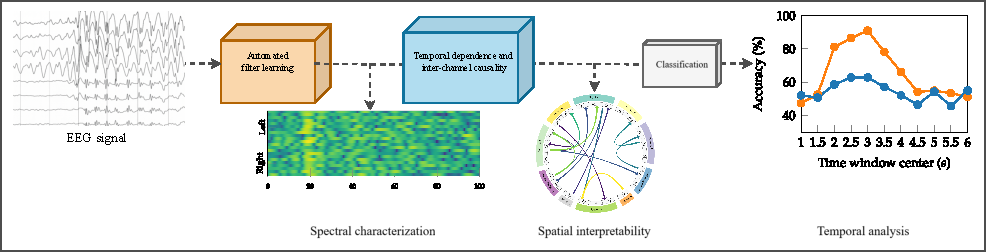
\includegraphics[width=\textwidth]{Figures/Metodology.pdf}
  \caption{Schematic overview of the proposed connectivity-driven framework for \gls{mi} classification. 
  Raw \gls{eeg} signals are processed through automated filter learning and temporal modeling to capture nonlinear and directed inter-channel interactions. 
  The resulting representations enable spectral characterization, spatial interpretability through connectivity patterns, and temporal analysis of task-related dynamics.}
  \label{fig:tekte_pipeline}
\end{figure}

\subsection{Mathematical Framework}\label{sec:Mathematical_Framework}

{This contribution} introduces \gls{tektenet}, a novel end-to-end deep learning architecture designed to model nonlinear spatiotemporal dynamics and directed causal interactions directly from raw \gls{eeg}signals. The model incorporates a customized convolutional module that performs Takens' embedding, enabling the reconstruction of the underlying dynamical system without requiring explicit preprocessing. This mechanism facilitates the extraction of subject-specific, task-relevant temporal and spectral features. A central contribution of \gls{tektenet} is the integration of a fully differentiable \gls{te} estimator, formulated via Rényi's $\alpha$-order entropy and positive-definite kernels, allowing for the estimation of nonlinear, directed information flow between \gls{eeg}channels within a trainable framework. The following sections describe the dataset and mathematical foundations in detail.

\subsubsection{Channel-wise nonlinear time series embedding from Takens' convolutional layer}\label{sec:takens}

Let $\mat{X} \in \mathbb{R}^{T \times C}$ be a discrete multichannel input signal of temporal length $T$ and $C$ channels. The channel-wise nonlinear filtering of the $c$-th channel is denoted as $\ve{\phi}_c=\varphi(\ve{x}_c|\theta_c)$, being $\ve{x}_c\in\Real^T$ its corresponding input time series, $\ve{\phi}_c\in\Real^{T_{\phi}}$ the filtered output of length $T_{\phi}\leq T$. A deep learning strategy nonlinearly filters each channel using $L$ sequential layers parameterized by $\theta_c$, that is, $\varphi(\cdot|\theta_c)=\varphi_{L}(\cdots(\varphi_1(\cdot))$. The usual layers considered in the nonlinear filtering are convolutions, poolings, and dropouts that support extracting complex channel-wise temporal structures and nonlinear dependencies to learn more informative and discriminative representations.

Aiming to take advantage of the \gls{eeg}latent dynamics through the Markovian property, a delay-coordinate Takens' embedding reconstructs the channel-wise state space by stacking time-delayed versions of the nonlinearly-filtered channel $\ve{\phi}_c$ into fixed-length vectors, resulting in a delay-embedded representation $\mat{Z}_{c\mu} \in \mathbb{R}^{T_z \times D}$, where $D \in \mathbb{N}$ denotes the embedding order (i.e., number of delay coordinates), the delay offset $\mu \in \mathbb{N}$, and $T_z\leq T_\phi$. A set of fixed, non-trainable convolutional filters implements the embedding replicating delayed copies of the input without altering the learned parameters as 
\begin{equation}\label{eq:z_takens}
\mat{Z}_{c\mu}=\mat{W}_{D,\tau,\mu}^\top*\ve{\phi}_c
\end{equation}
{where the convolution kernel $\mat{W}_{D,\tau,\mu}\in\{0,1\}^{R \times D}$, with $R = \mu + \tau \cdot (D - 1) + 1$,} depends on three predefined hyperparameters, namely, the delay stride $\tau \in \mathbb{N}$, the embedding order $D$, and the delay offset $\mu$. Such Takens' convolution kernel elements holds elements 
$w_{r,d}=\delta(r - \mu - \tau \cdot d)\forall d \in [0, D-1], r \in [0, {R}-1]$, with $\delta(\cdot)$ as the discrete delta Dirac function. Thus, the full Takens-embedded nonlinearly-filtered signal $\mat{Z}_{c\mu}$ enables the subsequent processing layers to access the temporal structure and to capture directed inter-channel interactions through the reconstructed dynamical states rather than raw observations.

\subsubsection{\gls{te}  from kernel matrices}

{This contribution} assesses the inter-channel interactions through the \gls{te}  which has been proposed as an effective tool for distinguishing between driving and responding elements, as well as for detecting asymmetries in subsystem interactions~\cite{staniek2008symbolic}. Originally introduced by Schreiber~\cite{schreiber2000measuring} and related to the concept of Granger causality~\cite{Sethgranger}, TE operates under the premise that the $c$-th channel $\ve{x}_{c}$ can be considered to causally influence $c'$-th channel $\ve{x}_{c'}$ if incorporating the past of the channel $c$, together with the past of channel $c'$, better predicts the present of $\ve{x}_{c'}$ than using $\ve{x}_{c'}$ past alone, for all discrete time instants $t\in[1,T]$. According to \Cref{sec:takens}, the present of the responding channel $c'$ can be computed from the Takens' delayed-embedding by setting $\mu=0$ and $D=1$, while its past by setting $\mu=1$ and $D=D'$ to be tuned, respectively. In turn, the past of the driving channel $c$ accounts for $D$ time-delayed interactions, thanks to $\mu$, as in \Cref{eq:xt-u}.
\begin{align}
\ve{z}_{c'0}=&\mat{W}_{\tau,1,0}^\top*\ve{\phi}_{c'}\in\Real^{T_z}\label{eq:yt}\\
\mat{Z}_{c'1}=&\mat{W}_{\tau,D',1}^\top*\ve{\phi}_{c'}\in\Real^{T_z\times D'}\label{eq:yt-1}\\
\mat{Z}_{c\mu}=&\mat{W}_{\tau,D,\mu}^\top*\ve{\phi}_c\in\Real^{T_z\times D}\label{eq:xt-u}
\end{align}

Note that the $t$-th row of the Takens' embeddings in \Cref{eq:yt,eq:yt-1,eq:xt-u} correspond to the current state of the responding channel $z_{c't}\in\Real$, the past state of the responding channel $\ve{z}_{c't-1}\in\Real^D$, and the past of the driving channel $\ve{z}_{ct-\mu}\in\Real^D$, respectively, aligned at every time instant $t\in[1,T_z]$. Using those three time-aligned embeddings, \Cref{eq:te_01} formally defines the \gls{te}  $TE(c \to c')$ as the expected information gain about the current state of the responding channel given its own past, i.e., $p\left(z_{c't} \mid \ve{z}_{c't-1}\right)$, when the past of the driving channel is also known, i.e.,  $p\left(z_{c't} \mid \ve{z}_{c't-1},\,\ve{z}_{ct-\mu}\right)$. 
\begin{equation}
    TE(c \to c') = 
    \iiint 
    p\bigl(z_{c't},\,\ve{z}_{c't-1},\,\ve{z}_{ct-\mu}\bigr)\, 
    \log\!\biggl(
      \frac{ 
        p\bigl({z}_{c'} \mid \ve{z}_{c't-1},\,\ve{z}_{ct-\mu}\bigr)
      }{
        p\bigl({z}_{c'} \mid \ve{z}_{c't-1}\bigr)
      }
    \biggr)
    \,d{z}_{c'}\,d\ve{z}_{c't-1}\,d\ve{z}_{ct-\mu}.
\label{eq:te_01}
\end{equation}
Equivalently, it can be written in expectation form as:
\begin{equation}
    TE(c \to c') \;=\; 
\mathbb{E}_{z_{c't},\,\ve{z}_{c't-1},\,\ve{z}_{ct-\mu}}
\Biggl\{
  \log\!\biggl(
    \frac{ 
      p\bigl(z_{c't} \mid \ve{z}_{c't-1},\,\ve{z}_{ct-\mu}\bigr)
    }{
      p\bigl(z_{c't} \mid \ve{z}_{c't-1}\bigr)
    }
  \biggr)
\Biggr\},
\end{equation}
where the expectation operator is defined as 
\begin{equation}
    \mathbb{E}_{z}\{f(z)\} \;=\; \int p(z)\,f(z)\,dz.
\end{equation}

Thanks to Bayes’ rule and logarithm properties, the conditional probabilities in Equation~\eqref{eq:te_01} are split into four terms depending on the joint and marginals as follows:
\begin{align}
 TE(c \to c') &= \mathbb{E}_{z_{c't},\ve{z}_{c't-1},\ve{z}_{ct-\mu}}
      \bigl\{\log p\bigl(z_{c't},\ve{z}_{c't-1},\ve{z}_{ct-\mu}\bigr)\bigr\} \label{eq:TE_expansion1}\\
      &-\mathbb{E}_{z_{c't},\ve{z}_{c't-1},\ve{z}_{ct-\mu}}
      \bigl\{\log p\bigl(\ve{z}_{c't-1},\ve{z}_{ct-\mu}\bigr)\bigr\}\nonumber\\
      &+\mathbb{E}_{z_{c't},\ve{z}_{c't-1},\ve{z}_{ct-\mu}}
      \bigl\{\log p\bigl(\ve{z}_{c't-1}\bigr)\bigr\}\nonumber\\
      &-\mathbb{E}_{z_{c't},\ve{z}_{c't-1},\ve{z}_{ct-\mu}}
      \bigl\{\log p\bigl(z_{c't},\ve{z}_{c't-1}\bigr)\bigr\}.\nonumber
\end{align}

Since the arguments of the logarithm are marginalizations of $p(z_{c't},\ve{z}_{c't-1},\ve{z}_{ct-\mu})$, the expectations are constant on the remaining variables and reduce to:
\begin{align}
 TE(c \to c') &= \mathbb{E}_{z_{c't},\ve{z}_{c't-1},\ve{z}_{ct-\mu}}
      \bigl\{\log p\bigl(z_{c't},\ve{z}_{c't-1},\ve{z}_{ct-\mu}\bigr)\bigr\} \label{eq:TE_02}\\
      &-\mathbb{E}_{\ve{z}_{c't-1},\ve{z}_{ct-\mu}}
      \bigl\{\log p\bigl(\ve{z}_{c't-1},\ve{z}_{ct-\mu}\bigr)\bigr\}\nonumber\\
      &+\mathbb{E}_{\ve{z}_{c't-1}}
      \bigl\{\log p\bigl(\ve{z}_{c't-1}\bigr)\bigr\}\nonumber\\
      &-\mathbb{E}_{z_{c't},\ve{z}_{c't-1}}
      \bigl\{\log p\bigl(z_{c't},\ve{z}_{c't-1}\bigr)\bigr\}.\nonumber
\end{align}

Noting that each term in \Cref{eq:TE_02} matches the Shannon entropy definition of $H_S(Z)=-\mathbb{E}_{z}\{\log p(z)\},$ the information gain of the \gls{te}  is finally rewritten in terms of joint and marginal entropies as in~\Cref{eq:TE_03}. For the sake of visual understanding, \Cref{fig:venn} illustrates the relationship between the random variables and its entropies in the estimation of the \gls{te} .
\begin{align}
  TE(c \to c') &= -H_S\bigl\{z_{c't},\ve{z}_{c't-1},\ve{z}_{ct-\mu}\bigr\}
  +H_S\bigl\{\ve{z}_{c't-1},\ve{z}_{ct-\mu}\bigr\}\label{eq:TE_03}\\
  &-H_S\bigl\{\ve{z}_{c't-1}\bigr\}+H_S\bigl\{z_{c't},\ve{z}_{c't-1}\bigr\}.\nonumber
\end{align}
%-----------------------------------------------------------------
\begin{figure}[htbp]
  \centering
  \subfloat[0.2\columnwidth][\centering\footnotesize$H_S\{z_{c't},\ve{z}_{c't-1},\ve{z}_{ct-\mu}\}$]{\input{Figures/venn_joint} \label{fig:venn_joint}}
  \subfloat[0.2\columnwidth][\centering\footnotesize$H_S\{\ve{z}_{c't-1},\ve{z}_{ct-\mu}\}$]{\input{Figures/venn_ccp} \label{fig:venn_ccp}}
  \subfloat[0.2\columnwidth][\centering\footnotesize$H_S\{\ve{z}_{c't-1}\}$]{\input{Figures/venn_cp} \label{fig:venn_cp}}
  \subfloat[0.2\columnwidth][\centering\footnotesize$H_S\{z_{c't},\ve{z}_{c't-1}\}$]{\input{Figures/venn_cpcp} \label{fig:venn_cpcp}}\\
  \subfloat[0.2\columnwidth][\centering\footnotesize$\mathrm{TE}(c \to c')$]{\centering\input{Figures/venn_TE} \label{fig:venn_TE}}
  \caption{Venn diagrams illustrating the definition of \gls{te}  from joint and marginal Shannon entropies. Circles correspond to the responding channel present $z_{c',t}$, the Takens-embedded responding's past $\ve{z}_{c',t-1}$, and the Takens-embedded driving's past $\ve{z}_{c,t-\mu}$. The \gls{te}  identifies the unique predictive information from the driving's past to the responding's present beyond the responding's own history.}
  \label{fig:venn}
\end{figure}
%-----------------------------------------------------------------

To calculate TE from discrete data, the Shannon entropies in \Cref{eq:TE_03} require the estimation of joint and marginal probability distributions, which are often intractable. For avoiding the explicit estimation of these distributions, {this contribution} adopts a kernel-based approximation of Shannon joint and marginal entropies from discrete observations over finite state spaces, as defined in \Cref{eq:SA,eq:SAB} respectively, being $\ve{v}$ and $\ve{v}'$ are two random vectors~\cite{giraldo2015measures}. The Gram matrices $\mat{K}_{\ve{v}}$ and $\mat{K}_{\mat{v}'}$ capture the covariance structure of the vector-valued random variables $\ve{v}$ and $\ve{v}'$ in a Reproducing Kernel Hilbert Space (RKHS), and $\circ$ denote the Hadamard product operator.

\begin{align}
    H\left\{\ve{v}\right\} &\approx S(\mat{K}_{\ve{v}}) = \log\left(\text{trace}\left(\mat{K}_{\ve{v}}\right)\right) \label{eq:SA}\\
    H\left\{\ve{v},\ve{v'}\right\} &\approx S\left(\frac{\mat{K}_{\ve{v}} \circ \mat{K}_{\ve{v}'}}{\text{trace}\left(\mat{K}_{\ve{v}} \circ \mat{K}_{\ve{v}'}\right)}\right)\label{eq:SAB} 
\end{align}
Above estimators approximate the \gls{te}  in \Cref{eq:TE_03} as:
\begin{align}
TE_{cc'} \approx& -S\left( \mat{K}_{c'{0}}, \mat{K}_{c'{1}}, \mat{K}_{c{\mu}} \right)
+ S\left( \mat{K}_{c'{1}}, \mat{K}_{c{\mu}} \right) \label{eq:TE_k}\\
&- S\left( \mat{K}_{c'{1}} \right) + S\left( \mat{K}_{c'{0}}, \mat{K}_{c'{1}} \right),\nonumber\\
\mat{K}_{c'0} =& \left[ \kappa({z}_{c't},{z}_{c's}\mid \ell_{c'0}) \right]_{t,s=1}^{T_z}\label{eq:ky}\\
\mat{K}_{c'1} =& \left[ \kappa(\ve{z}_{c't-1},\ve{z}_{c's-1}\mid \ell_{c'1}) \right]_{t,s=1}^{T_z}\label{eq:ky-1}\\
\mat{K}_{c\mu} =& \left[ \kappa(\ve{z}_{ct-\mu},\ve{z}_{cs-\mu}\mid \ell_{c\mu}) \right]_{t,s=1}^{T_z}\label{eq:kx}.
\end{align}
where the kernel matrices $\mathbf{K}_{c'0},\mathbf{K}_{c'{1}},\mathbf{K}_{c,{\mu}} \in \Real^{T_z \times T_z}$ hold the covariances of the responding channel present, its past, and the driving channel past, respectively. 

All the three kernel matrices are computed by a positively defined kernel function reproducing a Hilbert space $\kappa(\cdot, \cdot\mid\ell)$ which holds the parameter set $\ell$. Particularly, {this contribution computes} the similarities between time series using the Rational Quadratic (RQ) kernel as it generalizes the Gaussian by accommodating multi-scale variation. \Cref{eq:rqk} defines the RQ kernel for a scale mixture parameter $\alpha>0$ and for the Mahalanobis distance $\|\ve{z} - \ve{z}'\|_{\mat{A}}^2 = (\ve{z} - \ve{z}')^\top \mat{A}\mat{A}^\top (\ve{z} - \ve{z}')$ parameterized by the projection matrix $\mat{A}$.
\begin{equation}\label{eq:rqk}
 \kappa(\ve{z}, \ve{z}')  = \left(1 + \frac{1}{2\alpha}\|\ve{z} - \ve{z}'\|_{\mat{A}}^2 \right)^{-\alpha}
\end{equation}
Therefore, the kernel parameters in \Cref{eq:ky-1,eq:ky,eq:kx} become $\ell_{c'0}={a}_{c'0}\in\Real$, $\ell_{c'1}~=~\mat{A}_{c'1}\in\Real^{D'\times D'}$, and $\ell_{c\mu}~=~\mat{A}_{c\mu}\in\Real^{D\times D}$, and are implemented as dense layers projecting the delay-embedded vectors into new feature spaces tailored to the kernel computation. This interpretation implies that each kernel matrix entry measures distance in an ellipsoidal geometry, where the shape and orientation of the ellipsoids are governed by the trainable matrices ${a}_{c'0}, \mat{A}_{c'1}, \mat{A}_{c\mu}$. As a consequence, the dense layers not only learn feature transformations but also define the intrinsic geometry used to compute nonlinear similarity via the Rational Quadratic kernel, while automatically determining the relevance of each embedding axis in the assessment of the TE from $c$ to $c'$.

\subsubsection{\gls{te}-Based \gls{eeg} Classification Model}

The above embedded representations and \gls{te} estimation hold information about the channel interactions. In the case of \gls{eeg}signals, such interactions are due to a stimuli, response, or brain state to be identified, hereafter denoted as $y$. Therefore, the nonlinear filtering, Takens' embedding, \gls{te} estimation are gathered into the following single sequential model to be trained for predicting $y$: 
\begin{subequations}
\begin{align}
    \mat{\Phi} &= \varphi(\mat{X}\mid \theta)\label{eq:nonlinfilt}\\ 
    \mat{Z} &= \mat{W}*\mat{\Phi}\label{eq:emb}\\
    \mat{TE} &= TE(\mat{Z}|\mat{A})\label{eq:TE_z}\\
    p(y \mid \mat{X}) &= \sigma(f(\mathrm{vec}(\mat{TE} - \mathrm{diag}(\mat{TE}))\mid\vartheta))\label{eq:p(y|x)}
\end{align}    
\end{subequations}


Firstly, the tensor $\mat{\Phi} \in \mathbb{R}^{T_{\phi} \times C}$ in \Cref{eq:nonlinfilt} holds the nonlinearly-filtered channels as $\mat{\Phi} = [\varphi(\ve{x}_c|\theta_c)]_{c=1}^C$ with parameter set $\theta=\{\theta_c\}_{c=1}^C$. Secondly, the non-trainable convolution kernel {$\mat{W} = [\mat{W}_{\tau,1,0} \mid \mat{W}_{\tau,D',1} \mid \mat{W}_{\tau,D,\mu}] \in \mathbb{R}^{R \times (1 + D' + D)}$} in \Cref{eq:emb} stacks the three delayed embeddings in \Cref{eq:yt,eq:yt-1,eq:xt-u} from each channel into a single tensor $\mat{Z} = [\mat{Z}_c]_{c=1}^C \in \mathbb{R}^{T_z \times (D+D'+1) \times C}$. Then, the function $TE(\cdot\mid\mat{A})$ in \Cref{eq:TE_z} computes the kernel matrices, and the joint, marginal, and transfer entropies as in \Cref{eq:TE_k} with trainable parameter set $\mat{A}=\{{a}_{c'0}, \mat{A}_{c'1}, \mat{A}_{c\mu}\}_{cc'=1}^C$, returning a single $C\times C$ matrix $\mat{TE}=[TE_{cc'}]_{c,c'=1}^C$ holding every pairwise TE from the nonlinearly-filtered Takens' embeddings. Lastly, \Cref{eq:p(y|x)} removes the diagonal entries of the TE matrix (representing self-transfers) to avoid informational redundancy, and feeds its flattened version into the $\vartheta$-parameterized fully-connected dense block $f(\cdot\mid\vartheta)$, followed by $\sigma(\cdot)$ approximating the posterior class probability. $\sigma(\cdot)$ corresponds to either the sigmoid (in binary classification) or the softmax function (in multiclass problems).

% %----------------------------------------------------------------------------------
\subsection{Experimental setup}\label{sec:Experimental_setup2}
% %----------------------------------------------------------------------------------

To address the inherent complexity of brain activity, we propose the \gls{tektenet}, a deep model integrating phase space reconstruction through Takens' embeddings, \gls{te} analysis using kernel-based techniques, and an end-to-end trainable architecture. This approach enables the precise extraction of directed connectivity patterns among various brain regions, capturing both dominant and subtle dynamic interactions without constraining the analysis to predefined frequency bands. This section describes the dataset considered to evidence above benefits, which consists on a widely known dataset for EEG-based discrimination of two \gls{mi} tasks. The section also details the practical considerations for implementing, training, and testing the proposed \gls{tektenet} on such dataset.

\subsubsection{Semi-Synthetic Causal \gls{eeg}Benchmarks} \label{sec:synthetic_validation}
% %----------------------------------------------------------------------------------
The evaluation of \gls{tektenet}'s ability to infer directed functional connectivity from \gls{eeg}signals relies on a causality classification benchmark with semi-synthetic data. Two simulated connectivity models generated the surrogate data holding different causality flow interactions~\cite{faes2011information,weber2017}. Similar to the work of \cite{kus2004}, the two causal configurations, hereinafter referred to as G1 and G2, were designed by introducing directional interactions among five virtual \gls{eeg}channels. \Cref{fig:te_g1_g2} illustrates both configurations, evidencing different dominant causal flows while shared parameters for the time-delayed interactions and a common channel with Gaussian noise. Unlike a straightforward simulated scenario, the channel C1 in both generators was directly initialized with \gls{eeg}recordings from the BCICIV2a dataset, ensuring semi-synthetic trials that preserve realistic, non-stationary neural dynamics. Each model configuration generated the remaining four channels according to the predefined causal interactions, plus Gaussian noise with power varying from -6dB to +3dB with respect to the base \gls{eeg}variance. Sampling random channels from BCICIV2a and running each model yielded a surrogate supervised \gls{eeg}dataset with 1000 trials labeled according to their interaction structure (500 from G1 and 500 from G2).

{To clarify the semantics of the graphical models in \Cref{fig:te_g1_g2}, each node represents a virtual \gls{eeg} channel in the semi-synthetic generator. Channel \(C1\) is initialized from real \gls{eeg} 
recordings with added Gaussian noise, whereas channels \(C2\)--\(C4\) are synthetic channels generated according to the imposed interaction model. Channel \(C5\) acts as a noise-only control channel and is not intended to represent a task-related neural source. Directed arrows indicate imposed time-delayed dependencies from a driving channel to a responding channel. Solid arrows denote the dominant predefined directed dependencies in each generative configuration, whereas dotted arrows denote additional imposed dependencies included to produce 
a more complex interaction pattern. The value \(\delta\) displayed over each edge denotes the temporal delay, measured in samples, with which the source channel contributes to the target channel. Thus, the graphical models should be interpreted as predefined semi-synthetic directed-dependency structures used for validation, rather than as anatomical brain networks or as evidence of strict interventional causality. Accordingly, the expression ``causal structure'' in this section is used 
only in the predictive Wiener--Granger sense discussed in 
Section~\ref{sec:causality_eeg}, referring to imposed directed predictive 
dependencies within the synthetic generator.}

% %----------------------------------------------------------------------------------
\begin{figure}[H]
\centering
\subfloat[scale=0.5\textwidth][G1]{\input{Figures/figure1} \label{fig:te_g1}}
\subfloat[scale=0.5\textwidth][G2]{\input{Figures/figure2} \label{fig:te_g2}}
\caption{Causal structures of the synthetic benchmarks used for validation. Each configuration consists of one real EEG, three synthetic, and one noise channels. Causal interactions are different bewteen the two structures.}
\label{fig:te_g1_g2}
\end{figure}

% %----------------------------------------------------------------------------------
\subsubsection{Model setup and hyperparameter tuning}\label{sec:hyperparam_setup}
% %----------------------------------------------------------------------------------
The proposed \gls{tektenet} follows a sequential deep learning architecture, implemented as a three-block end-to-end model, as detailed in ~\Cref{tab:model_architecture}. 

The first block applies the nonlinear Takens' embedding described in~\Cref{sec:takens}, beginning with a channel-wise convolution of $C$ $K$-length trainable convolution kernels, $\theta=\{\ve{w}_c\in\Real^{K}\}_{c=1}^C$, which the model then feeds into an average pooling layer for temporal aggregation and noise robustness. Non-trainable embedding matrices split each channel in the pooling output as responding present, responding past, and driving past signals for the estimation of \gls{te}. The second block estimates the pairwise TE by computing the kernel matrix for each nonlinear Takens' embedding parameterized by three trainable projection matrices. The last block acts as a nonlinear classifier, with complexity controlled by the number of hidden units $H$, where TE connectivities serve as input features and $\hat{y}$ represents the estimated posterior for $O$ classes. {In the experiments reported in this contribution, the implemented model uses} only one output unit due to the binary classification tasks at hand (G1 vs. G2 in the semi-synthetic benchmark and left vs. right in the BCICIV2a dataset). Therefore, the implemented model depends on five hyperparameters to be tuned ($K,D',D$, $\tau$, and $\mu$), and three sets of trainable parameters: the convolutional filters, the projection matrices in the RQ kernel, and the weighting matrices in the head block.
% %----------------------------------------------------------------------------------
\begin{table}[H]
\centering
\caption{Detailed \gls{tektenet} architecture for MI classification.}
\label{tab:model_architecture_5}
\begin{tabular}{p{0.21\textwidth} p{0.1\textwidth} p{0.25\textwidth} p{0.25\textwidth}}
\toprule
Layer & Variable & Dimension & Hyperparameters \\
\midrule
Input & $\mat{X}$ & $C \times T \times 1$ & -- \\
DepthwiseConv1D & & $C \times (T - K + 1) \times 1$ & Kernel size $K$\newline Stride = 1\newline ReLU activation \\
AveragePooling1D & $\mat{\Phi}$ & $C \times T' \times 1$ & Pool size = 4\newline Stride = 4 \\
% \midrule
TakensConv1D & $\ve{z}_{c'0}$ &$C \times T_z \times 1$ & -- \\
             & $\mat{Z}_{c'1}$ & $C \times T_z \times D'$ & Order $D'$\\
             & $\mat{Z}_{c\mu} $&$ C \times T_z \times D$ & Order $D$\newline Stride $\tau$\newline Delayed interaction $\mu$ \\
\midrule
RationalQuadratic Kernel & $\mat{K}_{c'0}$ \newline $\mat{K}_{c'1}$\newline $\mat{K}_{c\mu}$ & $C \times T_z \times T_z$\newline$ C \times T_z \times T_z$\newline$ C \times T_z \times T_z$ & Scale mixture rate\newline$\alpha=1$\\
TransferEntropy & $\mat{TE} $&$ C \times C$ & -- \\
\midrule
Flatten & & $C \times (C - 1)$ & -- \\
% \midrule
Dense  & & $H$ & Hidden units $H=10$\newline ReLU activation\\
% Activation ReLU & & -- \\
% \midrule
Dense  & $\hat{y} $&$ O$ & Output units $O=1$\newline Sigmoid activation \\
% Activation Sigmoid / Softmax & & Depends on number of classes \\
\bottomrule
\end{tabular}
\end{table}
% %----------------------------------------------------------------------------------
To mitigate inter-subject variability, a Bayesian optimization stage identified the hyperparameters of the model in~\Cref{tab:model_architecture_5} that maximize validation accuracy on a participant-specific basis. The search space for the key hyperparameters controlling the model architecture included the convolutional kernel size $K\in[3,5,\dots,125]$, the time stride $\tau\in[1,5]$, the time delay for the interaction $\mu\in[0,10]$, and the embedding order for the responding and the driving channels $D,D'\in[1,10]$. During the search, the optimizer filtered out hyperparameter configurations with size issues due to the kernel size, pooling size, and embedding dimensions. Each valid configuration was trained for a maximum of 1000 epochs with a batch size of 32, using the binary cross-entropy loss function and the Adam optimizer. An early stopping mechanism, monitoring of the validation loss with a patience of 5 epochs, prevented overfitting and reduced unnecessary training time.

Regarding Bayesian optimization, the following setup controlled the search behavior and efficiency: Up to ten search trials and a kernel regularization of $10^{-4}$ for promoting numerical stability and robustness to noisy objective evaluations, a trade-off of $2.6$ for a moderate balance between exploration and exploitation, and a stratified 5-fold cross-validation data splitting for mitigating model overfitting during the search. Along with the Bayesian optimization setup, the resulting hyperparameters aim not only to achieve better performance metrics but also to relate the subject's performance to its optimal architecture, thereby improving the model's interpretability. 

Performance metrics, including accuracy, sensitivity (true positive rate), specificity (true negative rate), and F1-score, assess the quality of the resulting optimal hyperparameters on both the training and testing subsets in terms of. The fold-wise computation of metrics enables the reporting of mean and standard deviation statistics subject-dependently, for a better understanding of the model's performance.

% %----------------------------------------------------------------------------------

\subsection{ Results and Discussion} \label{sec:Results2}

% %----------------------------------------------------------------------------------
\subsubsection{Semi-Synthetic Causal \gls{eeg}Benchmarks}

% %----------------------------------------------------------------------------------

For the semi-synthetic dataset, the tuning procedure in~\Cref{sec:hyperparam_setup} yielded the following configuration: $D = 8, D' = 3, \tau = 2, \mu = 4, K = 95$. Such a configuration achieved the performance metrics on the five-fold cross-validation: Accuracy = $97.0\pm1.7$, Sensitivity = $96.8\pm2.2$, Specificity = $97.4\pm1.5$, F1-score = $97.0\pm1.7$. The average class-wise TE matrices in~\Cref{fig:te_g1_g2_mat} illustrate the effectiveness of \gls{tektenet} in decoding the simulated interactions. For either configuration, \gls{tektenet} highlighted the dominant connections ($C1 \rightarrow C2$, $C2 \rightarrow C3$, and $C2 \rightarrow C4$ in G1; and $C1 \rightarrow C3$, $C3 \rightarrow C4$ in G2), validating the model's ability to infer directed causal relationships even in the presence of Gaussian noise and temporal delays, consistent with previous studies on TE applied to neural signals~\cite{schreiber2000measuring,Vicente2011,faes2011information}. However, the $C3\rightarrow C2$ pathway, intended to be a key causal link in G2, was not clearly detected, suggesting a possible limitation of the model in capturing weak or highly noise-sensitive pathways. Interestingly, unexpected connections $C2\rightarrow C1$ in G1 and $C1\rightarrow C4$ in G2 emerged. Indirect interactions can explain the former through non-causal statistical dependencies or implicit feedback effects induced by the model's nonlinearity and the mixture of real \gls{eeg}signals (in C1) with structured noise in C2. The latter, likely mediated by C3, evidences the model's sensitivity to multi-step interactions. Previous works discuss such effects on directed connectivity, where the asymmetry of measures like TE can still reflect spurious correlations or undesired symmetries~\cite{bossomaier2016transfer,Stramaglia}. Lastly, low TE values appeared flowing to C5, even though it only holds noise. These weak activations may arise from residual statistical dependencies or shared variance leakage, phenomena frequently reported in the literature on directed connectivity using information-theoretic metrics and observed in other approaches for estimating causal interactions from synthetic data~\cite{barnett2009granger}.

% %----------------------------------------------------------------------------------
\begin{figure}[htbp]
\centering
\subfloat[scale=0.40\textwidth][G1 – \gls{te} Matrix]{\input{Figures/G1} \label{fig:te_g11}}
% \hfill
\subfloat[0.40\textwidth][G2 – \gls{te} Matrix]{\input{Figures/G2} \label{fig:te_g22}}
\caption{Average TE matrices for the semi-synthetic causal structures G1 and G2. Each matrix captures the dominant directed interactions estimated by the \gls{tektenet}.}
\label{fig:te_g1_g2_mat}
\end{figure}
% %----------------------------------------------------------------------------------

For the sake of a noise robustness study, \Cref{fig:robustness-accuracy} compares the proposed \gls{tektenet} with the RQ kernel against the $TE\kappa_\alpha$ connectivity, another kernel-based \gls{te} estimator,~\cite{de2019data} and the \gls{tektenet} with a Gaussian kernel at varying noise levels. Firstly, note that the baseline $TE\kappa_\alpha$ model achieved perfect classification accuracy under low-noise conditions (-6.0 dB). However, its performance sharply degrades beyond 0 dB, reaching nearly $50\%$ at the highest noise level (+3.0 dB). The \gls{tektenet} with a Gaussian kernel, while more robust than $TE\kappa_\alpha$, consistently underperformed the RQ kernel. A closer look reveals that the \gls{tektenet} with the RQ kernel reduced classification accuracy by $32.5\%$, followed by the Gaussian kernel with a $35.0\%$ reduction, and $TE\kappa_\alpha$ with the most severe performance drop of $50.0\%$. Such results confirm the superior robustness of the proposed model under noisy conditions, thanks to the designed end-to-end training framework, in contrast to $TE\kappa_\alpha$, which lacks a learning scheme beyond the classification stage.
\begin{figure}[htbp]
  \centering
  % ==== Colores estilo TAB10 ====
\definecolor{accblue}{RGB}{31,119,180}    % TEκ_α (azul)
\definecolor{accorange}{RGB}{255,127,14}  % TEKTE-Net Gaussian (naranja)
\definecolor{accgreen}{RGB}{44,160,44}    % TEKTE-Net RQ (verde)

\begin{tikzpicture}
\begin{axis}[
  width=13cm,
  height=6.5cm,
  xlabel={Noise (dB)},
  ylabel={Accuracy (\%)},
  xmin=-6.2, xmax=3.2,
  xtick={-6.02,-3.01,0,1.76,2.99},
  xticklabels={-6.0,-3.0,0.0,1.8,3.0},
  ymin=48, ymax=102,
  ytick={50,60,70,80,90,100},
  axis on top=false,
  tick align=inside,
  xtick pos=bottom,
  ytick pos=left,
  grid=both,
  major grid style={draw=gray!55, line width=0.35pt},
  minor grid style={draw=gray!35, line width=0.25pt},
  xminorgrids=true,
  yminorgrids=true,
  line width=1pt,
  mark size=2pt,
  xticklabel style={align=center},
  enlarge x limits=false,
  enlarge y limits=false,
  % --- Headroom arriba para que la leyenda NO tape las curvas ---
  % enlarge y limits={upper, value=0.10},
  legend cell align=left,
  legend style={
    at={(axis description cs:0.02,0.02)},
    anchor=south west,
    draw=black,
    fill=white,
    fill opacity=0.85, text opacity=1,
    font=\small,
    nodes={align=left}
},
]
% ===== TE kappa_alpha =====
\addplot+[
  color=accblue,
  mark=square*,
  mark options={solid, fill=accblue, draw=accblue},
  error bars/.cd,
    y dir=both, y explicit,
    error bar style={line width=1pt},
    error mark=|,
    error mark options={mark size=2pt}
] coordinates {
  (-6.02, 100.00) +- (0, 0.00)
  (-3.01,  99.79) +- (0, 0.36)
  ( 0.00,  70.83) +- (0, 7.40)
  ( 1.76,  50.62) +- (0, 1.23)
  ( 2.99,  50.00) +- (0, 0.00)
};
\addlegendentry{TE$\kappa_\alpha$}
% ===== Gaussian =====
\addplot+[
  color=accorange,
  mark=triangle*,
  mark options={solid, draw=accorange, fill=accorange},
  error bars/.cd,
    y dir=both, y explicit,
    error bar style={line width=1pt},
    error mark=|,
    error mark options={mark size=3pt}
] coordinates {
  (-6.02, 91.18) +- (0, 8.65)
  (-3.01, 82.26) +- (0, 5.51)
  ( 0.00, 67.78) +- (0, 4.20)
  ( 1.76, 61.44) +- (0, 5.19)
  ( 2.99, 56.26) +- (0, 2.72)
};
\addlegendentry{TEKTE-Net Gaussian}
% ===== RQ =====
\addplot+[
  color=accgreen,
  mark=*,
  mark options={solid, fill=accgreen, draw=accgreen},
  error bars/.cd,
    y dir=both, y explicit,
    error bar style={line width=1pt},
    error mark=|,
    error mark options={mark size=2pt}
] coordinates {
  (-6.02, 97.85) +- (0, 0.82)
  (-3.01, 94.58) +- (0, 3.17)
  ( 0.00, 83.87) +- (0, 3.56)
  ( 1.76, 72.93) +- (0, 4.16)
  ( 2.99, 65.38) +- (0, 7.34)
};
\addlegendentry{TEKTE-Net RQ}
\end{axis}
\end{tikzpicture}

  \caption{Classification accuracy of the TE$\kappa_\alpha$, Gaussian, and Quadratic kernel models under increasing Gaussian noise levels. Noise is expressed in decibels (dB), where lower values correspond to cleaner signals. The Quadratic model shows the most stable performance across the noise range.}
  \label{fig:robustness-accuracy}
\end{figure}

Subsequently, to assess the computational scalability of the models, a comparison was performed between the $TE_{\kappa_\alpha}$ method and \gls{tektenet} with both Gaussian and rational quadratic (RQ) kernels, considering the total training time as a function of the number of trials per class. For an even comparison, the scalability experiments run on identical hardware and software, utilizing an NVIDIA Quadro RTX 5000 GPU equipped with eight processing cores, one socket, and eight physical cores with 16 threads, along with 16 GB of RAM. Previous setup ensures that the observed differences in training time are solely attributable to the computational complexity of the models, rather than variations in the execution environment. As shown in \Cref{fig:runtime-scaling}, the training time of the $TE_{\kappa_\alpha}$ method increases exponentially, reaching nearly $10^4$ seconds for 500 trials per class. This behavior stems from its reliance on non-parametric kernel estimations and operations with quadratic complexity relative to the number of samples, which severely restricts its scalability in large-data scenarios. In contrast, \gls{tektenet}, with either a Gaussian or RQ kernel, substantially improves scalability, maintaining total training times within the order of $10^2$ seconds. However, although the architectural backbone remains identical, the Gaussian kernel requires a greater number of kernel evaluations and more computationally expensive exponential operations, resulting in slightly higher training times compared to the RQ kernel. The rational quadratic kernel, which introduces an additional scale mixture term, achieves a more flexible representation while preserving computational efficiency. Consequently, the superior scalability and efficient parallelization capabilities of \gls{tektenet} RQ on the GPU lead to its adoption in the final model implementation and subsequent experiments.

% %----------------------------------------------------------------------------------
\begin{figure}[htbp]
  \centering
  % ==== Colores estilo TAB10 ====
\definecolor{accblue}{RGB}{31,119,180}    % TEκ_α (azul)
\definecolor{accorange}{RGB}{255,127,14}  % TEKTE-Net Gaussian (naranja)
\definecolor{accgreen}{RGB}{44,160,44}    % TEKTE-Net RQ (verde)

\begin{tikzpicture}
  \begin{axis}[
    width=13cm,
    height=6.5cm,
    xlabel={Trials per class},
    ylabel={Time (s)},
    xmin=40, xmax=510,
    ymin=30, ymax=45000,
    ymode=log,
    log basis y=10,
    xtick={50,100,...,500},
    ytick={1e2,1e3,1e4},
    tick pos=bottom,
    grid=both,
    yminorgrids=false,
    ymajorgrids=true,
    major grid style={line width=0.4pt, draw=gray!45},
    minor grid style={line width=0.3pt, draw=gray!30},
    tick align=inside,
    tick style={black},
    % ---- clave: crear espacio arriba sin que se salga la leyenda ----
    enlarge y limits={upper, value=0.25},
    legend style={
      at={(axis description cs:0.02,0.98)}, % <-- ahora SI queda dentro
      anchor=north west,
      draw=black,
      fill=white,
      fill opacity=0.85, text opacity=1,
      font=\small,
      nodes={align=left}
    },
    legend cell align=left,
    every axis plot/.append style={thick},
    line join=round
  ]
    % --- TEkappa_alpha ---
    \addplot[
      color=accblue,
      mark=square*,
      mark size=1.8pt
    ] coordinates {
      (50,  1017.37)
      (100, 1996.13)
      (150, 3169.36)
      (200, 3793.15)
      (250, 4757.60)
      (300, 5704.49)
      (350, 6665.44)
      (400, 7677.96)
      (450, 8968.81)
      (500, 9969.30)
    };
    \addlegendentry{TE$\kappa_\alpha$}
    % --- TEKTE-Net Gaussian ---
    \addplot[
      color=accorange,
      mark=triangle*,
      mark size=1.8pt
    ] coordinates {
      (50,  42.69)
      (100, 63.17)
      (150, 83.03)
      (200, 95.08)
      (250, 103.63)
      (300, 117.95)
      (350, 118.11)
      (400, 111.52)
      (450, 146.85)
      (500, 169.74)
    };
    \addlegendentry{TEKTE-Net Gaussian}
    % --- TEKTE-Net RQ ---
    \addplot[
      color=accgreen,
      mark=*,
      mark size=1.8pt
    ] coordinates {
      (50,  38.49)
      (100, 40.13)
      (150, 47.92)
      (200, 54.74)
      (250, 60.94)
      (300, 66.43)
      (350, 68.73)
      (400, 74.16)
      (450, 85.57)
      (500, 97.39)
    };
    \addlegendentry{TEKTE-Net RQ}
  \end{axis}
\end{tikzpicture}

  \caption{Scalability test for $TE\kappa_\alpha$ and \gls{tektenet}: Total training vs the number of trials per class.}\label{fig:runtime-scaling}
\end{figure}

% % %----------------------------------------------------------------------------------

\subsubsection{Hyperparameter Tuning}

% %----------------------------------------------------------------------------------
For a deeper understanding of the influence of hyperparameters on performance, a quadratic regression analysis was conducted on the configurations explored through the Bayesian optimization described in \Cref{sec:hyperparam_setup}. This approach provides a structured view of the nonlinear effects and cross-interactions within the hyperparameter–performance landscape. \Cref{fig:matrix2} illustrates the standardized regression coefficients (linear terms, second-order terms, and pairwise interactions) for each subject. At a global level, the coefficient map from the quadratic regression analysis reveals three robust regularities. (i) The temporal stride $\tau$ and the embedding order for the responding channel  $D'$ exhibit a predominantly negative linear effect across subjects (blue bands), indicating that increasing both hyperparameters without compensation tends to reduce accuracy. (ii) The positive coefficients of the quadratic and interaction terms involving $\tau$, notably $\tau^2$, $\tau\cdot K$, and $\tau\cdot\mu$, indicate nonlinear dependencies, suggesting that coordinated adjustments of the kernel size $K$ and the interaction delay $\mu$ can partially compensate for shifts in the stride. (iii) The embedding dimension $D'$ mainly contribute through subject-specific curvature or interactions (e.g., $D'^2$, $D'\cdot\tau$). These regularities align with previous works, which suggest that models are more tunable in subjects exhibiting structured response surfaces~\cite{PENAS, RIJIN}.

%--------------------------------------------
% %-------------------------------------------------------------
\Cref{fig:accuracy_r3} contrasts each subject's validation accuracy with the $R^2$ of the quadratic surrogate fitted to the hyperparameter response surface. In general, higher accuracies co-occur with larger $R^2$, suggesting a more structured and informative optimization landscape: In the high-performing group, accuracy and $R^2$ decline in tandem, indicating coherent curvature and stable hyperparameter interactions that \gls{tektenet} can exploit. The mid-performing group follows the same tendency with two nuances: Subjects 7 and 5 yield moderate $R^2$ values consistent with their accuracies; whereas subject 1 attains a comparatively high $R^2$ despite mid-range accuracy, implying that the surrogate captures meaningful curvature while subject-specific factors may constrain performance (e.g., residual noise or ceiling effects). In addition, the low accuracies at generally smaller $R^2$ in the low-performing group suggest weaker or less discriminative neural signatures and reduced SNR. In such cases, Bayesian optimization faces a more diffuse, noisy landscape and yields limited gains. This interpretation aligns with reports of poor signal quality and potential BCI illiteracy~\cite{roy2020deep,ashburner2011multivariate}. Finally, \Cref{tab:hyperparameters_sorted} lists the per-subject optimal hyperparameters and stratifies subjects according to validation accuracy.

%--------------------------------------------
\begin{figure}[H]
\centering
\setlength\figurewidth{0.42\columnwidth}
\setlength\figureheight{0.55\columnwidth}
    \subfloat[Quadratic regression coefficients from validation accuracy to hyperparameters\label{fig:matrix2}]{\pgfplotsset{
    colormap={coolwarm}{
        rgb=(0.2298057, 0.298717966, 0.753683153)
        rgb=(0.26623388, 0.353094838, 0.801466763)
        rgb=(0.30386891, 0.406535296, 0.84495867)
        rgb=(0.342804478, 0.458757618, 0.883725899)
        rgb=(0.38301334, 0.50941904, 0.917387822)
        rgb=(0.424369608, 0.558148092, 0.945619588)
        rgb=(0.46666708, 0.604562568, 0.968154911)
        rgb=(0.509635204, 0.648280772, 0.98478814)
        rgb=(0.552953156, 0.688929332, 0.995375608)
        rgb=(0.596262162, 0.726149107, 0.999836203)
        rgb=(0.639176211, 0.759599947, 0.998151185)
        rgb=(0.681291281, 0.788964712, 0.990363227)
        rgb=(0.722193294, 0.813952739, 0.976574709)
        rgb=(0.761464949, 0.834302879, 0.956945269)
        rgb=(0.798691636, 0.849786142, 0.931688648)
        rgb=(0.833466556, 0.860207984, 0.901068838)
        rgb=(0.865395197, 0.86541021, 0.86541021)
        rgb=(0.897787179, 0.847251329, 0.821165520)
        rgb=(0.924127593, 0.818626924, 0.773184143)
        rgb=(0.944468518, 0.781295416, 0.722466024)
        rgb=(0.958852946, 0.736716901, 0.669267126)
        rgb=(0.96732803, 0.686657984, 0.613997104)
        rgb=(0.969954137, 0.633147618, 0.556127189)
        rgb=(0.966811177, 0.577206377, 0.496126257)
        rgb=(0.958003065, 0.519830508, 0.4345537)
        rgb=(0.943660866, 0.462085964, 0.372005234)
        rgb=(0.923944917, 0.404001146, 0.309131022)
        rgb=(0.89904617, 0.345533938, 0.246636871)
        rgb=(0.869186849, 0.286593957, 0.185259289)
        rgb=(0.834620542, 0.2271291, 0.125765245)
        rgb=(0.795631745, 0.167089305, 0.068905534)
        rgb=(0.752534934, 0.106422123, 0.015419298)
    }
}

\begin{tikzpicture}
\begin{axis}[
  axis on top,
  width=\figurewidth,
  height=\figureheight,
  enlargelimits=false,
  xtick pos=bottom,
  ytick pos=left,
  tick align=inside, 
  y dir=reverse,
  colormap name=coolwarm,
  point meta min=-0.6,
  point meta max=0.6,
  colorbar,
  colorbar style={
    width=0.35cm,
    yticklabel style={font=\scriptsize},
    tick pos=right,
    ytick={-0.6,-0.4,-0.2,0,0.2,0.4,0.6},
  },
  % --- ejes / ticks ---
  xtick={0,1,2,3,4,5,6,7,8},
  xticklabels={9,8,3,7,1,5,6,4,2},
  x tick label style={font=\small},
  ytick={0,...,19},
  yticklabels={
    $D$, $D'$, $\tau$, $\mu$, $K$, $D^2$, $D\cdot D'$, $D\cdot \tau$, $D\cdot \mu$, $D\cdot K$, $D'^2$, $D'\cdot \tau$, $D'\cdot \mu$, $D'\cdot K$, $\tau^2$, $\tau\cdot \mu$, $\tau\cdot K$, $\mu^2$, $\mu\cdot K$, $K^2$
  },
  y tick label style={font=\small},
  xlabel={Subject}, ylabel={Quadratic regression term},
  label style={font=\small},
]

\addplot [
  matrix plot*,
  mesh/rows=20,
  mesh/cols=9,
  mesh/ordering=colwise,
  point meta=explicit,
] table [meta=val] {Figures/heatmap_matrix_hps.dat};

\end{axis}
\end{tikzpicture}}
\setlength\figurewidth{0.42\columnwidth}
\setlength\figureheight{0.55\columnwidth}
    \subfloat[Regression and classification performances for validation data\label{fig:accuracy_r3}]{% Colores base TAB10
\definecolor{accblue}{RGB}{31,119,180}    % azul base
\definecolor{accorange}{RGB}{255,127,14}  % naranja base

\begin{tikzpicture}
\begin{axis}[
    ybar,
    bar width=3pt,
    width=\figurewidth,
    height=\figureheight,
    xmin=0.5, xmax=9.5,
    ymin=0, ymax=1.01,
    xlabel={Subject},
    ylabel={Score},
    xtick=data,
    xticklabels={9,8,3,7,1,5,6,4,2},
    xticklabel style={font=\scriptsize, rotate=0, anchor=center, yshift=-6pt},
    ytick={0,0.2,0.4,0.6,0.8,1.0},
    yticklabel style={font=\scriptsize},
    legend style={
        font=\scriptsize,
        at={(0.01,0.19)}, anchor=north west, 
        fill=white, draw=black,
    },
    axis lines=box,    
    xtick pos=bottom,  
    ytick pos=left,    
    xtick align=inside,
]

% ==== Accuracy (azul suavizado) ====
\addplot+[
    draw=accblue!80!white,
    fill=accblue!80!white
] coordinates {
    (1,0.9913) (2,0.9849) (3,0.9415) (4,0.9165) (5,0.8987)
    (6,0.8837) (7,0.7261) (8,0.6588) (9,0.6542)
};

% ==== R^2 Score (naranja suavizado) ====
\addplot+[
    draw=accorange!80!white,
    fill=accorange!80!white
] coordinates {
    (1,0.749583)
    (2,0.694907)
    (3,0.578004)
    (4,0.607374)
    (5,0.777392)
    (6,0.589443)
    (7,0.649680)
    (8,0.424675)
    (9,0.483143)
};

\legend{Accuracy, $R^2$ Score}
\end{axis}
\end{tikzpicture}
}
\label{fig:hyper}
\caption{Results of the Bayesian hyperparameter optimization for subjects descending-sorted according their validation accuracy.}
\end{figure}
% %-------------------------------------------------------------
\begin{table}[htbp]
\centering
\caption{\gls{tektenet} hyperparameters tuned through the Bayesian optimization sorted by descending validation accuracy.}
 \label{tab:hyperparameters_sorted}
\begin{tabular}{lcrrrrrrr}
\toprule
\textbf{Group} & \textbf{Subject} & \textbf{$D$} & \textbf{$D'$} & \textbf{$\tau$} & \textbf{$\mu$} & \textbf{$K$} \\
\midrule
\multirow{3}{*}{High} & 9  &  3 &  2 & 1 &  5 & 125\\
& 8  &  1 &  3 & 1 &  3 & 123\\
& 3  &  3 &  8 & 2 &  0 &  63\\
\midrule
\multirow{3}{*}{Mid} & 7  &  5 &  1 & 1 &  3 &  81\\
& 1  &  1 &  1 & 1 &  8 &  91\\
& 5  &  6 &  6 & 5 &  9 & 121\\
\midrule
\multirow{3}{*}{Low} & 6  &  5 &  5 & 4 & 10 &  99\\
& 4  &  4 &  3 & 2 &  8 &  51\\
& 2  & 10 &  2 & 1 &  0 &  57\\
\bottomrule
\end{tabular}
\end{table}
% %----------------------------------------------------
To validate the model's sensitivity to changes in hyperparameters, a perturbation experiment is conducted using a one-at-a-time (OAT) analysis, where a single hyperparameter is varied across a predefined range while keeping all others fixed at their optimal values, shown in \Cref{tab:hyperparameters_sorted}. This experiment captures the local influence of each hyperparameter on validation accuracy, yielding interpretable OAT curves that characterize model robustness near the optimal architecture. Boxplots in \Cref{fig:boxplots:all} summarize the accuracy gain or loss with respect to the optimal architecture as a function of each hyperparameter across subjects. The model exhibits a relatively robust performance, with most hyperparameters ($D$, $D'$, $\mu$, and $K$) producing fluctuations within approximately $\pm 10\%$ in validation accuracy. This stability suggests that the model is inherently regularized and exhibits low sensitivity to moderate hyperparameter perturbations, reflecting a smooth optimization landscape where performance remains consistent across a wide range of configurations. In contrast, the stride parameter $\tau$ shows the highest sensitivity, as seen by the wider spread and performance degradation trend in its boxplot. Since the stride controls the frequency-domain information captured by the temporal embeddings, its pronounced sensitivity indicates that frequency resolution and phase alignment are essential for optimizing discriminative performance. Lastly, the outliers visible across all hyperparameters primarily correspond to the low-performing group, corroborating that poor signal quality, reduced discriminative neural patterns, and BCI illiteracy result in greater performance variability and less structured optimization surfaces~\cite {roy2020deep, ashburner2011multivariate}.
%----------------------------------------------------
\setlength\figurewidth{0.39\columnwidth}
\setlength\figureheight{0.3\columnwidth}
\begin{figure}[H]
\centering
% --- Fila 1: tres subfiguras ---
\tiny
\subfloat{% Azul base del ícono
\definecolor{accblue}{RGB}{31,119,180} 
\tikzexternaldisable 
\begin{tikzpicture}
\begin{axis}[
  width=\figurewidth,
  height=\figureheight,
  title style={font=\bfseries\Large},
  xlabel={$D$},
  ylabel={Accuracy},
  xmin=0.5, xmax=12.5,
  ymin=-0.4, ymax=0.4,
  xtick={1,2,3,4,5,6,7,8,9,10,11,12},
  xticklabels={1,2,3,4,5,6,7,8,9,10,16,32},
  ytick={-0.4,-0.2,0,0.2,0.4},
  yticklabels={-40,-20,0,20,40},
  grid=both,
  grid style={line width=0.3pt, draw=gray!30},
  major grid style={line width=0.4pt, draw=gray!45},
  xtick pos=bottom,
  ytick pos=left,
  tick align=inside,
  tick style={black},
  boxplot/draw direction=y,
  clip=false,
  every boxplot/.style={thick, draw=accblue, fill=accblue!90, fill opacity=0.95},
  every boxplot median/.style={very thick, draw=accblue},
]

% dx = 1
\addplot+[
  boxplot prepared={draw position=1, box extend=0.25,
    lower whisker=-0.096429,
    lower quartile=-0.053571,
    median=-0.019231,
    upper quartile=0.029630,
    upper whisker=0.040741}
] coordinates {};

% dx = 2
\addplot+[
  boxplot prepared={draw position=2, box extend=0.25,
    lower whisker=-0.096429,
    lower quartile=-0.057692,
    median=-0.015385,
    upper quartile=-0.004167,
    upper whisker=0.040741}
] coordinates {};

% dx = 3
\addplot+[
  boxplot prepared={draw position=3, box extend=0.25,
    lower whisker=-0.096429,
    lower quartile=-0.053846,
    median=-0.004167,
    upper quartile=0.017857,
    upper whisker=0.077778}
] coordinates {};

% dx = 4
\addplot+[
  boxplot prepared={draw position=4, box extend=0.25,
    lower whisker=-0.057692,
    lower quartile=-0.025000,
    median=-0.015385,
    upper quartile=0.003571,
    upper whisker=0.037500}
] coordinates {};

% dx = 5
\addplot+[
  boxplot prepared={draw position=5, box extend=0.25,
    lower whisker=-0.108696,
    lower quartile=-0.033333,
    median=-0.004167,
    upper quartile=0.053571,
    upper whisker=0.100000}
] coordinates {};

% dx = 6
\addplot+[
  boxplot prepared={draw position=6, box extend=0.25,
    lower whisker=-0.057692,
    lower quartile=-0.004167,
    median=0.021739,
    upper quartile=0.040741,
    upper whisker=0.100000}
] coordinates {};

% dx = 7
\addplot+[
  boxplot prepared={draw position=7, box extend=0.25,
    lower whisker=-0.053846,
    lower quartile=0.003571,
    median=0.019231,
    upper quartile=0.065217,
    upper whisker=0.077778}
] coordinates {};

% dx = 8
\addplot+[
  boxplot prepared={draw position=8, box extend=0.25,
    lower whisker=-0.015385,
    lower quartile=-0.004167,
    median=0.010714,
    upper quartile=0.021739,
    upper whisker=0.057692}
] coordinates {};

% dx = 9
\addplot+[
  boxplot prepared={draw position=9, box extend=0.25,
    lower whisker=-0.070370,
    lower quartile=-0.017857,
    median=0.019231,
    upper quartile=0.065217,
    upper whisker=0.100000}
] coordinates {};

% dx = 10
\addplot+[
  boxplot prepared={draw position=10, box extend=0.25,
    lower whisker=-0.019231,
    lower quartile=-0.007407,
    median=0.003571,
    upper quartile=0.010714,
    upper whisker=0.017857}
] coordinates {};

% === NUEVOS ===
% dx = 16  (cuantiles centrados desde summary 16-32.csv)
\addplot+[
  boxplot prepared={draw position=11, box extend=0.25,
    lower whisker=-0.074074,
    lower quartile=-0.018519,
    median=0.000000,
    upper quartile=0.035714,
    upper whisker=0.057692}
] coordinates {};

% dx = 32  (cuantiles centrados desde summary 16-32.csv)
\addplot+[
  boxplot prepared={draw position=12, box extend=0.25,
    lower whisker=-0.057692,
    lower quartile=-0.035714,
    median=0.000000,
    upper quartile=0.018519,
    upper whisker=0.074074}
] coordinates {};

\addplot[
  only marks, mark=o, mark size=2pt, draw=accblue, fill=white,
  nodes near coords, point meta=explicit symbolic,
  every node near coord/.style={text=black, anchor=south, yshift=1.5pt},
] coordinates {
  (7,0.189286) [2]
  (8,0.066667) [8]
  (10,0.065217) [6]
};

% Negativos: etiqueta abajo
\addplot[
  only marks, mark=o, mark size=2pt, draw=accblue, fill=white,
  nodes near coords, point meta=explicit symbolic,
  every node near coord/.style={text=black, anchor=north, yshift=-1.5pt},
] coordinates {
  (4,-0.107407) [7]
  (8,-0.070370) [7]
  (10,-0.130769) [4]
};

\end{axis}
\end{tikzpicture}
\tikzexternalenable}\hfill
\subfloat{\definecolor{accblue}{RGB}{31,119,180} 
\tikzexternaldisable 
\begin{tikzpicture}
\begin{axis}[
  width=\figurewidth,
  height=\figureheight,
  xlabel={$D'$},
  yticklabels=\empty,
  xmin=0.5, xmax=12.5,
  ymin=-0.4, ymax=0.4,
  xtick={1,2,3,4,5,6,7,8,9,10,11,12},
  xticklabels={1,2,3,4,5,6,7,8,9,10,16,32},
  grid=both,
  xtick pos=bottom,
  ytick pos=left,
  grid style={line width=0.3pt, draw=gray!30},
  major grid style={line width=0.4pt, draw=gray!45},
  tick align=inside,
  tick style={black},
  boxplot/draw direction=y,
  clip=false,
  every boxplot/.style={thick, draw=accblue, fill=accblue!90, fill opacity=0.95},
  every boxplot median/.style={very thick, draw=accblue},
]

% --- dy = 1
\addplot+[
  boxplot prepared={draw position=1, box extend=0.25,
    lower whisker=-0.032143,
    lower quartile=-0.018519,
    median=0.016667,
    upper quartile=0.064286,
    upper whisker=0.146154}
] coordinates {};

% --- dy = 2
\addplot+[
  boxplot prepared={draw position=2, box extend=0.25,
    lower whisker=-0.007143,
    lower quartile=0.003571,
    median=0.016667,
    upper quartile=0.030769,
    upper whisker=0.051852}
] coordinates {};

% --- dy = 3
\addplot+[
  boxplot prepared={draw position=3, box extend=0.25,
    lower whisker=-0.057143,
    lower quartile=-0.042857,
    median=0.000000,
    upper quartile=0.013043,
    upper whisker=0.055556}
] coordinates {};

% --- dy = 4
\addplot+[
  boxplot prepared={draw position=4, box extend=0.25,
    lower whisker=-0.066667,
    lower quartile=-0.030435,
    median=0.014815,
    upper quartile=0.028571,
    upper whisker=0.085714}
] coordinates {};

% --- dy = 5
\addplot+[
  boxplot prepared={draw position=5, box extend=0.25,
    lower whisker=-0.076923,
    lower quartile=-0.030435,
    median=-0.007143,
    upper quartile=0.014286,
    upper whisker=0.018519}
] coordinates {};

% --- dy = 6
\addplot+[
  boxplot prepared={draw position=6, box extend=0.25,
    lower whisker=0.003571,
    lower quartile=0.003571,
    median=0.014815,
    upper quartile=0.018519,
    upper whisker=0.028571}
] coordinates {};

% --- dy = 7
\addplot+[
  boxplot prepared={draw position=7, box extend=0.25,
    lower whisker=-0.092857,
    lower quartile=-0.067857,
    median=-0.018519,
    upper quartile=0.014815,
    upper whisker=0.028571}
] coordinates {};

% --- dy = 8
\addplot+[
  boxplot prepared={draw position=8, box extend=0.25,
    lower whisker=-0.055556,
    lower quartile=-0.025000,
    median=0.028571,
    upper quartile=0.051852,
    upper whisker=0.085714}
] coordinates {};

% --- dy = 9
\addplot+[
  boxplot prepared={draw position=9, box extend=0.25,
    lower whisker=-0.078571,
    lower quartile=-0.046154,
    median=0.013043,
    upper quartile=0.039286,
    upper whisker=0.121429}
] coordinates {};

% --- dy = 10
\addplot+[
  boxplot prepared={draw position=10, box extend=0.25,
    lower whisker=-0.042857,
    lower quartile=-0.032143,
    median=-0.018519,
    upper quartile=0.016667,
    upper whisker=0.076923}
] coordinates {};

% === NUEVOS ===
% --- dy = 16 (cuantiles centrados desde summary 16-32.csv)
\addplot+[
  boxplot prepared={draw position=11, box extend=0.25,
    lower whisker=-0.053571,
    lower quartile=0.000000,
    median=0.017857,
    upper quartile=0.038462,
    upper whisker=0.111111}
] coordinates {};

% --- dy = 32 (cuantiles centrados desde summary 16-32.csv)
\addplot+[
  boxplot prepared={draw position=12, box extend=0.25,
    lower whisker=-0.111111,
    lower quartile=-0.038462,
    median=-0.017857,
    upper quartile=0.000000,
    upper whisker=0.053571}
] coordinates {};

% ==== Outliers con NÚMEROS (IDs de sujeto) ====
% Positivos: etiqueta arriba
\addplot[
  only marks, mark=o, mark size=2pt, draw=accblue, fill=white,
  nodes near coords, point meta=explicit symbolic,
  every node near coord/.style={text=black, anchor=south, yshift=1.5pt},
] coordinates {
  (2,0.1) [6]
  (6,0.0692308) [5]
  (10,0.107692) [5]
};

% Negativos: etiqueta abajo
\addplot[
  only marks, mark=o, mark size=2pt, draw=accblue, fill=white,
  nodes near coords, point meta=explicit symbolic,
  every node near coord/.style={text=black, anchor=north, yshift=-1.5pt},
] coordinates {
  (2,-0.0769231) [4]
  (3,-0.161538) [5]
  (6,-0.0384616) [4]
  (6,-0.0928572) [2]
  (9,-0.207407) [7]
  (10,-0.128571) [2]
};

\end{axis}
\end{tikzpicture}
\tikzexternalenable}\hfill
\subfloat{\definecolor{accblue}{RGB}{31,119,180}
\tikzexternaldisable 
\begin{tikzpicture}
\begin{axis}[
  width=\figurewidth,
  height=\figureheight,
  title style={font=\bfseries\Large},
  yticklabels=\empty,
  xlabel={$\tau$},
  % ylabel={Val. Acc},
  xmin=0.5, xmax=10.5,
  ymin=-0.4, ymax=0.4,
  xtick={ 1,2,3,4,5,6,7,8,9,10 },
  % ytick={-0.4,-0.3,-0.2,-0.1,0,0.1,0.2,0.3,0.4},
  % xticklabel style={rotate=90, anchor=east},
  grid=both,
  xtick pos=bottom,
  ytick pos=left,
  grid style={line width=0.3pt, draw=gray!30},
  major grid style={line width=0.4pt, draw=gray!45},
  tick align=inside,
  tick style={black},
  boxplot/draw direction=y,
  every boxplot/.style={thick, draw=accblue, fill=accblue!90, fill opacity=0.95},
  every boxplot median/.style={very thick, draw=bppurple},
]
\addplot+[
  boxplot prepared={draw position=1, box extend=0.25,
    lower whisker=0.017857,
    lower quartile=0.091667,
    median=0.103704,
    upper quartile=0.200000,
    upper whisker=0.289286}
] coordinates {};

\addplot+[
  boxplot prepared={draw position=2, box extend=0.25,
    lower whisker=-0.017857,
    lower quartile=0.029630,
    median=0.091667,
    upper quartile=0.173913,
    upper whisker=0.217857}
] coordinates {};

\addplot+[
  boxplot prepared={draw position=3, box extend=0.25,
    lower whisker=-0.155556,
    lower quartile=-0.067857,
    median=0.007692,
    upper quartile=0.043478,
    upper whisker=0.155556}
] coordinates {};

\addplot+[
  boxplot prepared={draw position=4, box extend=0.25,
    lower whisker=-0.118518,
    lower quartile=-0.069231,
    median=0.003571,
    upper quartile=0.086957,
    upper whisker=0.175000}
] coordinates {};

\addplot+[
  boxplot prepared={draw position=5, box extend=0.25,
    lower whisker=-0.210714,
    lower quartile=-0.130435,
    median=0.008333,
    upper quartile=0.081481,
    upper whisker=0.140741}
] coordinates {};

\addplot+[
  boxplot prepared={draw position=6, box extend=0.25,
    lower whisker=-0.158333,
    lower quartile=-0.103571,
    median=-0.057692,
    upper quartile=0.007692,
    upper whisker=0.053571}
] coordinates {};

\addplot+[
  boxplot prepared={draw position=7, box extend=0.25,
    lower whisker=-0.044444,
    lower quartile=-0.029630,
    median=0.019231,
    upper quartile=0.046154,
    upper whisker=0.103571}
] coordinates {};

\addplot+[
  boxplot prepared={draw position=8, box extend=0.25,
    lower whisker=-0.217857,
    lower quartile=-0.103704,
    median=-0.033333,
    upper quartile=-0.017857,
    upper whisker=0.103704}
] coordinates {};

\addplot+[
  boxplot prepared={draw position=9, box extend=0.25,
    lower whisker=-0.182143,
    lower quartile=-0.146154,
    median=-0.066667,
    upper quartile=-0.053571,
    upper whisker=-0.033333}
] coordinates {};

\addplot+[
  boxplot prepared={draw position=10, box extend=0.25,
    lower whisker=-0.253571,
    lower quartile=-0.177778,
    median=-0.069231,
    upper quartile=0.050000,
    upper whisker=0.103704}
] coordinates {};

\addplot[
  only marks, mark=o, mark size=2pt, draw=accblue, fill=white,
  nodes near coords, point meta=explicit symbolic,
  every node near coord/.style={text=black, anchor=south, yshift=1.5pt},
] coordinates {
  (3,0.210714) [3]
  (9,0.110714) [1]
};

\end{axis}
\end{tikzpicture}
\tikzexternalenable

}\\[0.6ex]

% --- Fila 2: dos subfiguras centradas y más juntas ---
\makebox[\textwidth]{%
  \begin{minipage}{\textwidth} % ancho total aproximado de dos subfiguras
    \centering
    \subfloat{\definecolor{accblue}{RGB}{31,119,180} % amarillo (puedes probar FFB300, FFCC00, F4C20D)
\tikzexternaldisable 
\begin{tikzpicture}
\begin{axis}[
  width=\figurewidth,
  height=\figureheight,
  title style={font=\bfseries\Large},
  xlabel={$\mu$},
  ylabel={Accuracy},
  xmin=0.5, xmax=13.5,
  ymin=-0.4, ymax=0.4,
  xtick={1,2,3,4,5,6,7,8,9,10,11,12,13},
  xticklabels={0,1,2,3,4,5,6,7,8,9,10,16,32},
  ytick={-0.4,-0.2,0,0.2,0.4},
  yticklabels={-40,-20,0,20,40},
  grid=both,
  grid style={line width=0.3pt, draw=gray!30},
  major grid style={line width=0.4pt, draw=gray!45},
  tick align=inside,
  xtick pos=bottom,
  ytick pos=left,
  tick style={black},
  boxplot/draw direction=y,
  clip=false,
  every boxplot/.style={thick, draw=accblue, fill=accblue!90, fill opacity=0.95},
  every boxplot median/.style={very thick, draw=accblue},
]

% mu = 0  -> posición 1 (cuantiles centrados)
\addplot+[
  boxplot prepared={draw position=1, box extend=0.25,
    lower whisker=-0.086957,
    lower quartile=0.013889,
    median=0.047619,
    upper quartile=0.074074,
    upper whisker=0.135802}
] coordinates {};

% mu = 1  -> posición 2
\addplot+[
  boxplot prepared={draw position=2, box extend=0.25,
    lower whisker=-0.060870,
    lower quartile=-0.007692,
    median=0.029167,
    upper quartile=0.046429,
    upper whisker=0.089286}
] coordinates {};

% mu = 2  -> posición 3
\addplot+[
  boxplot prepared={draw position=3, box extend=0.25,
    lower whisker=-0.080769,
    lower quartile=-0.025000,
    median=-0.012500,
    upper quartile=0.069231,
    upper whisker=0.089286}
] coordinates {};

% mu = 3  -> posición 4
\addplot+[
  boxplot prepared={draw position=4, box extend=0.25,
    lower whisker=-0.053571,
    lower quartile=-0.046154,
    median=-0.017391,
    upper quartile=-0.003846,
    upper whisker=0.022222}
] coordinates {};

% mu = 4  -> posición 5
\addplot+[
  boxplot prepared={draw position=5, box extend=0.25,
    lower whisker=-0.089286,
    lower quartile=-0.042308,
    median=-0.012500,
    upper quartile=0.010714,
    upper whisker=0.026087}
] coordinates {};

% mu = 5  -> posición 6
\addplot+[
  boxplot prepared={draw position=6, box extend=0.25,
    lower whisker=-0.051852,
    lower quartile=-0.017391,
    median=0.010714,
    upper quartile=0.034615,
    upper whisker=0.089286}
] coordinates {};

% mu = 6  -> posición 7
\addplot+[
  boxplot prepared={draw position=7, box extend=0.25,
    lower whisker=-0.025000,
    lower quartile=-0.014815,
    median=0.029167,
    upper quartile=0.069231,
    upper whisker=0.081482}
] coordinates {};

% mu = 7  -> posición 8
\addplot+[
  boxplot prepared={draw position=8, box extend=0.25,
    lower whisker=-0.053571,
    lower quartile=-0.012500,
    median=-0.003846,
    upper quartile=0.053571,
    upper whisker=0.069565}
] coordinates {};

% mu = 8  -> posición 9
\addplot+[
  boxplot prepared={draw position=9, box extend=0.25,
    lower whisker=-0.017857,
    lower quartile=-0.017857,
    median=-0.012500,
    upper quartile=0.010714,
    upper whisker=0.034615}
] coordinates {};

% mu = 9  -> posición 10
\addplot+[
  boxplot prepared={draw position=10, box extend=0.25,
    lower whisker=-0.046154,
    lower quartile=-0.025000,
    median=-0.012500,
    upper quartile=0.017857,
    upper whisker=0.034615}
] coordinates {};

% mu = 10 -> posición 11
\addplot+[
  boxplot prepared={draw position=11, box extend=0.25,
    lower whisker=-0.125000,
    lower quartile=-0.051852,
    median=-0.007692,
    upper quartile=0.034615,
    upper whisker=0.053571}
] coordinates {};

% mu = 16 -> posición 12 (cuantiles centrados)
\addplot+[
  boxplot prepared={draw position=12, box extend=0.25,
    lower whisker=-0.051282,
    lower quartile=-0.037037,
    median=0.012821,
    upper quartile=0.023810,
    upper whisker=0.071429}
] coordinates {};

% mu = 32 -> posición 13 (cuantiles centrados)
\addplot+[
  boxplot prepared={draw position=13, box extend=0.25,
    lower whisker=-0.178571,
    lower quartile=-0.064103,
    median=-0.027778,
    upper quartile=-0.011905,
    upper whisker=0.043478}
] coordinates {};

\addplot[
  only marks, mark=o, mark size=2pt, draw=accblue, fill=white,
  nodes near coords, point meta=explicit symbolic,
  every node near coord/.style={text=black, anchor=north, yshift=-1.5pt},
] coordinates {
  (4,-0.160714) [2]   
  (6,-0.103704) [7]  
  (9,-0.0608696) [6]
};

\end{axis}
\end{tikzpicture}
\tikzexternalenable

}
    % \hspace{0.5cm} % ajusta para modificar separación horizontal
    \subfloat{\definecolor{accblue}{RGB}{31,119,180} 
\begin{tikzpicture}
\begin{axis}[
  width=\figurewidth,
  height=\figureheight,
  yticklabels=\empty,
  xlabel={$K$},
  % ylabel={Val. Acc},
  xmin=0.5, xmax=14.5,               
  ymin=-0.4, ymax=0.4,
  % ytick={-0.4,-0.3,-0.2,-0.1,0,0.1,0.2,0.3,0.4},
  xtick={1,2,3,4,5,6,7,8,9,10,11,12,13,14},
  xticklabels={5,11,21,31,41,51,61,71,81,91,101,111,121,125},
  grid=both,
  grid style={line width=0.3pt, draw=gray!30},
  major grid style={line width=0.4pt, draw=gray!45},
  tick align=inside,
  xtick pos=bottom,
  ytick pos=left,
  tick style={black},
  boxplot/draw direction=y,
  clip=false,
  every boxplot/.style={thick, draw=accblue, fill=accblue!90, fill opacity=0.95},
  every boxplot median/.style={very thick, draw=accblue},
]

% ==== K=5 -> pos 1 (desde summary 16-32.csv; cuantiles centrados)
\addplot+[
  boxplot prepared={draw position=1, box extend=0.25,
    lower whisker=-0.130435,
    lower quartile=-0.078571,
    median=-0.015385,
    upper quartile=0.015385,
    upper whisker=0.037037}
] coordinates {};

% ==== K=11 -> pos 2
\addplot+[
  boxplot prepared={draw position=2, box extend=0.25,
    lower whisker=-0.082143,
    lower quartile=-0.017857,
    median=-0.003704,
    upper quartile=0.017391,
    upper whisker=0.142308}
] coordinates {};
% outliers
\addplot[only marks, mark=o, mark size=2pt, draw=accblue, fill=white,
  nodes near coords, point meta=explicit symbolic,
  every node near coord/.style={text=black, anchor=south, yshift=1.5pt},
] coordinates {(2,0.178000) [5]};
\addplot[only marks, mark=o, mark size=2pt, draw=accblue, fill=white,
  nodes near coords, point meta=explicit symbolic,
  every node near coord/.style={text=black, anchor=north, yshift=-1.5pt},
] coordinates {(2,-0.070000) [2]};

% ==== K=21 -> pos 3
\addplot+[
  boxplot prepared={draw position=3, box extend=0.25,
    lower whisker=-0.046429,
    lower quartile=0.017857,
    median=0.029630,
    upper quartile=0.037500,
    upper whisker=0.142308}
] coordinates {};
\addplot[only marks, mark=o, mark size=2pt, draw=accblue, fill=white,
  nodes near coords, point meta=explicit symbolic,
  every node near coord/.style={text=black, anchor=south, yshift=1.5pt},
] coordinates {(3,0.180000) [5]};
\addplot[only marks, mark=o, mark size=2pt, draw=accblue, fill=white,
  nodes near coords, point meta=explicit symbolic,
  every node near coord/.style={text=black, anchor=north, yshift=-1.5pt},
] coordinates {(3,-0.050000) [2]};

% ==== K=31 -> pos 4
\addplot+[
  boxplot prepared={draw position=4, box extend=0.25,
    lower whisker=-0.081481,
    lower quartile=-0.046429,
    median=-0.004167,
    upper quartile=0.000000,
    upper whisker=0.065385}
] coordinates {};
\addplot[only marks, mark=o, mark size=2pt, draw=accblue, fill=white,
  nodes near coords, point meta=explicit symbolic,
  every node near coord/.style={text=black, anchor=south, yshift=1.5pt},
] coordinates {(4,0.110000) [2]};

% ==== K=41 -> pos 5
\addplot+[
  boxplot prepared={draw position=5, box extend=0.25,
    lower whisker=-0.057692,
    lower quartile=-0.007407,
    median=0.017391,
    upper quartile=0.026923,
    upper whisker=0.096429}
] coordinates {};
\addplot[only marks, mark=o, mark size=2pt, draw=accblue, fill=white,
  nodes near coords, point meta=explicit symbolic,
  every node near coord/.style={text=black, anchor=south, yshift=1.5pt},
] coordinates {(5,0.120000) [4]};

% ==== K=51 -> pos 6
\addplot+[
  boxplot prepared={draw position=6, box extend=0.25,
    lower whisker=-0.113043,
    lower quartile=-0.053571,
    median=-0.010714,
    upper quartile=0.000000,
    upper whisker=0.096154}
] coordinates {};
\addplot[only marks, mark=o, mark size=2pt, draw=accblue, fill=white,
  nodes near coords, point meta=explicit symbolic,
  every node near coord/.style={text=black, anchor=south, yshift=1.5pt},
] coordinates {(6,0.140000) [4]};
\addplot[only marks, mark=o, mark size=2pt, draw=accblue, fill=white,
  nodes near coords, point meta=explicit symbolic,
  every node near coord/.style={text=black, anchor=north, yshift=-1.5pt},
] coordinates {(6,-0.100000) [6]};

% ==== K=61 -> pos 7
\addplot+[
  boxplot prepared={draw position=7, box extend=0.25,
    lower whisker=-0.040000,
    lower quartile=0.010000,
    median=0.030000,
    upper quartile=0.050000,
    upper whisker=0.070000}
] coordinates {};
\addplot[only marks, mark=o, mark size=2pt, draw=accblue, fill=white,
  nodes near coords, point meta=explicit symbolic,
  every node near coord/.style={text=black, anchor=north, yshift=-1.5pt},
] coordinates {(7,-0.080000) [5]};

% ==== K=71 -> pos 8
\addplot+[
  boxplot prepared={draw position=8, box extend=0.25,
    lower whisker=-0.020000,
    lower quartile=0.030000,
    median=0.050000,
    upper quartile=0.070000,
    upper whisker=0.110000}
] coordinates {};

% ==== K=81 -> pos 9
\addplot+[
  boxplot prepared={draw position=9, box extend=0.25,
    lower whisker=-0.080000,
    lower quartile=0.010000,
    median=0.040000,
    upper quartile=0.060000,
    upper whisker=0.075000}
] coordinates {};
\addplot[only marks, mark=o, mark size=2pt, draw=accblue, fill=white,
  nodes near coords, point meta=explicit symbolic,
  every node near coord/.style={text=black, anchor=north, yshift=-1.5pt},
] coordinates {(9,-0.080000) [5]};

% ==== K=91 -> pos 10
\addplot+[
  boxplot prepared={draw position=10, box extend=0.25,
    lower whisker=-0.020000,
    lower quartile=0.020000,
    median=0.040000,
    upper quartile=0.060000,
    upper whisker=0.075000}
] coordinates {};
\addplot[only marks, mark=o, mark size=2pt, draw=accblue, fill=white,
  nodes near coords, point meta=explicit symbolic,
  every node near coord/.style={text=black, anchor=south, yshift=1.5pt},
] coordinates {(10,0.140000) [2]};

% ==== K=101 -> pos 11
\addplot+[
  boxplot prepared={draw position=11, box extend=0.25,
    lower whisker=-0.035714,
    lower quartile=-0.023077,
    median=-0.000000,
    upper quartile=0.029630,
    upper whisker=0.086957}
] coordinates {};

% ==== K=111 -> pos 12
\addplot+[
  boxplot prepared={draw position=12, box extend=0.25,
    lower whisker=-0.015385,
    lower quartile=0.000000,
    median=0.007143,
    upper quartile=0.037037,
    upper whisker=0.100000}
] coordinates {};

% ==== K=121 -> pos 13
\addplot+[
  boxplot prepared={draw position=13, box extend=0.25,
    lower whisker=-0.074074,
    lower quartile=-0.035714,
    median=0.007143,
    upper quartile=0.029630,
    upper whisker=0.086957}
] coordinates {};

% ==== K=125 -> pos 14
\addplot+[
  boxplot prepared={draw position=14, box extend=0.25,
    lower whisker=-0.090000,
    lower quartile=-0.020000,
    median=0.000000,
    upper quartile=0.020000,
    upper whisker=0.030000}
] coordinates {};
\addplot[only marks, mark=o, mark size=2pt, draw=accblue, fill=white,
  nodes near coords, point meta=explicit symbolic,
  every node near coord/.style={text=black, anchor=south, yshift=1.5pt},
] coordinates {(14,0.110000) [4]};
\addplot[only marks, mark=o, mark size=2pt, draw=accblue, fill=white,
  nodes near coords, point meta=explicit symbolic,
  every node near coord/.style={text=black, anchor=north, yshift=-1.5pt},
] coordinates {(14,-0.080000) [5]};

\end{axis}
\end{tikzpicture}
\tikzexternalenable}
  \end{minipage}%
}
\caption{One-at-a-time (OAT) sensitivity analysis for the \gls{tektenet} hyperparameters. Boxplots illustrate the distribution of deviations in validation accuracy when varying a single hyperparameter around its subject-wise optimum.}
\label{fig:boxplots:all}
\end{figure}
% %----------------------------------------------------

{In addition to the OAT sensitivity analysis, contour plots were generated to provide a complementary view of the joint hyperparameter--performance landscape. These plots show how validation accuracy varies for selected pairs of \gls{tektenet} hyperparameters, namely $(K,D)$, $(K,D')$, $(\mu,D)$, $(\mu,D')$, $(\mu,\tau)$, and $(D,D')$. The analysis was performed for two representative subjects from the BCI Competition IV-2a dataset: Subject~9, associated with high decoding accuracy, and Subject~2, associated with low decoding performance.}
%----------------------------------------------------
\begin{figure}[H]
\centering

\makebox[\textwidth][c]{%
\begin{minipage}[c]{0.99\textwidth}
\centering

% --------- FILA 1 ----------
\subfloat[$D$ vs. $K$]{%
  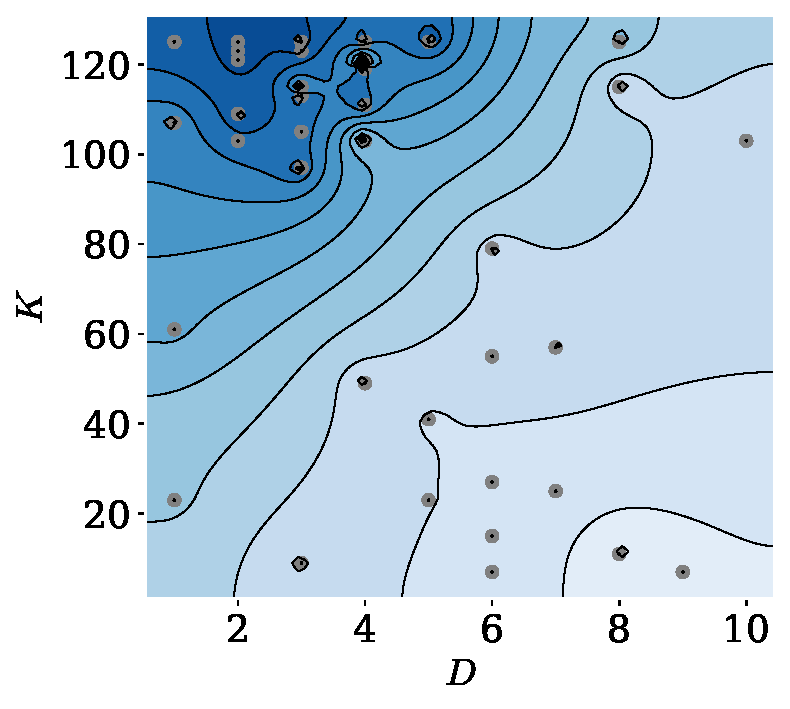
\includegraphics[width=0.33\linewidth,height=3.4cm]{Figures/contour_D_vs_K-9.pdf}} \hfill
\subfloat[$D'$ vs. $K$]{%
  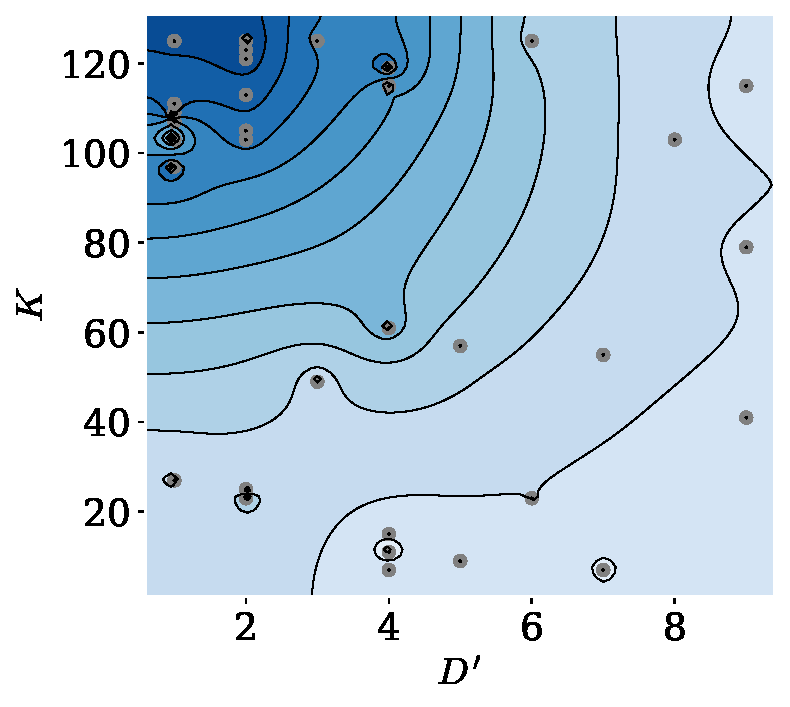
\includegraphics[width=0.33\linewidth,height=3.4cm]{Figures/contour_Dprime_vs_K-9.pdf}} \hfill
\subfloat[$D$ vs. $\mu$]{%
  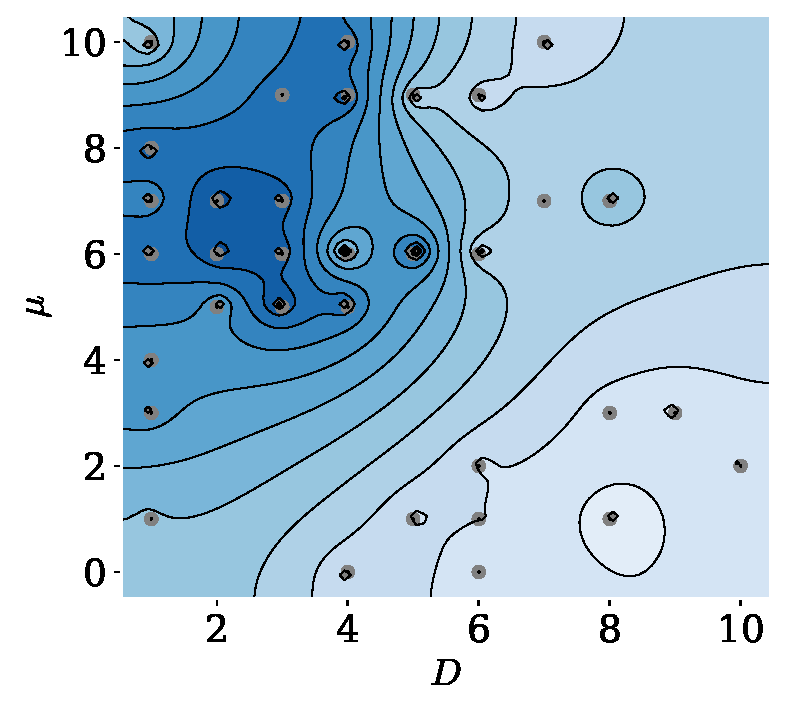
\includegraphics[width=0.33\linewidth,height=3.4cm]{Figures/contour_D_vs_mu-9.pdf}} \\[0.6em]

% --------- FILA 2 ----------
\subfloat[$D'$ vs. $\mu$]{%
  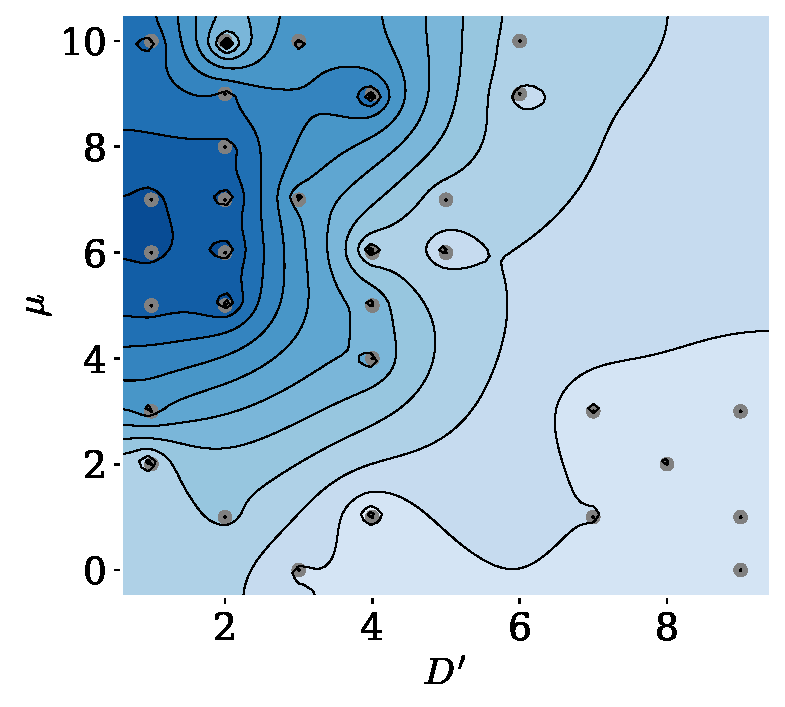
\includegraphics[width=0.33\linewidth,height=3.4cm]{Figures/contour_Dprime_vs_mu-9.pdf}} \hfill
\subfloat[$\tau$ vs. $\mu$]{%
  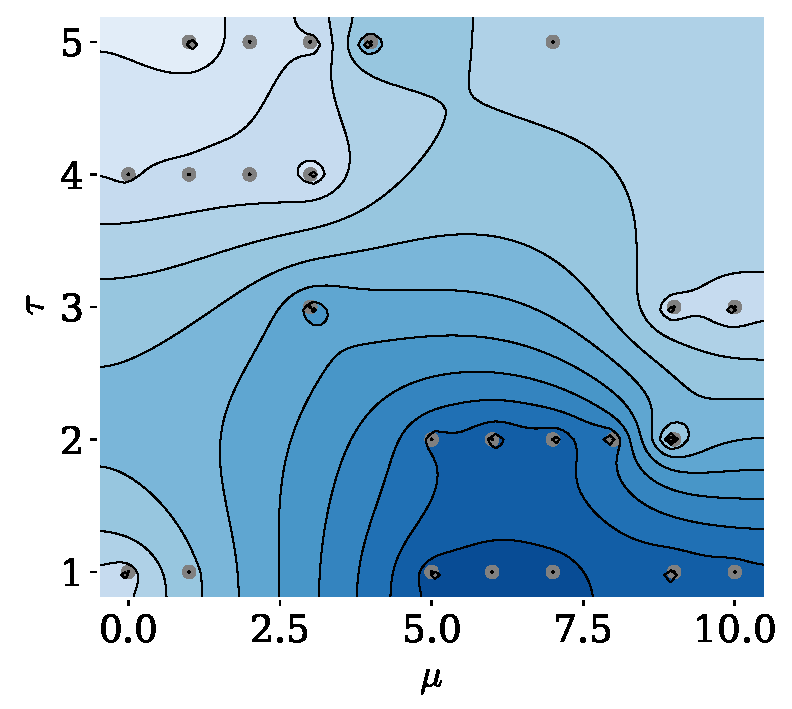
\includegraphics[width=0.33\linewidth,height=3.4cm]{Figures/contour_mu_vs_tau-9.pdf}} \hfill
\subfloat[$D'$ vs. $D$]{%
  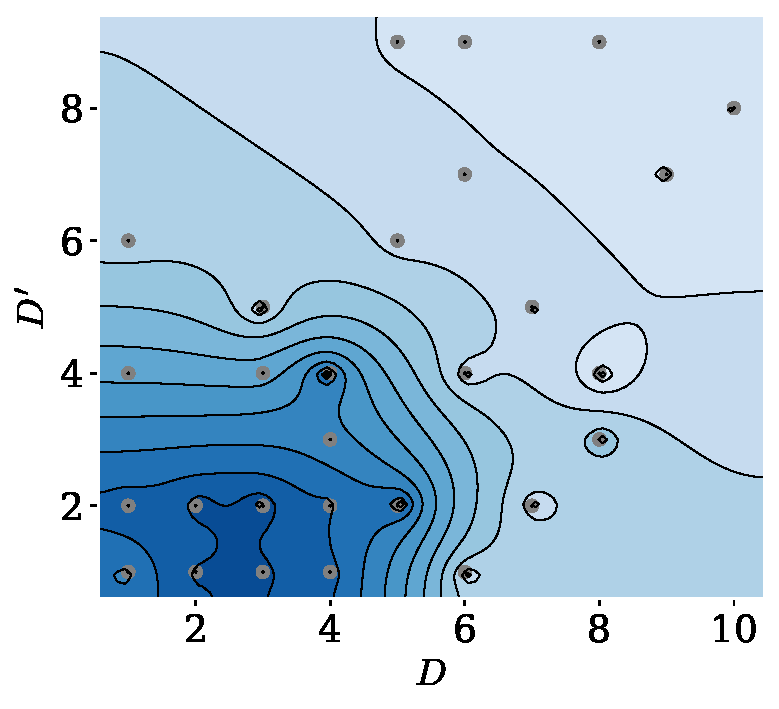
\includegraphics[width=0.33\linewidth,height=3.4cm]{Figures/contour_D_vs_Dprime-9.pdf}} \\[0.8em]

% ================= COLORBAR =================
\begin{tikzpicture}
\begin{axis}[
  hide axis,
  scale only axis,
  width=\linewidth,
  height=0pt,
  colormap name=optunablues,
  colorbar horizontal,
  point meta min=44,
  point meta max=100,
  colorbar style={
    width=\linewidth,
    height=3mm,
    xtick={44, 52, 60, 68, 76, 84, 92, 100},
    xticklabel style={font=\scriptsize},
    xlabel={val accuracy (\%)},
    xlabel style={font=\scriptsize, yshift=2pt},
    scaled ticks=false,
    /pgf/number format/fixed,
    /pgf/number format/precision=1
  }
]
\addplot[draw=none] coordinates {(0,0)};
\end{axis}
\end{tikzpicture}

\end{minipage}%
}

\caption{{Contour plots of validation accuracy (\%) as a function of selected hyperparameter pairs for the highest-performing subject (Subject~9) on the BCI Competition IV-2a dataset. All panels share the same color scale, allowing direct visual comparison across hyperparameter pairs within the subject.}}
\label{fig:global_freq_sbj9}
\end{figure}

{In contrast, for the low-performing subject (Subject~2), the contour surfaces in \Cref{fig:global_freq_sbj2} reveal a markedly less structured and more fragmented hyperparameter--performance landscape.}

%----------------------------------------------------
{For Subject~9, the contour surfaces in \Cref{fig:global_freq_sbj9} exhibit well-defined and relatively smooth high-accuracy regions, suggesting a structured optimization landscape. The panels involving the temporal kernel size $K$ show that the best validation accuracies are concentrated at large kernel values, especially when combined with low-to-moderate embedding orders $D$ and $D'$. This indicates that, for this subject, broader temporal filtering is beneficial as long as the reconstructed state-space dimensionality remains controlled. Similarly, the contours involving the interaction delay $\mu$ show favorable regions for intermediate-to-high delay values, mainly when $D$ and $D'$ remain within lower ranges. The $\mu$--$\tau$ surface further suggests that high performance is preserved for small stride values, particularly around $\tau=1$ or $\tau=2$, combined with moderate-to-large delays. Overall, Subject~9 presents compact but coherent high-performance regions, indicating that \gls{tektenet} can exploit a stable temporal-connectivity structure for this participant, provided that the temporal receptive field, delay, and embedding orders are properly balanced, which is consistent with delay-coordinate reconstruction and transfer-entropy-based modeling of nonlinear directed interactions~\cite{schreiber2000measuring}.}

%----------------------------------------------------
\begin{figure}[H]
\centering

\makebox[\textwidth][c]{%
\begin{minipage}[c]{0.99\textwidth}
\centering

% --------- FILA 1 ----------
\subfloat[$D$ vs. $K$]{%
  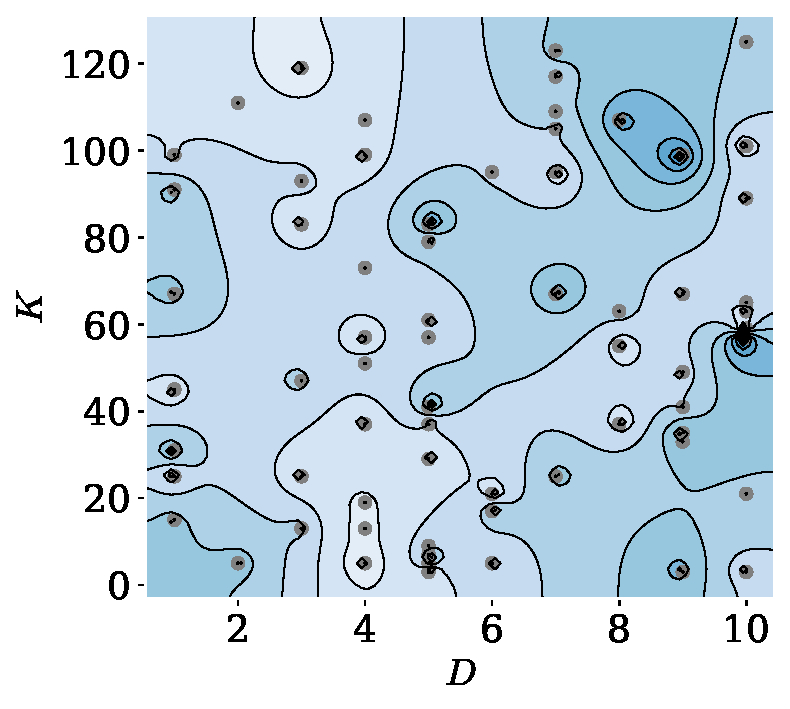
\includegraphics[width=0.33\linewidth,height=3.4cm]{Figures/contour_D_vs_K-2.pdf}} 
\subfloat[$D'$ vs. $K$]{%
  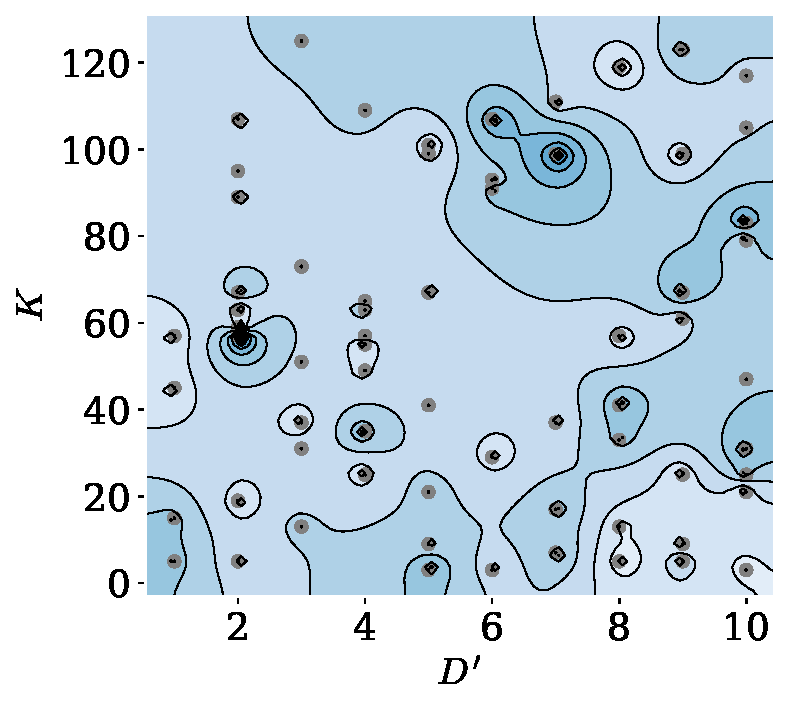
\includegraphics[width=0.33\linewidth,height=3.4cm]{Figures/contour_Dprime_vs_K-2.pdf}} 
\subfloat[$D$ vs. $\mu$]{%
  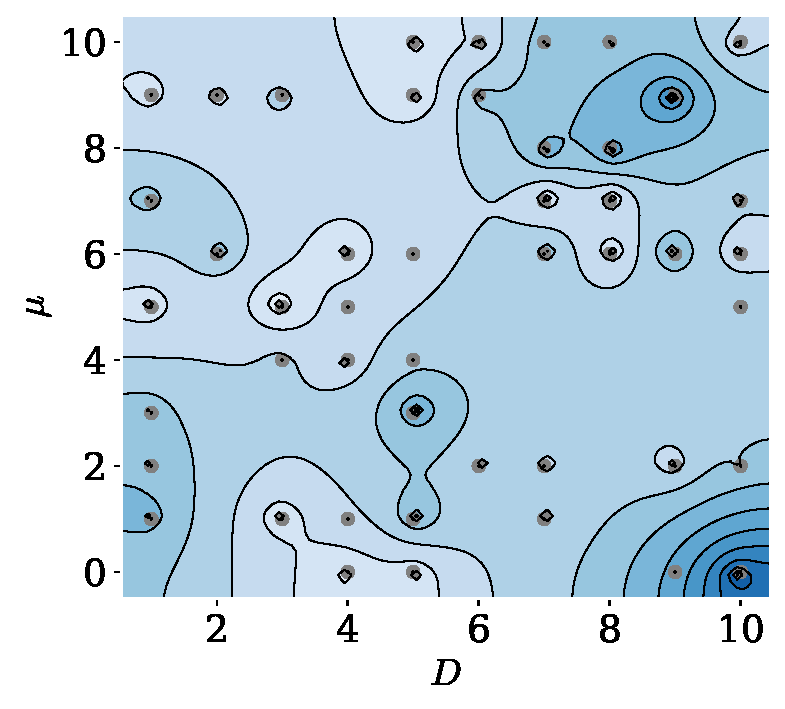
\includegraphics[width=0.33\linewidth,height=3.4cm]{Figures/contour_D_vs_mu-2.pdf}} \\[0.6em]

% --------- FILA 2 ----------
\subfloat[$D'$ vs. $\mu$]{%
  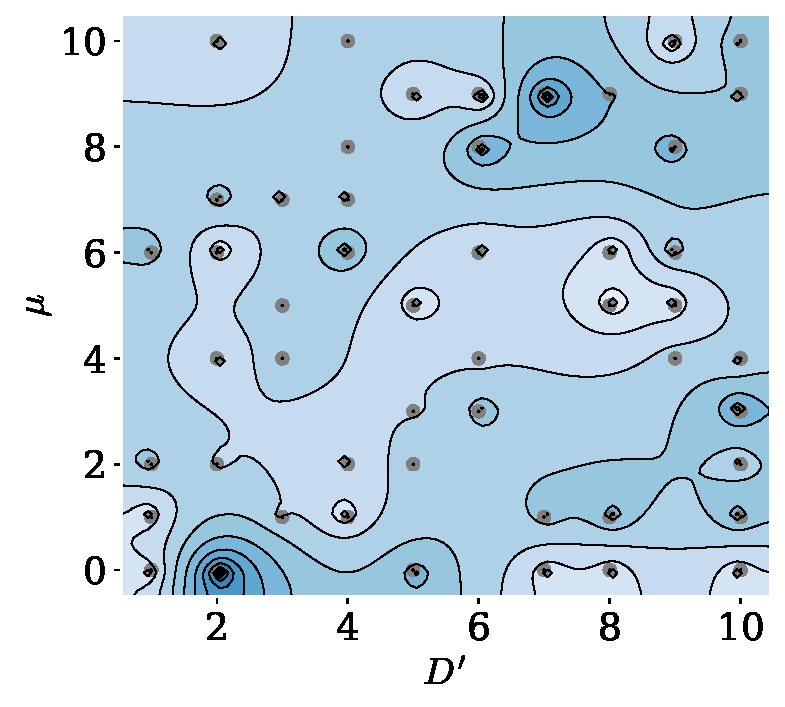
\includegraphics[width=0.33\linewidth,height=3.4cm]{Figures/contour_Dprime_vs_mu-2.pdf}} 
\subfloat[$\tau$ vs. $\mu$]{%
  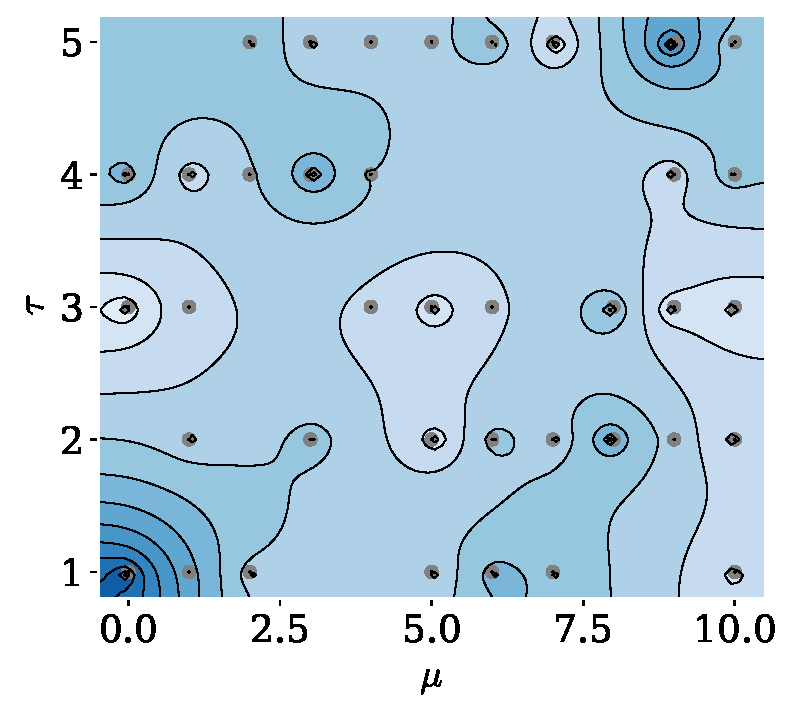
\includegraphics[width=0.33\linewidth,height=3.4cm]{Figures/contour_mu_vs_tau-2.pdf}} 
\subfloat[$D'$ vs. $D$]{%
  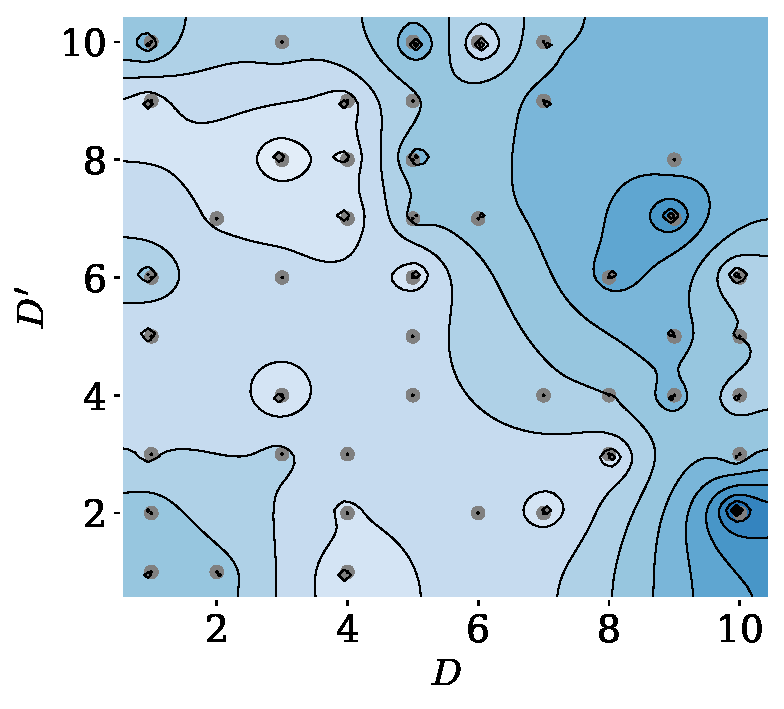
\includegraphics[width=0.33\linewidth,height=3.4cm]{Figures/contour_D_vs_Dprime-2.pdf}} \\[0.8em]

% ================= COLORBAR =================
\begin{tikzpicture}
\begin{axis}[
  hide axis,
  scale only axis,
  width=\linewidth,
  height=0pt,
  colormap name=optunablues,
  colorbar horizontal,
  point meta min=48,
  point meta max=69,
  colorbar style={
    width=\linewidth,
    height=3mm,
    xtick={48, 51, 54, 57, 60, 63, 66, 69},
    xticklabel style={font=\scriptsize},
    xlabel={val accuracy (\%)},
    xlabel style={font=\scriptsize, yshift=2pt},
    scaled ticks=false,
    /pgf/number format/fixed,
    /pgf/number format/precision=1
  }
]
\addplot[draw=none] coordinates {(0,0)};
\end{axis}
\end{tikzpicture}

\end{minipage}%
}

\caption{{Contour plots of validation accuracy (\%) as a function of selected hyperparameter pairs for the lowest-performing subject (Subject~2) on the BCI Competition IV-2a dataset. All panels share the same color scale, allowing direct visual comparison across hyperparameter pairs within the subject.}}
\label{fig:global_freq_sbj2}
\end{figure}
%----------------------------------------------------

{Unlike Subject~9, where high-accuracy regions appear more coherent and localized within specific parameter ranges, Subject~2 exhibits scattered regions of moderate performance distributed across the search space, with no clearly dominant high-performance plateau. This behavior is particularly evident in the panels involving the temporal kernel size $K$, where validation accuracy does not consistently improve for a specific range of kernel values, suggesting that broader temporal filtering alone is not sufficient to stabilize the decoding performance for this subject. Similarly, the contours involving $\mu$, $D$, and $D'$ show abrupt transitions between neighboring regions, indicating that small variations in the interaction delay or embedding dimensionality can substantially modify the reconstructed state-space representation. The $\mu$--$\tau$ surface also presents isolated regions of improved accuracy, reinforcing the idea that the temporal alignment between delayed coordinates is less stable for this participant. Overall, Subject~2 exhibits a less organized optimization landscape, consistent with its lower decoding performance and suggesting that \gls{tektenet} has greater difficulty extracting stable and discriminative temporal-connectivity patterns for this subject. This behavior is aligned with previous reports on inter-subject variability and BCI illiteracy in motor-imagery decoding~\cite{roy2020deep,ashburner2011multivariate}.}
%----------------------------------------------------
\begin{figure}[H]
    \centering
    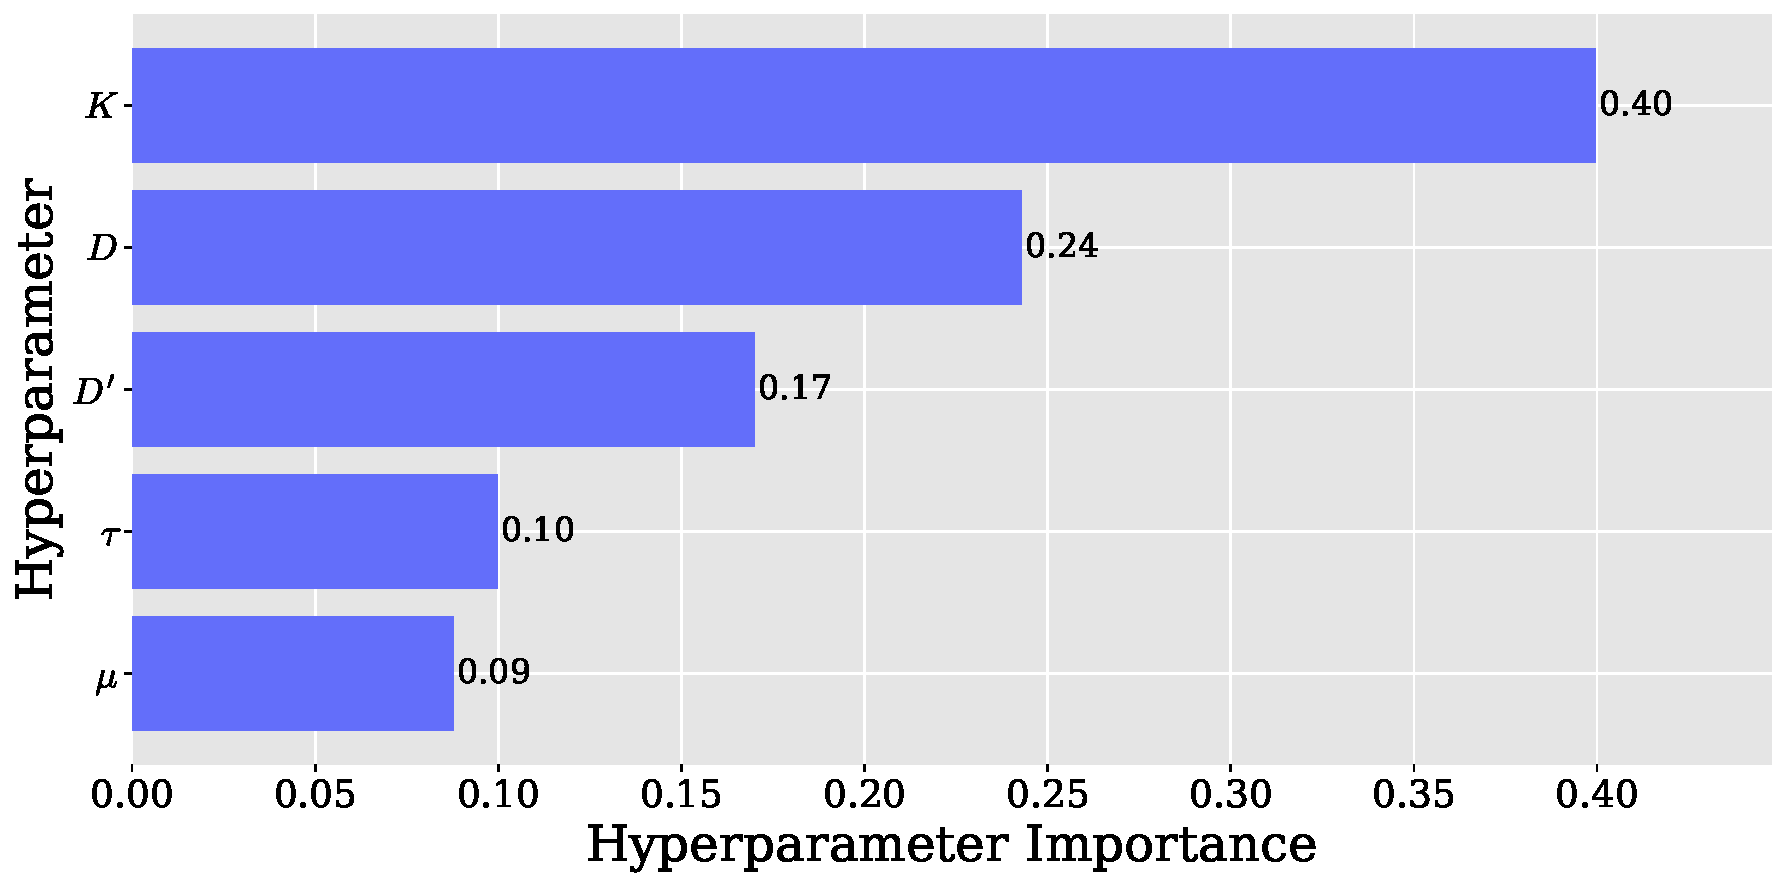
\includegraphics[width=0.8\linewidth]{Figures/optuna_fanova_param_importances_tekte-bci2a.pdf}
    \caption{{Global hyperparameter importance analysis for \gls{tektenet} on the BCI Competition IV-2a dataset. Importance scores quantify the relative contribution of the temporal kernel size $K$, embedding orders $D$ and $D'$, stride $\tau$, and interaction delay $\mu$ to validation accuracy.}}
    \label{fig:fanova_tekte_bci2a}
\end{figure}
%----------------------------------------------------
{To complement the subject-specific contour analysis, a global hyperparameter-importance analysis was conducted to quantify the relative contribution of each \gls{tektenet} hyperparameter to validation accuracy across the explored configurations. As shown in \Cref{fig:fanova_tekte_bci2a}, the temporal convolutional kernel size $K$ exhibits the highest importance score, indicating that the temporal receptive field is the dominant factor influencing model performance on the BCI Competition IV-2a dataset. This result suggests that the ability of \gls{tektenet} to extract informative temporal patterns before the Takens embedding stage is critical for subsequent directed-connectivity estimation.}

{The embedding orders also play an important role, with $D$ and $D'$ ranking as the second and third most influential hyperparameters, respectively. This finding indicates that the dimensionality of the reconstructed state space has a substantial effect on decoding performance, since it determines how much past information from the driving and responding channels is incorporated into the transfer entropy estimation~\cite{schreiber2000measuring}. In contrast, the stride $\tau$ and the interaction delay $\mu$ show lower global importance scores. However, this does not imply that these parameters are irrelevant; rather, their effects appear to be more localized and interaction-dependent, as observed in the contour plots and OAT analysis. Overall, these results indicate that \gls{tektenet} performance is mainly governed by the temporal filtering scale and the Takens embedding dimensionality, while delay and stride contribute more subtly by modulating temporal alignment between reconstructed trajectories, which is consistent with delay-coordinate reconstruction and transfer-entropy-based modeling of nonlinear directed interactions~\cite{Vicente2011,faes2011information}.}

\subsubsection{Interpretability Analysis}

For assessing model interpretability, a subject-specific analysis was conducted across temporal, spatial, and spectral axes. The temporal analysis employs a sliding-window approach for understanding time engagement and training/testing variations. On the spatial axis, the activated TE aims at interpreting functional connectivity patterns. The spectral analysis of channel-wise learned filters focuses on understanding frequency specialization. All analyses were performed under the optimized hyperparameters summarized in~\Cref{tab:hyperparameters_sorted}.

Sliding window analysis enables the exploration of MI engagement variability by examining the temporal evolution of classification accuracy. \Cref{fig:accuracy_all_subjects} presents the attained accuracy as a two-second window is slid along the trials (from 0 to 7 seconds), with subjects sorted according to their performance in~\Cref{fig:accuracy_r3}. At first glance, consistent peak classification accuracies appear within the time window between 2 and 4 seconds after the task onset. Previous studies have demonstrated that this window range suitably captures the most discriminative MI-related patterns by effectively reflecting the {temporal evolution of MI-related sensorimotor rhythms during the active motor-imagery period}~\cite{Gaur2021SlidingWindowCSP}.

  %-------------------------------------------------------------
\setlength\figurewidth{0.38\columnwidth}
\setlength\figureheight{0.3\columnwidth}
\begin{figure}[ht!]
  \centering
  %-------------------------------------------------------------
  \subfloat[\centering Subject 9]{\begin{tikzpicture}
      \begin{axis}[
        width=\figurewidth,
        height=\figureheight,
        ylabel={Accuracy (\%)},
        xlabel={Time window center ($s$)},
        xmin=1, xmax=11, ymin=30, ymax=100,
        xtick={1,...,11},
        xticklabels={1,1.5,2,2.5,3,3.5,4,4.5,5,5.5,6},
        tick pos=bottom,     
        tick label style={font=\footnotesize},
        xlabel style={font=\footnotesize},
        ylabel style={font=\footnotesize},
        minor tick num=0,
        legend style={at={(0.97,0.03)},anchor=south east,font=\footnotesize},
        legend cell align=left,
      ]
       
        \addplot[
          tabblue,
          mark=*,
          mark options={draw=tabblue,fill=tabblue},
          thick,
        ] coordinates {
          (1,58.62) (2,56.03) (3,63.79) (4,82.76) (5,99.14)
          (6,97.41) (7,84.48) (8,57.76) (9,50.00) (10,48.28)
          (11,43.10)
        };
        % \addlegendentry{Training}
        \addplot[
          taborange,
          mark=*,
          mark options={draw=taborange,fill=taborange},
          thick,
        ] coordinates {
          (1,50.00) (2,47.69) (3,51.54) (4,61.54) (5,87.69)
          (6,83.85) (7,84.62) (8,75.38) (9,72.31) (10,70.00)
          (11,62.31)
        };
        % \addlegendentry{Test}
      \end{axis}
    \end{tikzpicture}}
  \subfloat[\centering Subject 8]{    \begin{tikzpicture}
      \begin{axis}[
        width=\figurewidth,
        height=\figureheight,
        % ylabel={Accuracy (\%)},
        yticklabels=\empty,
        xlabel={Time window center ($s$)},
        xmin=1, xmax=11, ymin=30, ymax=100,
        xtick={1,...,11},
        xticklabels={1,1.5,2,2.5,3,3.5,4,4.5,5,5.5,6},
        tick pos=bottom, 
        tick label style={font=\footnotesize},
        xlabel style={font=\footnotesize}, ylabel style={font=\footnotesize},
        minor tick num=1,
        minor tick num=0,
        legend style={at={(0.97,0.03)},anchor=south east,font=\footnotesize},
        legend cell align=left,
      ]
        \addplot[
          tabblue,
          mark=*,
          mark options={draw=tabblue,fill=tabblue},
          thick,
        ] coordinates {
          (1,53.03) (2,55.30) (3,73.48) (4,89.39) (5,99.00)
          (6,94.70) (7,85.61) (8,78.03) (9,77.27) (10,73.48)
          (11,65.91)
        };
        % \addlegendentry{Training}
         \addplot[
          taborange,
          mark=*,
          mark options={draw=taborange,fill=taborange},
          thick,
        ] coordinates {
          (1,50.75) (2,47.01) (3,68.66) (4,81.34) (5,91.79)
          (6,88.81) (7,79.85) (8,76.12) (9,70.15) (10,67.91)
          (11,58.96)
        };
        % \addlegendentry{Test}
      \end{axis}
    \end{tikzpicture}}
  \subfloat[\centering Subject 3]{    \begin{tikzpicture}
      \begin{axis}[
        width=\figurewidth,
        height=\figureheight,
        % ylabel={Accuracy (\%)},
        yticklabels=\empty,
        xlabel={Time window center ($s$)},
        xmin=1, xmax=11, ymin=30, ymax=100,
        xtick={1,...,11},
        xticklabels={1,1.5,2,2.5,3,3.5,4,4.5,5,5.5,6},
        tick pos=bottom, 
        tick label style={font=\footnotesize},
        xlabel style={font=\footnotesize}, ylabel style={font=\footnotesize},
        minor tick num=1,
        minor tick num=0,
        legend style={at={(0.97,0.03)},anchor=south east,font=\footnotesize},
        legend cell align=left,
      ]
        \addplot[
          tabblue,
          mark=*,
          mark options={draw=tabblue,fill=tabblue},
          thick,
        ] coordinates {
          (1, 51.82) (2, 56.93) (3, 64.23) (4, 76.64) (5, 94.16) 
          (6, 89.05) (7, 91.97) (8, 85.40) (9, 81.75) (10, 78.10) 
          (11, 75.91)
        };
        % \addlegendentry{Training}
         \addplot[
          taborange,
          mark=*,
          mark options={draw=taborange,fill=taborange},
          thick,
        ] coordinates {
          (1, 51.82) (2, 59.85) (3, 64.96) (4, 76.64) (5, 90.51) 
          (6, 90.51) (7, 84.67) (8, 82.48) (9, 72.99) (10, 76.64) 
          (11, 67.88)
        };
        % \addlegendentry{Test}
      \end{axis}
    \end{tikzpicture}}\\
  %-------------------------------------------------------------
  \subfloat[\centering Subject 1]{    \begin{tikzpicture}
      \begin{axis}[
        width=\figurewidth,
        height=\figureheight,
        ylabel={Accuracy (\%)},
        % yticklabels=\empty,
        xlabel={Time window center ($s$)},
        xmin=1, xmax=11, ymin=30, ymax=100,
        xtick={1,...,11},
        xticklabels={1,1.5,2,2.5,3,3.5,4,4.5,5,5.5,6},
        tick pos=bottom,
        tick label style={font=\footnotesize},
        xlabel style={font=\footnotesize}, ylabel style={font=\footnotesize},
        minor tick num=1,
        minor tick num=0,
        legend style={at={(0.97,0.03)},anchor=south east,font=\footnotesize},
        legend cell align=left,
      ]
        \addplot[
          tabblue,
          mark=*,
          mark options={draw=tabblue,fill=tabblue},
          thick,
        ] coordinates {
          (1,47.37) (2,52.63) (3,81.20) (4,86.47) (5,90.98)
          (6,78.20) (7,66.17) (8,54.14) (9,54.89) (10,53.38)
          (11,51.13)
        };
        % \addlegendentry{Training}
        \addplot[
          taborange,
          mark=*,
          mark options={draw=taborange,fill=taborange},
          thick,
        ] coordinates {
          (1,52.14) (2,50.71) (3,58.57) (4,62.86) (5,62.86)
          (6,57.14) (7,52.14) (8,46.43) (9,54.29) (10,45.71)
          (11,55.00)
        };
        % \addlegendentry{Test}
      \end{axis}
    \end{tikzpicture}
}
  \subfloat[\centering Subject 7]{    \begin{tikzpicture}
      \begin{axis}[
        width=\figurewidth,
        height=\figureheight,
        % ylabel={Accuracy (\%)},
        yticklabels=\empty,
        xlabel={Time window center ($s$)},
        xmin=1, xmax=11, ymin=30, ymax=100,
        xtick={1,...,11},
        xticklabels={1,1.5,2,2.5,3,3.5,4,4.5,5,5.5,6},
        tick pos=bottom, 
        tick label style={font=\footnotesize},
        xlabel style={font=\footnotesize}, ylabel style={font=\footnotesize},
        minor tick num=1,
        minor tick num=0,
        legend style={at={(0.97,0.03)},anchor=south east,font=\footnotesize},
        legend cell align=left,
      ]
        \addplot[
          tabblue,
          mark=*,
          mark options={draw=tabblue,fill=tabblue},
          thick,
        ] coordinates {
          (1,52.17) (2,47.83) (3,68.84) (4,80.43) (5,92.75)
          (6,78.99) (7,65.22) (8,62.32) (9,57.97) (10,62.32)
          (11,55.80)

        };
        % \addlegendentry{Training}
        \addplot[
          taborange,
          mark=*,
          mark options={draw=taborange,fill=taborange},
          thick,
        ] coordinates {
         (1,45.39) (2,46.10) (3,65.25) (4,71.63) (5,77.30)
         (6,70.92) (7,66.67) (8,63.83) (9,59.57) (10,62.41)
         (11,59.57)
          
        };
        % \addlegendentry{Test}
      \end{axis}
    \end{tikzpicture}
}
  \subfloat[\centering Subject 5]{    \begin{tikzpicture}
      \begin{axis}[
        width=\figurewidth,
        height=\figureheight,
        % ylabel={Accuracy (\%)},
        yticklabels=\empty,
        xlabel={Time window center ($s$)},
        xmin=1, xmax=11, ymin=30, ymax=100,
        xtick={1,...,11},
        xticklabels={1,1.5,2,2.5,3,3.5,4,4.5,5,5.5,6},
        tick pos=bottom, 
        tick label style={font=\footnotesize},
        xlabel style={font=\footnotesize}, ylabel style={font=\footnotesize},
        minor tick num=1,
        minor tick num=0,
        legend style={at={(0.97,0.03)},anchor=south east,font=\footnotesize},
        legend cell align=left,
      ]
        \addplot[
          tabblue,
          mark=*,
          mark options={draw=tabblue,fill=tabblue},
          thick,
        ] coordinates {
          (1,52.71) (2,53.49) (3,53.49) (4,53.49) (5,96.90)
          (6,54.26) (7,58.14) (8,58.14) (9,53.49) (10,51.94)
          (11,48.84)
        };
        % \addlegendentry{Training}
        \addplot[
          taborange,
          mark=*,
          mark options={draw=taborange,fill=taborange},
          thick,
        ] coordinates {
         (1,48.15) (2,52.59) (3,40.74) (4,51.11) (5,65.93)
         (6,54.81) (7,51.11) (8,48.89) (9,45.19) (10,45.93)
         (11,48.15)
        };
        % \addlegendentry{Test}
      \end{axis}
    \end{tikzpicture}}\hfill
  %-------------------------------------------------------------
  \subfloat[\centering Subject 4]{    \begin{tikzpicture}
      \begin{axis}[
        width=\figurewidth,
        height=\figureheight,
        % ylabel={Accuracy (\%)},
        ylabel={Accuracy (\%)},
        xlabel={Time window center ($s$)},
        xmin=1, xmax=11, ymin=30, ymax=100,
        xtick={1,...,11},
        xticklabels={1,1.5,2,2.5,3,3.5,4,4.5,5,5.5,6},
        tick pos=bottom, 
        tick label style={font=\footnotesize},
        xlabel style={font=\footnotesize}, ylabel style={font=\footnotesize},
        minor tick num=1,
        minor tick num=0,
        legend style={at={(0.97,0.03)},anchor=south east,font=\footnotesize},
        legend cell align=left,
      ]
        \addplot[
          tabblue,
          mark=*,
          mark options={draw=tabblue,fill=tabblue},
          thick,
        ] coordinates {
          (1,41.59) (2,58.41) (3,54.87) (4,61.95) (5,94.69)
          (6,57.52) (7,46.90) (8,49.56) (9,48.67) (10,57.52)
          (11,54.87)
        };
        % \addlegendentry{Training}
        \addplot[
          taborange,
          mark=*,
          mark options={draw=taborange,fill=taborange},
          thick,
        ] coordinates {
          (1,47.22) (2,51.85) (3,43.52) (4,53.70) (5,61.11)
          (6,51.85) (7,49.07) (8,55.56) (9,58.33) (10,51.85)
          (11,51.85)
        };
        % \addlegendentry{Test}
      \end{axis}
    \end{tikzpicture}}
  \subfloat[\centering Subject 2]{    \begin{tikzpicture}
      \begin{axis}[
        width=\figurewidth,
        height=\figureheight,
        yticklabels=\empty,
        % ylabel={Accuracy (\%)},
        xlabel={Time window center ($s$)},
        xmin=1, xmax=11, ymin=30, ymax=100,
        xtick={1,...,11},
        xticklabels={1,1.5,2,2.5,3,3.5,4,4.5,5,5.5,6},
        tick pos=bottom,
        tick label style={font=\footnotesize},
        xlabel style={font=\footnotesize}, ylabel style={font=\footnotesize},
        minor tick num=1,
        minor tick num=0,
        legend style={at={(0.97,0.03)},anchor=south east,font=\footnotesize},
        legend cell align=left,
      ]
        \addplot[
          tabblue,
          mark=*,
          mark options={draw=tabblue,fill=tabblue},
          thick,
        ] coordinates {
          (1,53.49) (2,60.47) (3,64.34) (4,58.91) (5,51.94)
          (6,43.41) (7,48.06) (8,53.49) (9,51.16) (10,47.29)
          (11,48.84)
        };
        % \addlegendentry{Training}
        \addplot[
          taborange,
          mark=*,
          mark options={draw=taborange,fill=taborange},
          thick,
        ] coordinates {
          (1,49.14) (2,45.69) (3,52.59) (4,55.17) (5,64.66)
          (6,55.17) (7,50.00) (8,56.03) (9,52.59) (10,51.72)
          (11,46.55)
        };
        % \addlegendentry{Test}
      \end{axis}
    \end{tikzpicture}}
  \subfloat[\centering Subject 6]{    \begin{tikzpicture}
      \begin{axis}[
        width=\figurewidth,
        height=\figureheight,
        yticklabels=\empty,
        xlabel={Time window center ($s$)},
        xmin=1, xmax=11, ymin=30, ymax=100,
        xtick={1,...,11},
        xticklabels={1,1.5,2,2.5,3,3.5,4,4.5,5,5.5,6},
        tick pos=bottom,
        tick label style={font=\footnotesize},
        xlabel style={font=\footnotesize}, 
        ylabel style={font=\footnotesize},
        minor tick num=1,
        minor tick num=0,
        legend style={anchor=north east,font=\footnotesize},
        legend cell align=left,
      ]
        \addplot[
          tabblue,
          mark=*,
          mark options={draw=tabblue,fill=tabblue},
          thick,
        ] coordinates {
          (1,44.12) (2,50.00) (3,52.21) (4,53.68) (5,59.56)
          (6,52.21) (7,50.00) (8,46.32) (9,49.26) (10,49.26)
          (11,49.26)
        };
        \addlegendentry{Training}
         \addplot[
         taborange,
          mark=*,
          mark options={draw=taborange,fill=taborange},
          thick,
        ] coordinates {
          (1,52.82) (2,50.70) (3,56.34) (4,59.86) (5,61.97)
          (6,57.75) (7,54.93) (8,50.70) (9,53.52) (10,47.89)
          (11,43.66)
        };
        \addlegendentry{Test}
      \end{axis}
    \end{tikzpicture}
}
  %-------------------------------------------------------------
  \caption{Classification accuracy for each subject across overlapping time windows during the 7-second \gls{mi} task. A total of 11 time windows were used, each with a 0.5-second overlap. The x-axis represents the center of each time window, and the y-axis shows the classification accuracy (\%). This analysis reveals temporal dynamics in classification performance throughout the \gls{mi} period.}
  \label{fig:accuracy_all_subjects}
\end{figure}
%-------------------------------------------------------------

Furthermore, the temporal performance profiles cluster subjects into three groups. In the group of high-performing subjects (Subjects 9, 8, and 3), \gls{tektenet} exhibited a marked and consistent increase in accuracy of over $90\%$ within the 2–4 second window. Despite the slight decline towards the trial end, the proposed model maintained relatively high test accuracy levels (above $60\%$), suggesting the presence of stable and task-relevant neural activity in these subjects. On subjects 7, 1, and 5 (mid-performing), the proposed model performed moderately, with test accuracy peaking between $60\%$ and $80\%$ within the 2- and 4-second windows. The temporal profile of this group exhibits a clear training-to-test accuracy gap, followed by a gradual decline in training accuracy. Such a profile indicates existing MI-related neural patterns, but these are less consistent and more susceptible to cognitive variability than those in the high-performing group~\cite{duang}. For the group of low-performing subjects (Subjects 6, 4, and 2), the accuracy evolved flatly or with high variability around the chance level (between $45\%$ and $60\%$). Particularly, {Subject~4} presented severe overfitting characterized by an abrupt difference between training and test subsets in the window centered at three seconds. Such an accuracy gap is a symptom of inconsistent or weak MI-related neural patterns, which limit the reliability of classification. Therefore, the temporal performance profiles revealed differences in the quality and steadiness of the neural patterns among subjects, proving the need for subject-dependent MI models.
% %------------------------------------------------------------------------------
\begin{figure}[H]
    \centering
    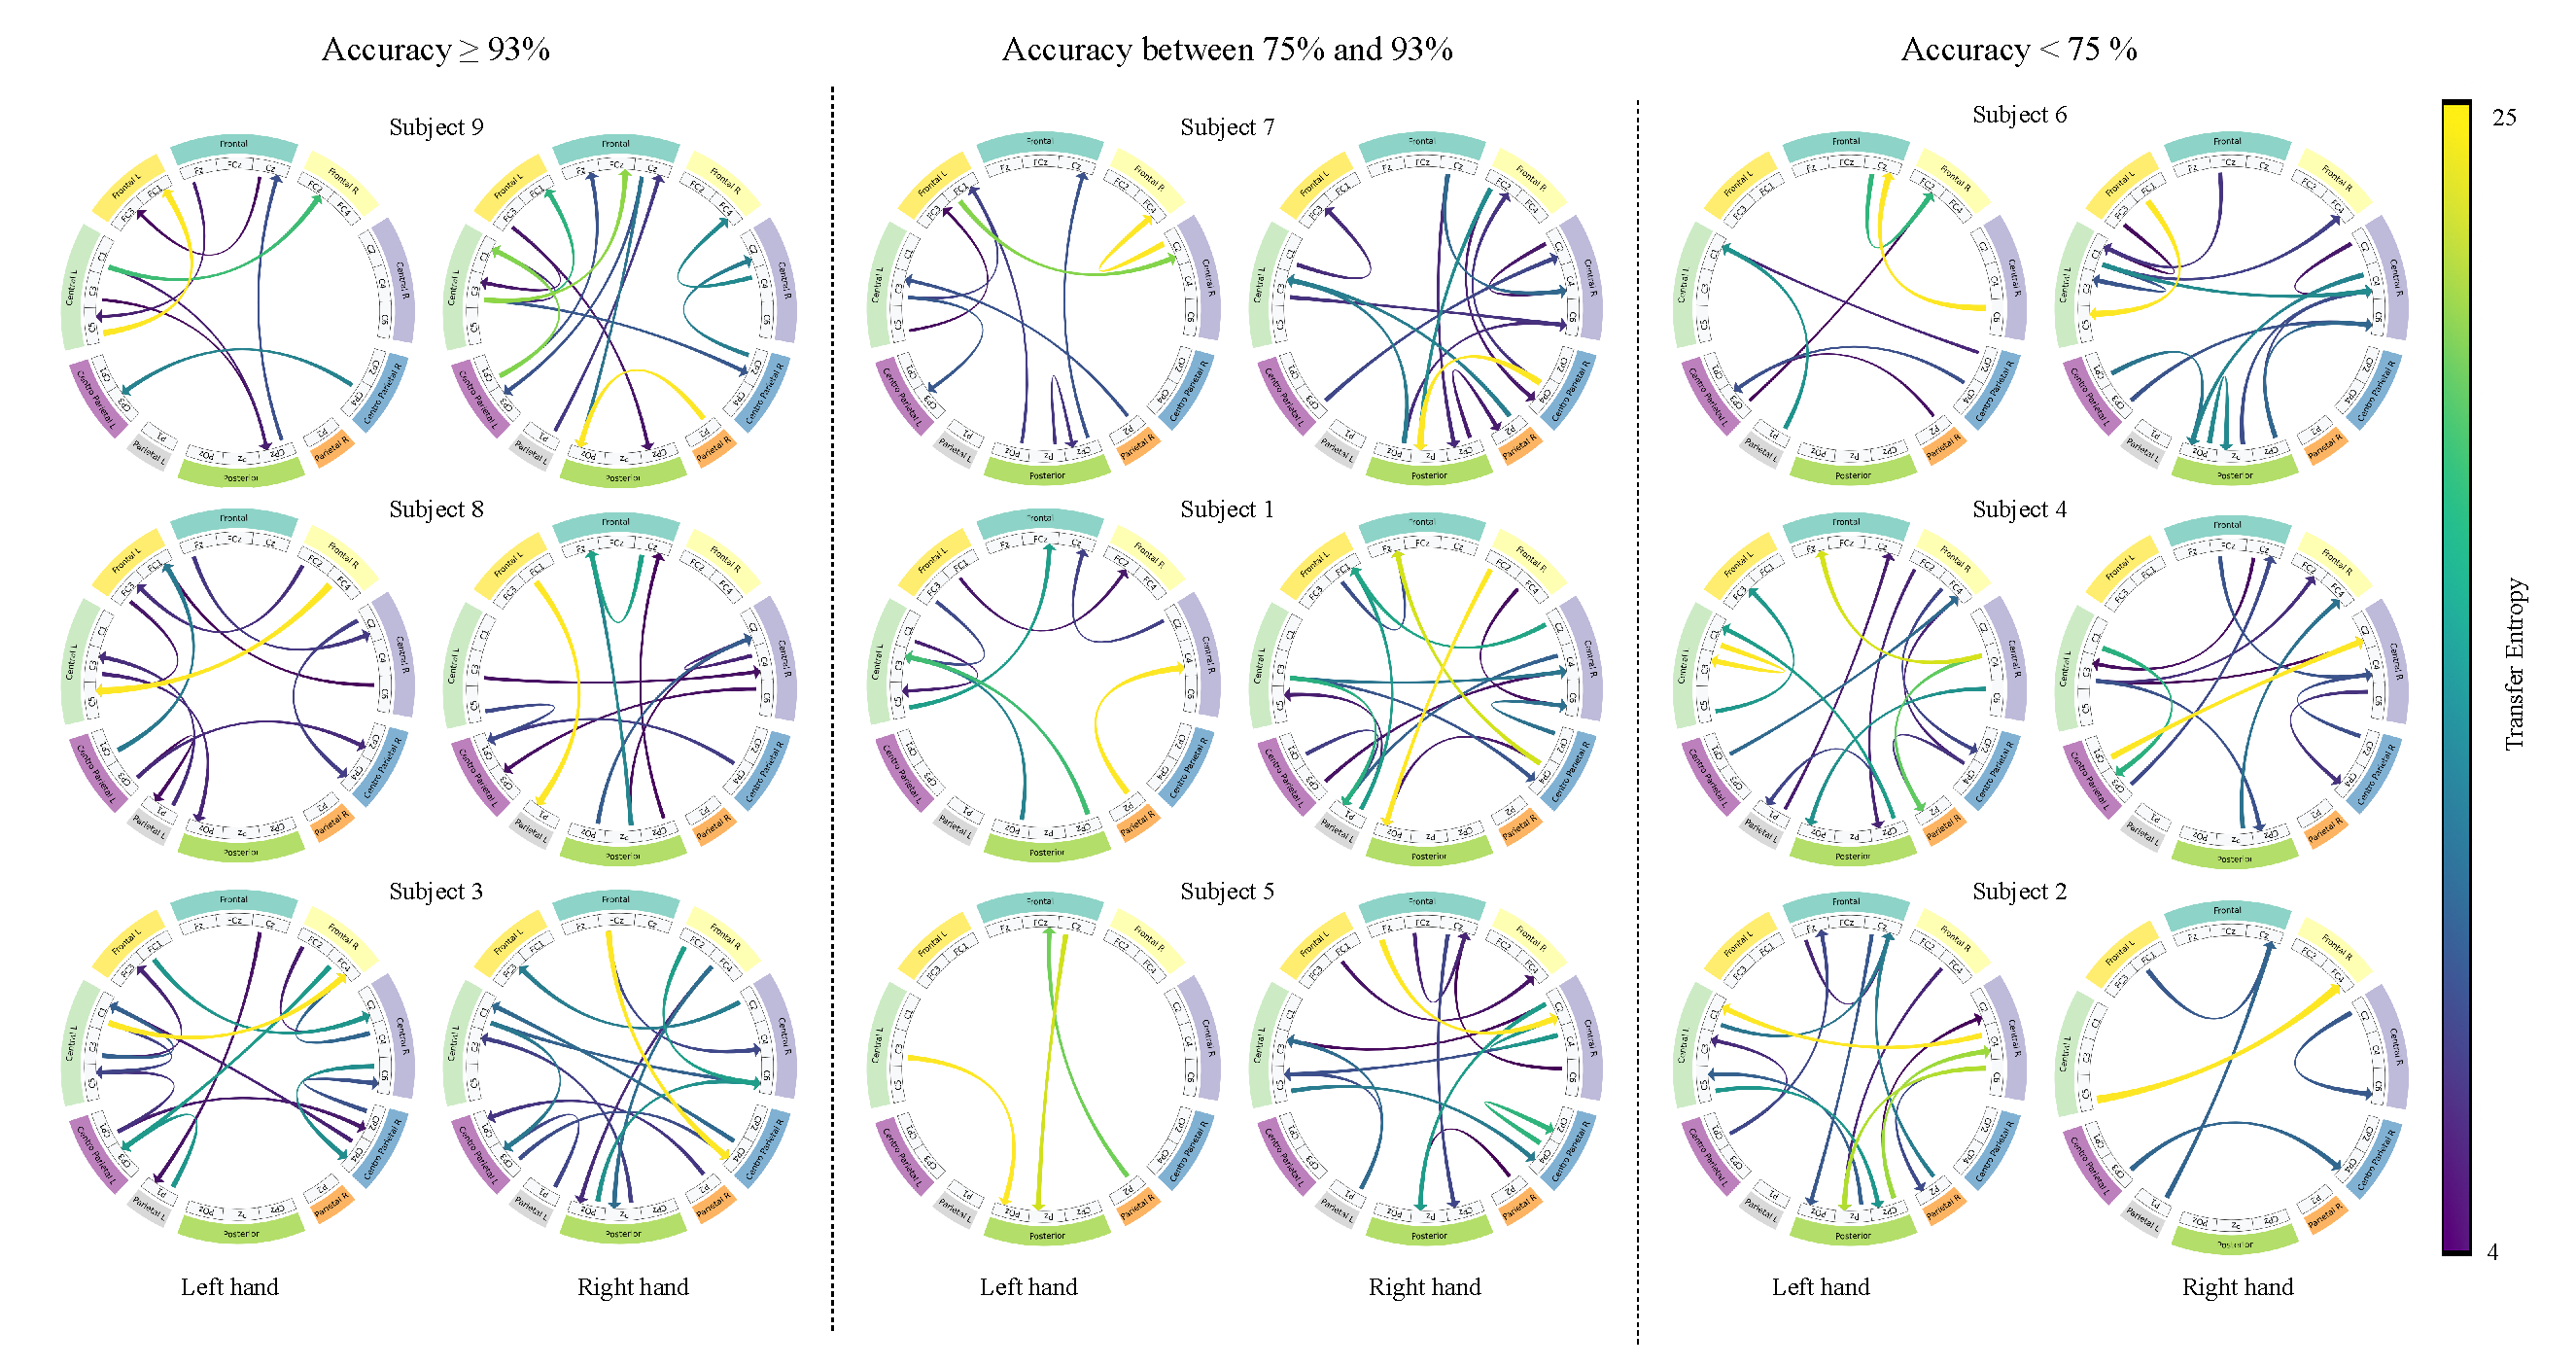
\includegraphics[width=\linewidth]{Figures/Conectivities.pdf}
    \caption{Brain connectivity patterns during left- and right-hand \gls{mi} tasks across models grouped by test accuracy. High performed (accuracy $\geq$ 93\%), mid performed (accuracy between 75\% and 93\%), and low performed (accuracy $<$ 75\%) display distinct activation distributions. Each row corresponds to a representative model within each performed group.}
    \label{fig:conectivitie}
\end{figure}
% %------------------------------------------------------------------------------
For spatial interpretability, the well-established activation maximization technique optimizes the model's output for each \gls{mi} class with respect to the TE layer. This interpretability technique enables the identification of \gls{tektenet} connectivities that strongly contribute to class-specific activations. It also allows for the analysis of the spatial distribution and intensity of interactions between brain regions, providing a clear depiction of the functional dynamics underlying \gls{mi} tasks. 

% %----------------------------------------------------------------------------
\begin{figure}[H]
  \centering

  \makebox[\textwidth]{%
    % --- Columna izquierda: "Channels" ---
    \begin{minipage}[c]{0.08\textwidth}
      \centering
      \rotatebox{90}{\normalsize Channels}
    \end{minipage}%
    \hspace{0.6em}%
    % --- Bloque derecho: paneles + colorbar ---
    \begin{minipage}[c]{0.90\textwidth}
      \centering

      % --- Tamaños (CLAVE: usar \linewidth del minipage) ---
      \newlength{\FW}
      \newlength{\FH}
      \setlength{\FW}{0.32\linewidth}  % <-- 3 por fila
      \setlength{\FH}{0.20\linewidth}

      % ====== Fila 1 ======
      \subfloat[\centering Subject 9]{%
        \includegraphics[width=\FW,height=\FH,keepaspectratio]{Figures/Freqz9.pdf}%
      }\hfill
      \subfloat[\centering Subject 7]{%
        \includegraphics[width=\FW,height=\FH,keepaspectratio]{Figures/Freqz7.pdf}%
      }\hfill
      \subfloat[\centering Subject 6]{%
        \includegraphics[width=\FW,height=\FH,keepaspectratio]{Figures/Freqz6.pdf}%
      }\\[-0.3em]

      % ====== Fila 2 ======
      \subfloat[\centering Subject 8]{%
        \includegraphics[width=\FW,height=\FH,keepaspectratio]{Figures/Freqz8.pdf}%
      }\hfill
      \subfloat[\centering Subject 1]{%
        \includegraphics[width=\FW,height=\FH,keepaspectratio]{Figures/Freqz1.pdf}%
      }\hfill
      \subfloat[\centering Subject 4]{%
        \includegraphics[width=\FW,height=\FH,keepaspectratio]{Figures/Freqz4.pdf}%
      }\\[-0.3em]

      % ====== Fila 3 ======
      \subfloat[\centering Subject 3]{%
        \includegraphics[width=\FW,height=\FH,keepaspectratio]{Figures/Freqz3.pdf}%
      }\hfill
      \subfloat[\centering Subject 5]{%
        \includegraphics[width=\FW,height=\FH,keepaspectratio]{Figures/Freqz5.pdf}%
      }\hfill
      \subfloat[\centering Subject 2]{%
        \includegraphics[width=\FW,height=\FH,keepaspectratio]{Figures/Freqz2.pdf}%
      }

      \vspace{3pt}

      % --- Texto centrado como en tu figura buena ---
      {\small\bfseries Frequency [Hz]}

      \vspace{2pt}

      % ====== Colorbar (viridis, -40..0 dB) ======
      \begin{tikzpicture}
        \begin{axis}[
          hide axis,
          scale only axis,
          width=\linewidth,
          height=0pt,
          colormap/viridis,
          point meta min=-40,
          point meta max=0,
          colorbar,
          colorbar horizontal,
          colorbar sampled,
          colorbar style={
            width=0.92\linewidth,
            height=2mm,
            at={(0.5,0)}, anchor=south,
            xtick={-40,-30,-20,-10,0},
            xticklabel style={font=\scriptsize},
            xlabel={Magnitude [dB]},
            xlabel style={font=\scriptsize, yshift=2pt},
            scaled ticks=false,
          },
        ]
          \addplot [draw=none] coordinates {(0,0)};
        \end{axis}
      \end{tikzpicture}

    \end{minipage}%
  }

  \vspace{2pt}
  \caption{Frequency responses (dB) of the filters learned by the \textit{depthwise} layer. In each panel, the $x$-axis shows frequency (Hz) and the $y$-axis shows the 22 \gls{eeg}channels; the color indicates the average magnitude in dB.}
  \label{fig:frecuencies}
\end{figure}

% %----------------------------------------------------------------------------

\Cref{fig:conectivitie} highlights the directionality, magnitude, and causal nature of the 5\% largest interactions between cortical regions, computed under the \gls{te} framework, across the nine subjects grouped according to their performance in~\Cref{fig:accuracy_r3}. In the high-performing group, causal activation patterns exhibited contralateral connections involving frontal, central, and parietal areas, emphasizing the directionality and magnitude of these connections. For instance, Subject 9 revealed strong paths including $C5\rightarrow FC1$, $C3\rightarrow FCz$, and $P2\rightarrow POz$, while Subject 8 highlighted the $FC4\rightarrow C5$ and $FC1\rightarrow P1$ connections for left and right hand MI, respectively. In the mid-performing subjects, causal interactions are more widespread and less contralateralized than in the previous group, hence partially aligning with MI-related patterns. Remarkably, connections $CP4\rightarrow Fz$ and $FC2\rightarrow POz$, in Subject 1, $C3\rightarrow POz$ and $Cz\rightarrow Pz$, in Subject 5, suggest compensatory recruitment of posterior regions. Conversely, the activations in the low-performing group lack contralateral organization, with atypical interhemispheric causal connections. For instance, the connections between the left-frontal and left-central channels in Subject 6 are atypical in the MI task~\cite{almohammadi2024}. Additionally, the right hemisphere is responsible for most of the highlighted connections in Subjects 2 and 4. Therefore, the spatial and causal interpretation of \gls{tektenet} elucidates the relationship between functional connectivity and \gls{mi} decoding performance, demonstrating efficient sensorimotor integration for the task at hand in the first group~\cite{leeuwis2021functional,vidaurre2020sensorimotor} and the compensatory recruitment of posterior regions in the second group~\cite{angulo2025proficiency}.

The characterization of the spectral behavior of the \gls{tektenet} relies on the frequency response of the channel-wise learned filters for each subject. The frequency response results from the fold-averaged magnitude of the Fast Fourier Transform computed for each convolution kernel. \Cref{fig:frecuencies} presents the resulting magnitude response (in dB) along the frequency (0 to 100Hz) and the channels (from left to right), thereby visually assessing variability among the subject groups and the selectivity of the learned filters across the frequency spectrum.

According to~\Cref{fig:frecuencies}, the proposed model yields a more structured spectral pattern in the high-performing subjects (first column) than in the rest of the cohort. In particular, the filters exhibited a band-pass-like structure in Subjects 3 and 8 around 20Hz, with a slight rightward predominance in Subject 8. From a neurophysiological perspective, the beta band (20 Hz) is associated with sensorimotor coordination and exhibits contralateral lateralization to movement, particularly within the left hemisphere during motor or spatial-orienting tasks~\cite{lasaponara2020pre}. In the case of Subject 9, the filters displayed an unattenuated response around {40 Hz}, primarily concentrated {over right-hemispheric channels}. {This pattern should be interpreted cautiously as a model-derived spectral relevance rather than as direct evidence of a cortical gamma generator, since scalp EEG responses in this frequency range may be influenced by source mixing, volume conduction, residual artifacts, or myogenic contamination~\cite{Whitham2007Scalp}.} Hence, the structured frequency response suggests that the depthwise convolutional filters adapt to preserve the oscillatory components, relevant for the classification task, effectively acting as spectral selectors that maintain frequency regions containing discriminative neural information.

Regarding the second group and third groups (center and right columns), the spectral behavior was less defined compared to the first group. Only the learned filters for Subject 1 partially selected frequencies around 25 Hz over the left hemisphere, similar to the best-performed subjects, albeit with lower clarity and spatial extent. For Subjects 7 and 5, the filters develop a spurious magnitude response, lacking spectral or spatial alignment. Contrarily, the depthwise convolutional filters for the latter group yield an elongated and flat spectral response, reflecting the absence of frequency selectivity. Therefore, the \gls{tektenet}'s spectral specialization positively relates to classification performance, as the low power of MI-related rhythms, particularly beta and gamma, is associated with lower cognitive performance and reduced classification accuracy~\cite{bakhtiari2023power, avital2024cognitive}.

\subsubsection{Performance Assessment}

{This contribution evaluates} \gls{tektenet}'s performance on the official testing set from the BCI Competition IV Dataset 2a. \Cref{tab:metric_results} presents the per-subject performance metrics on this subset, sorted by validation accuracy.

In general, note that the testing accuracy naturally decreased by approximately 7\% compared to the validation one, due to the intrinsic within-subject variability. However, the average F1 score of over 80\% indicates that \gls{tektenet} successfully identified individual \gls{mi} patterns, demonstrating a reasonable generalization capability. For the high-performing group, the model consistently reached scores of over 90\%. Such a result indicates that \gls{tektenet} finds well-structured neurophysiological patterns with both precision and generalizability. For the mid-performing group, \gls{tektenet} yields F1 scores between 75\% and 85\%, followed by the most significant accuracy drops compared to the validation set. Such a finding indicates transitional signal regimes or moderate generalization characteristics, due to accentuated between-session variability. The low-performing group remains just above the chance levels, suggesting highly intrinsic neurophysiological noise or BCI illiteracy. It is also worth mentioning that Subjects 5, 4, and 2 present the most difference between Sensitivity and Specificity, with F1 scores over  65\%, despite the class balance provided by the competition. Hence, the heterogeneity in class distributions emerges as the most reasonable explanation for uneven metrics on such subjects, which facilitates the labeling of the positive class while hindering the negative. Therefore, the stratification and subject-wise analysis highlight the necessity of adaptive or personalized strategies in BCI decoding frameworks, while providing a deeper understanding of the inner workings of \gls{tektenet} across individuals. 
% %----------------------------------------------------------------------------
\begin{table}[H]
\centering
\begin{tabular}{crrrrr}
\toprule
\textbf{Subject} & \textbf{Val. Acc (\%)} & \textbf{Acc. (\%)} & \textbf{F1 (\%)} & \textbf{Sens. (\%)} & \textbf{Spec. (\%)}\\
\midrule
9 & $99.1 \pm 1.9$  & $90.0$  & $90.1$  & $90.8$  & $89.2$\\
8 & $98.5 \pm 2.0$  & $92.5$  & $92.8$  & $94.1$  & $90.9$\\
3 & $94.2 \pm 6.0$  & $93.4$  & $93.9$  & $98.6$  & $88.1$\\
7 & $91.7 \pm 6.9$  & $77.1$  & $78.7$  & $85.5$  & $69.0$\\
1 & $89.9 \pm 8.3$  & $85.1$  & $85.3$  & $87.1$  & $83.1$\\
5 & $88.4 \pm 5.1$  & $74.8$  & $75.0$  & $78.5$  & $71.4$\\
6 & $72.6 \pm 8.4$  & $73.1$  & $71.3$  & $65.5$  & $81.1$\\
4 & $72.3 \pm 13.7$ & $75.0$  & $74.8$  & $75.4$  & $74.6$\\
2 & $67.7 \pm 8.4$  & $59.9$  & $66.7$  & $80.3$  & $39.4$\\
\midrule
\textbf{Avg} & $\mathbf{86.0 \pm 2.5}$ & $\mathbf{80.1}$ & $\mathbf{81.0}$ & $\mathbf{84.0}$ & $\mathbf{76.3}$\\
\bottomrule
\end{tabular} 
\caption{Performance metrics achieved by \gls{tektenet} on the validation and official testing sets. Subjects are sorted in descending order of validation accuracy. Mean and standard deviation for each metric are computed from a five-fold cross-validation.}
\label{tab:metric_results}
\end{table}
%-----------------------------------------------

\Cref{tab:acc_comparisonn} contrasts the proposed \gls{tektenet} against state-of-the-art approaches on the testing sets from the BCI Competition IV in terms of Floating Point Operations (FLOPs), number of trainable parameters (NTP), and average accuracy (color-coded). Both, FLOPs and NTP, describe the computational efficiency and complexity of models, which directly impact performance, scalability, and deployability. Contrasted approaches range from traditional feature engineering techniques (square mark), through deep learning architectures (circle mark), to hybrid models (triangle mark). The formers include time-frequency, dynamic nonlinear~\cite{Degirmenci2024,Degirmenci2023}, and entropy-based connectivity features~\cite{de2019data}, which achieved accuracies ranging from $60\%$ to $70\%$. While these methods benefit from high interpretability, they rely heavily on handcrafted statistical features and traditional classifiers. This reliance limits their ability to model the complex spatiotemporal characteristics inherent to \gls{eeg}signals, which in turn constrains their generalization capacity and scalability to diverse experimental conditions.

The seminal deep learning models, explicitly designed for \gls{eeg}decoding~\cite{lawhern2018eegnet}, introduce automated feature extraction pipelines that reach accuracies up to $68\%$. Hence, the between-session variability hampers their performance due to overfitting and a lack of inherent regularization through parameterized features. More recently, Transformer-based architectures have shown competitiveness in capturing long-range dependencies through self-attention and a global receptive field, facilitating the integration of multi-channel information. For instance, CTNet reports $88.49\pm9.03\%$ on BCI IV-2b (two classes)~\cite{CTNet}, while CNNViT attains $81.11\%$ on BCI IV-2b under a subject-independent LOSOCV protocol~\cite{CNNViT}. However, both models demand larger computational and memory resources, substantial amounts of data (or pretraining), careful hyperparameter tuning, and offer more limited neurophysiological interpretability. In turn, the \gls{tektenet} and GAT+PLV proposals introduce hybrid frameworks that integrate functional connectivity measures with deep learning architectures. In particular, GAT+PLV feeds a Graph Attention Network with Phase-Locking Value connectivity~\cite{patel2025advancing}. On the official test set, \gls{tektenet} achieves an accuracy of 80.12\%, surpassing GAT+PLV by 8.21\%, which requires the explicit precomputation of phase coupling (PLV). These findings suggest that connectivity-informed, end-to-end architectures outperform traditional deep networks and hybrid architectures, while being competitive against modern transformer-based models.

%----------------------------------------------
\begin{figure}[H]
  \centering
  % Carga y escala al 90% del ancho de texto
  \resizebox{0.8\textwidth}{!}{\tikzexternaldisable 
\begin{tikzpicture}
\pgfplotstableread[col sep=semicolon]{
method;acc;params;flops;cat
DeepConvNet (2017);67.62;1.70e5;1.30e7;cnn
ShallowConvNet (2017);66.41;5.00e4;9.00e6;cnn
EEGNet (2018);65.49;1.80e3;9.30e5;cnn
TE$\kappa_\alpha$ (2019);68.80;3.00e1;1.39e12;features
StatFeat-Ensemble v2 (2024);63.04;1.00e2;9.00e5;features
GAT+PLV (2025);71.89;1.50e4;2.00e6;hybrid
CNNViT-MILF$^{\dagger}$ (2025);81.11;4.10e5;5.10e7;cnn
CTNet$^{\dagger}$ (2025);88.49;2.57e4;4.00e7;cnn
\textbf{TEKTE-Net (Ours)};80.12;6.95e3;3.31e7;hybrid
}\methoddata

\begin{axis}[
  width=\linewidth,
  xmode=log, ymode=log,
  log basis x=10, log basis y=10,
  xlabel={FLOPs (per trial)},
  ylabel={NTP},
  grid=both,
  minor grid style={opacity=0.1},
  major grid style={opacity=0.25},
  tick pos=bottom, tick align=inside, tick style={black!60},
  xmin=7e5, xmax=2e13,
  ymin=2e1, ymax=6e5,
  clip=false,
  colormap/viridis,
  colorbar,
  point meta min=60, point meta max=90, 
  colorbar style={ylabel=Accuracy [\%], yticklabel style={/pgf/number format/fixed}, tick pos=right,
  },
  scatter/use mapped color={draw=mapped color, fill=mapped color},
  unbounded coords=discard, 
  legend cell align={left},
  legend pos=north east,
  legend style={draw=black,
  fill=white,
  fill opacity=0.85, text opacity=1,
  font=\small},
]

\addplot[
  scatter, only marks, mark=*, mark size=3pt,
  scatter src=explicit, point meta=\thisrow{acc},
  forget plot,
]
table[
  x expr={\ifnum\pdfstrcmp{\thisrow{cat}}{cnn}=0 \thisrow{flops} \else nan \fi},
  y expr={\ifnum\pdfstrcmp{\thisrow{cat}}{cnn}=0 \thisrow{params} \else nan \fi},
  meta=acc
] {\methoddata};

\addplot[
  scatter, only marks, mark=square*, mark size=3pt,
  scatter src=explicit, point meta=\thisrow{acc},
  forget plot,
]
table[
  x expr={\ifnum\pdfstrcmp{\thisrow{cat}}{features}=0 \thisrow{flops} \else nan \fi},
  y expr={\ifnum\pdfstrcmp{\thisrow{cat}}{features}=0 \thisrow{params} \else nan \fi},
  meta=acc
] {\methoddata};

\addplot[
  scatter, only marks, mark=triangle*, mark size=3pt,
  scatter src=explicit, point meta=\thisrow{acc},
  forget plot,
]
table[
  x expr={\ifnum\pdfstrcmp{\thisrow{cat}}{hybrid}=0 \thisrow{flops} \else nan \fi},
  y expr={\ifnum\pdfstrcmp{\thisrow{cat}}{hybrid}=0 \thisrow{params} \else nan \fi},
  meta=acc
] {\methoddata};

\addlegendimage{only marks, mark=square*,   mark size=3pt, mark options={fill=gray!60,draw=black}}
\addlegendentry{Feature-based}
\addlegendimage{only marks, mark=*,        mark size=3pt, mark options={fill=gray!60,draw=black}}
\addlegendentry{DL-based}
\addlegendimage{only marks, mark=triangle*, mark size=3pt, mark options={fill=gray!60,draw=black}}
\addlegendentry{Hybrid}

\addplot[
  only marks, mark=none,
  nodes near coords, nodes near coords align={left},
  every node near coord/.style={
    font=\footnotesize, anchor=west, xshift=2pt, yshift=2pt,
    fill=white, fill opacity=0.65, text opacity=1,
    inner sep=1pt, rounded corners=1pt
  },
  point meta=explicit symbolic,
] table[x=flops, y=params, meta=method] {\methoddata};

\end{axis}
\end{tikzpicture}
\tikzexternalenable
}
  \caption{State-of-the-art comparison for binary MI-\gls{eeg}decoding in terms of Floating Point Operations (FLOPs), number of trainable parameters (NTP), and testing accuracy. $^{\dagger}$ Accuracy reported on the BCI Competition IV-2b testing set (Left vs. Right).}
  \label{tab:acc_comparisonn}
\end{figure}
%-----------------------------------------------

\subsubsection{Validation on large-scale scenarios: Subject-independent decoding on the GigaScience dataset}

To further evaluate the scalability and generalization capability of \gls{tektenet}, a subject-independent analysis was conducted on the GigaScience dataset, comprising 50 subjects. Due to the scale of this experiment, reporting the optimal hyperparameter configuration for each subject individually becomes impractical. Instead, the analysis is supported by an inter-subject accuracy comparison, shown in Fig.~\ref{fig:acc_eegnet_vs_tekte}, which summarizes the resulting performance of \gls{tektenet} after hyperparameter tuning relative to EEGNet, used here as the baseline model.

In particular, it is observed that, although \gls{tektenet} maintains or even exhibits slight decreases in accuracy for some high-performing subjects compared to EEGNet, it achieves substantial improvements for a large proportion of low-performing subjects. This behavior suggests that \gls{tektenet} is especially beneficial in scenarios where neural patterns are less separable or more affected by noise, effectively reducing the performance gap across subjects and contributing to a more homogeneous performance distribution.

\begin{figure}[htbp]
 \hspace{-12pt}\resizebox{\linewidth}{!}{%

% --------- Dimensiones y colores ----------
\def\FigW{20cm}
\def\FigH{8.5cm}

\definecolor{EEGNetDark}{HTML}{7CD8E2}
\definecolor{EEGNetLight}{HTML}{CAEBF1}
\definecolor{TEKTEDark}{HTML}{98D891}
\definecolor{TEKTELight}{HTML}{ABE3A1}

% --------- Estilos ----------
\pgfplotsset{
  myaxis/.style={
    width=\FigW, height=\FigH,
    ymin=45, ymax=101,
    ylabel={Accuracy [\%]},
    ylabel style={font=\small},
    ytick={45,50,60,70,80,90,100},
    xtick pos=bottom, ytick pos=left,
    tick align=inside,
    ticklabel style={font=\scriptsize},
    axis lines=box,
    tick style={black!60},
    xmajorgrids, ymajorgrids,
    grid style={black!15},
  },
  methodline/.style={
    line width=1.1pt,
    mark=*,
    mark size=1.6pt,
    mark options={solid, draw=#1, fill=#1},
    draw=#1
  },
  bandstyle/.style={draw=none, fill opacity=0.40},
}

% --------- Datos (ordenados por ACC EEGNet de MAYOR a MENOR) ---------
% Columnas:
% subj  eegnet(%)  eegnet_std(%)  tekte(%)  tekte_std(%)
\pgfplotstableread[row sep=\\, col sep=space]{
subj  eegnet  eegnet_std  tekte  tekte_std \\
43    99.50   0.00        93.75  0.00 \\
14    97.00   0.00        92.50  0.00 \\
3     93.50   0.00        83.75  0.00 \\
48    92.50   0.00        63.75  0.00 \\
50    92.50   0.00        67.50  0.00 \\
4     91.00   0.00        63.75  0.00 \\
35    88.00   0.00        81.25  0.00 \\
13    84.00   0.00        83.75  0.00 \\
23    84.00   0.00        73.75  0.00 \\
41    83.00   0.00        71.25  0.00 \\
1     81.00   0.00        85.00  0.00 \\
49    78.97   0.00        85.90  0.00 \\
37    77.00   0.00        92.50  0.00 \\
5     76.50   0.00        82.50  0.00 \\
26    76.50   0.00        65.00  0.00 \\
44    76.00   0.00        70.00  0.00 \\
6     75.56   0.00        80.56  0.00 \\
47    74.87   0.00        78.21  0.00 \\
28    74.50   0.00        65.00  0.00 \\
36    73.85   0.00        70.51  0.00 \\
12    72.57   0.00        72.86  0.00 \\
39    71.00   0.00        68.75  0.00 \\
46    69.17   0.00        72.91  0.00 \\
10    68.00   0.00        73.75  0.00 \\
20    64.71   0.00        85.29  0.00 \\
22    64.00   0.00        66.25  0.00 \\
31    63.00   0.00        62.50  0.00 \\
18    62.00   0.00        80.00  0.00 \\
52    61.50   0.00        71.25  0.00 \\
25    60.50   0.00        71.25  0.00 \\
21    59.00   0.00        73.75  0.00 \\
40    58.00   0.00        67.50  0.00 \\
24    57.50   0.00        75.00  0.00 \\
27    56.22   0.00        64.86  0.00 \\
30    56.00   0.00        70.00  0.00 \\
42    55.50   0.00        65.00  0.00 \\
16    55.00   0.00        68.75  0.00 \\
9     55.00   0.00        70.83  0.00 \\
38    54.87   0.00        68.75  0.00 \\
19    54.48   0.00        72.41  0.00 \\
33    54.00   0.00        68.75  0.00 \\
11    54.00   0.00        76.25  0.00 \\
2     54.00   0.00        70.00  0.00 \\
17    53.50   0.00        67.50  0.00 \\
15    53.33   0.00        64.10  0.00 \\
45    53.00   0.00        83.75  0.00 \\
32    52.00   0.00        63.75  0.00 \\
7     51.67   0.00        83.33  0.00 \\
8     50.00   0.00        75.00  0.00 \\
}\datatable

\begin{tikzpicture}
\begin{axis}[
  myaxis,
  enlarge x limits=0,
  xlabel={Subjects},
  symbolic x coords={
    43,14,3,48,50,4,35,13,23,41,
    1,49,37,5,26,44,6,47,28,36,
    12,39,46,10,20,22,31,18,52,25,
    21,40,24,27,30,42,16,9,38,19,
    33,11,2,17,15,45,32,7,8
  },
  xtick=data,
  x tick label style={rotate=90, anchor=east},
  legend style={
    at={(rel axis cs:0.001,0.001)}, anchor=south west,
    draw=black!40, fill=white, fill opacity=0.9, font=\small,
    rounded corners=2pt
  },
  legend cell align=left,
]

% ===== EEGNet (std=0) =====
\addplot[name path=EEGNetUpper, draw=none, forget plot]
  table [x=subj, y expr=\thisrow{eegnet}+\thisrow{eegnet_std}] {\datatable};
\addplot[name path=EEGNetLower, draw=none, forget plot]
  table [x=subj, y expr=\thisrow{eegnet}-\thisrow{eegnet_std}] {\datatable};
\addplot[bandstyle, fill=EEGNetLight, forget plot]
  fill between[of=EEGNetUpper and EEGNetLower];
\addplot[methodline={EEGNetDark}]
  table [x=subj, y=eegnet] {\datatable};

% ===== TEKTE-Net (std=0) =====
\addplot[name path=TEKTEUpper, draw=none, forget plot]
  table [x=subj, y expr=\thisrow{tekte}+\thisrow{tekte_std}] {\datatable};
\addplot[name path=TEKTELower, draw=none, forget plot]
  table [x=subj, y expr=\thisrow{tekte}-\thisrow{tekte_std}] {\datatable};
\addplot[bandstyle, fill=TEKTELight, forget plot]
  fill between[of=TEKTEUpper and TEKTELower];
\addplot[methodline={TEKTEDark}]
  table [x=subj, y=tekte] {\datatable};

% ===== Leyenda =====
\addlegendimage{line legend, draw=EEGNetDark, mark=*}
\addlegendentry{EEGNet}
\addlegendimage{line legend, draw=TEKTEDark, mark=*}
\addlegendentry{\gls{tektenet}}

\end{axis}
\end{tikzpicture}
}
\caption{{Inter-subject classification accuracies for EEGNet and \gls{tektenet}. Subjects are ordered according to their EEGNet accuracy.}}
\label{fig:acc_eegnet_vs_tekte}
\end{figure}
%--------------------------------------------

{To provide a more interpretable view of the hyperparameter behavior, two representative subjects were selected from the GigaScience dataset: one high-performing subject (Subject~14) and one low-performing subject (Subject~27). These subjects illustrate contrasting optimization regimes under favorable and challenging signal conditions, respectively. For these cases, contour plots were generated from the completed hyperparameter-optimization trials to examine how validation accuracy changes across selected pairs of \gls{tektenet} hyperparameters, including the temporal kernel size $K$, the embedding orders $D$ and $D'$, the stride $\tau$, and the interaction delay $\mu$. Thus, the contour analysis provides a visual approximation of the explored hyperparameter--performance landscape, allowing the identification of stable high-performing regions, as well as configurations in which the model becomes more sensitive to specific hyperparameter choices.}

{For the high-performing subject (Subject~14), the contour plots in Fig.~\ref{fig:global_freq_Giga14} reveal a relatively favorable optimization landscape, with several regions of high validation accuracy across different hyperparameter combinations. The projections involving the temporal kernel size $K$ and the embedding dimensions ($D$, $D'$) suggest that high performance can be achieved for multiple configurations, particularly when the temporal receptive field and the reconstructed state-space dimensionality are properly balanced. However, the surfaces also show localized variations, indicating that performance is not completely insensitive to the choice of hyperparameters.}

{The interactions involving the delay parameter $\mu$ show that favorable performance can be maintained over several delay values, especially when combined with suitable embedding dimensions. Nevertheless, the presence of localized peaks and transitions suggests that the estimation of delayed directed dependencies still depends on an appropriate alignment among $\mu$, $\tau$, and the embedding parameters, which is consistent with the sensitivity of nonlinear directed-dependency estimation to temporal embedding choices~\cite{schreiber2000measuring,staniek2008symbolic}. Similarly, the $D$--$D'$ projection does not indicate a single isolated optimum, but rather a set of effective configurations in which the embedding space can be constructed flexibly within an adequate range. Overall, these results suggest that Subject~14 represents a favorable optimization regime for \gls{tektenet}, where discriminative temporal-connectivity patterns can be captured without requiring an extremely restrictive hyperparameter configuration.}
%----------------------------------------------------
\begin{figure}[H]
\centering

% ---------- Tamaños ----------
\setlength{\FW}{0.34\linewidth}
\setlength{\FH}{3.4cm}

\makebox[\textwidth][c]{%

% ================= PANEL 3x2 + COLORBAR =================
\begin{minipage}[c]{0.99\textwidth}
\centering

% --------- FILA 1 ----------
\subfloat[$D$ vs. $K$]{%
  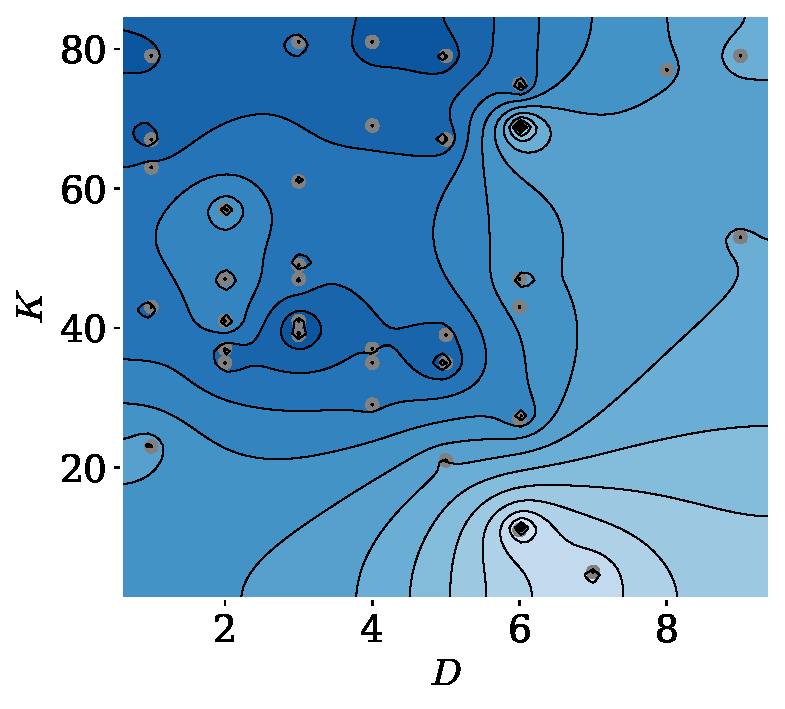
\includegraphics[width=\FW,height=\FH]{Figures/contour_D_vs_K-14.pdf}} 
\subfloat[$D'$ vs. $K$]{%
  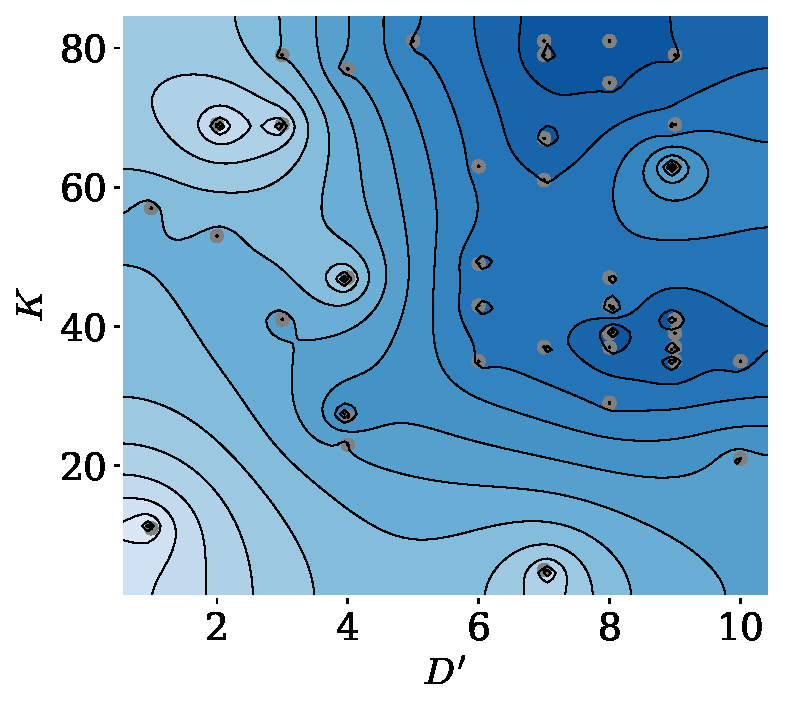
\includegraphics[width=\FW,height=\FH]{Figures/contour_Dprime_vs_K-14.pdf}} 
\subfloat[$D$vs. $\mu$]{%
  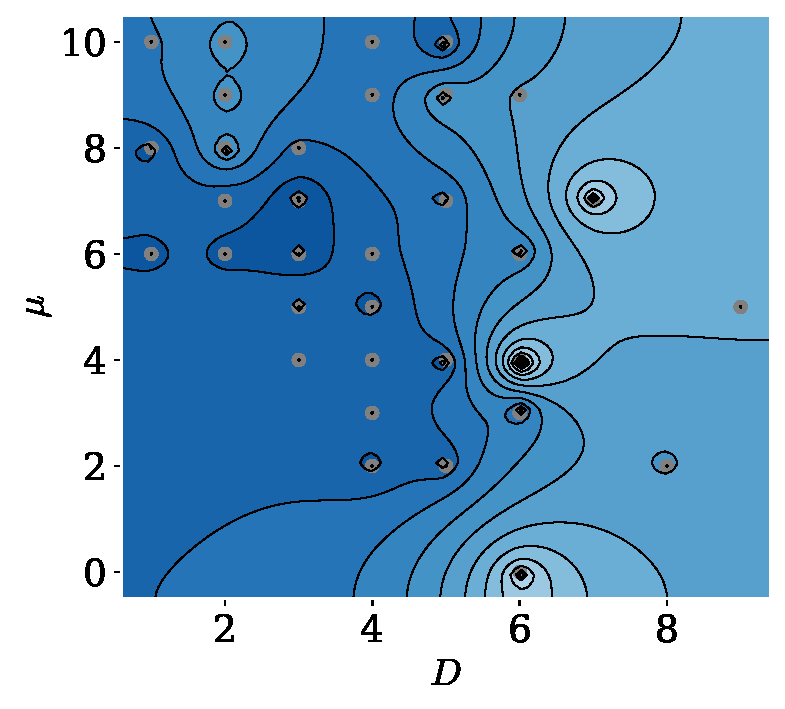
\includegraphics[width=\FW,height=\FH]{Figures/contour_D_vs_mu-14.pdf}} \\[0.6em]

% --------- FILA 2 ----------
\subfloat[$D'$ vs.$\mu$]{%
  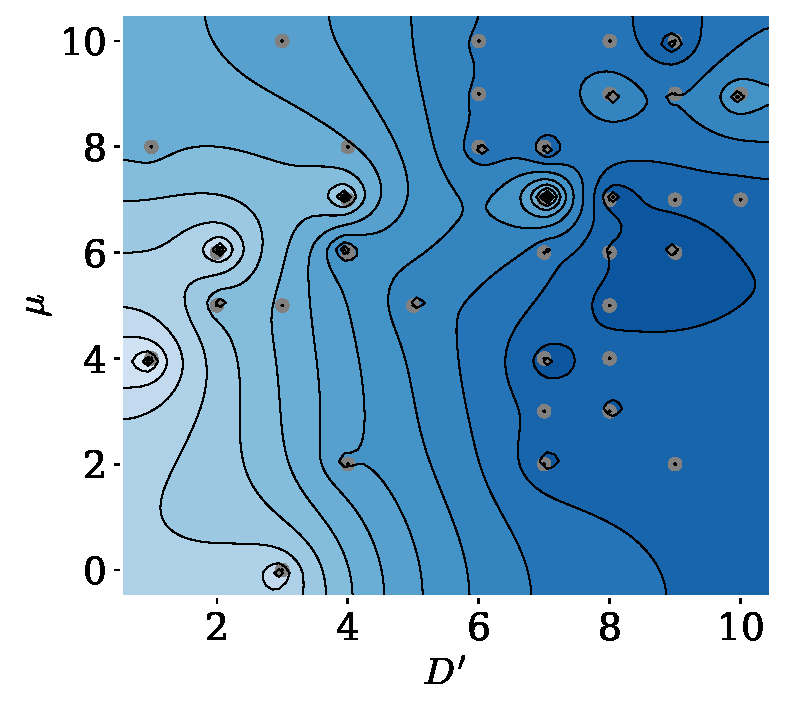
\includegraphics[width=\FW,height=\FH]{Figures/contour_Dprime_vs_mu-14.pdf}} 
\subfloat[$\tau$vs. $\mu$]{%
  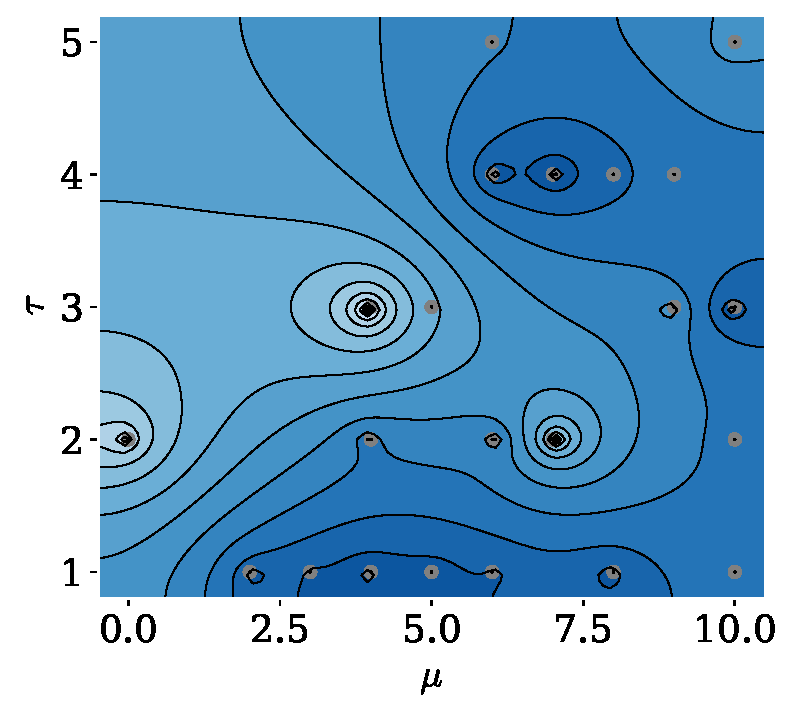
\includegraphics[width=\FW,height=\FH]{Figures/contour_mu_vs_tau-14.pdf}} 
\subfloat[$D'$ vs. $D$]{%
  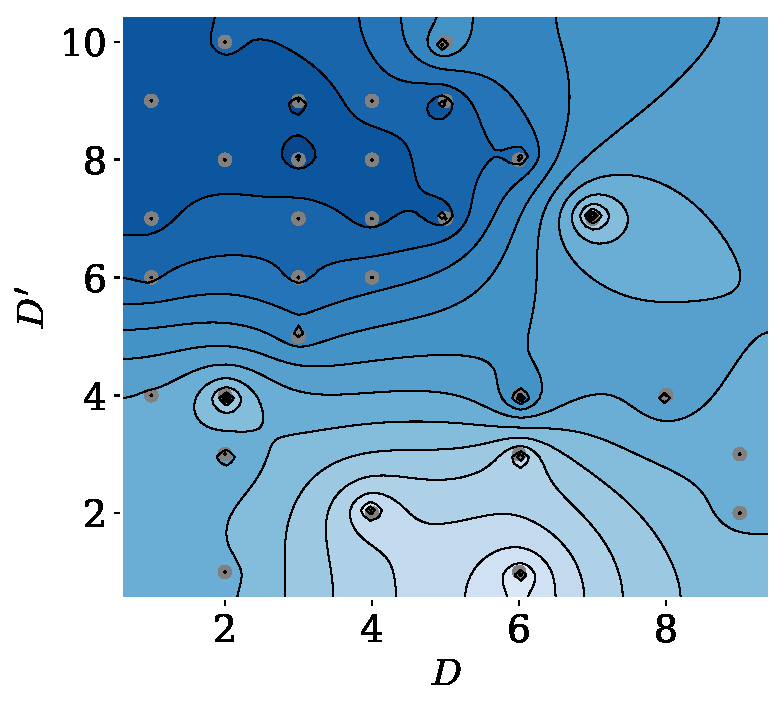
\includegraphics[width=\FW,height=\FH]{Figures/contour_D_vs_Dprime-14.pdf}} \\[0.8em]

% ================= COLORBAR HORIZONTAL (COMPARTIDO) =================
\begin{tikzpicture}
\begin{axis}[
  hide axis,
  scale only axis,
  width=\linewidth,
  height=0pt,
  colormap name=optunablues,
  colorbar horizontal,
  point meta min=60,
  point meta max=92,
  colorbar style={
    width=\linewidth,
    height=3mm,
    xtick={60, 64, 68, 72, 76, 80, 84, 88, 92},
    xticklabel style={font=\scriptsize},
    xlabel={val accuracy (\%)},
    xlabel style={font=\scriptsize, yshift=2pt},
    scaled ticks=false,
    /pgf/number format/fixed,
    /pgf/number format/precision=1,
  },
]
\addplot [draw=none] coordinates {(0,0)};
\end{axis}
\end{tikzpicture}

\end{minipage}%
}

\caption{{Contour plots of validation accuracy (\%) for \gls{tektenet} as a function of selected hyperparameter pairs for Subject~14 from the GigaScience dataset. All panels share the same color scale, allowing direct visual comparison across hyperparameter pairs within the subject.}}
\label{fig:global_freq_Giga14}
\end{figure}

%----------------------------------------------------

{In contrast, for the low-performing subject (Subject~27), the contour plots in Fig.~\ref{fig:global_freq_giga27} reveal a more constrained and fragmented optimization landscape. Compared with Subject~14, the high-performance regions are less extended and appear more localized across the explored hyperparameter space. The projections involving the temporal kernel size $K$ and the embedding dimensions ($D$, $D'$) show that favorable validation accuracy is mainly achieved within specific combinations of temporal receptive field and reconstructed state-space dimensionality, rather than across broad parameter ranges. This suggests a stronger sensitivity to the joint selection of $K$, $D$, and $D'$ for this subject.}

{A similar behavior is observed in the projections involving the delay parameter $\mu$, where favorable regions appear in localized zones depending on the values of $D$, $D'$, and $\tau$. This indicates that the estimation of delayed directed dependencies is more sensitive to the alignment among embedding order, stride, and interaction delay, which is consistent with the role of state-space reconstruction and transfer entropy in modeling nonlinear directed interactions~\cite{schreiber2000measuring,staniek2008symbolic}. The $D$--$D'$ projection also lacks a broad dominant region of high performance, showing instead several separated configurations with moderate-to-favorable accuracy. Overall, these patterns suggest that Subject~27 represents a more challenging optimization regime for \gls{tektenet}, in which decoding performance depends more critically on the precise balance among temporal filtering, state-space reconstruction, and delay-related parameters.}

%----------------------------------------------------
\begin{figure}[H]
\centering

% ---------- Tamaños ----------
\setlength{\FW}{0.34\linewidth}
\setlength{\FH}{3.4cm}

\makebox[\textwidth][c]{%

% ================= PANEL 3x2 + COLORBAR =================
\begin{minipage}[c]{0.99\textwidth}
\centering

% --------- FILA 1 ----------
\subfloat[$D$ vs. $K$]{%
  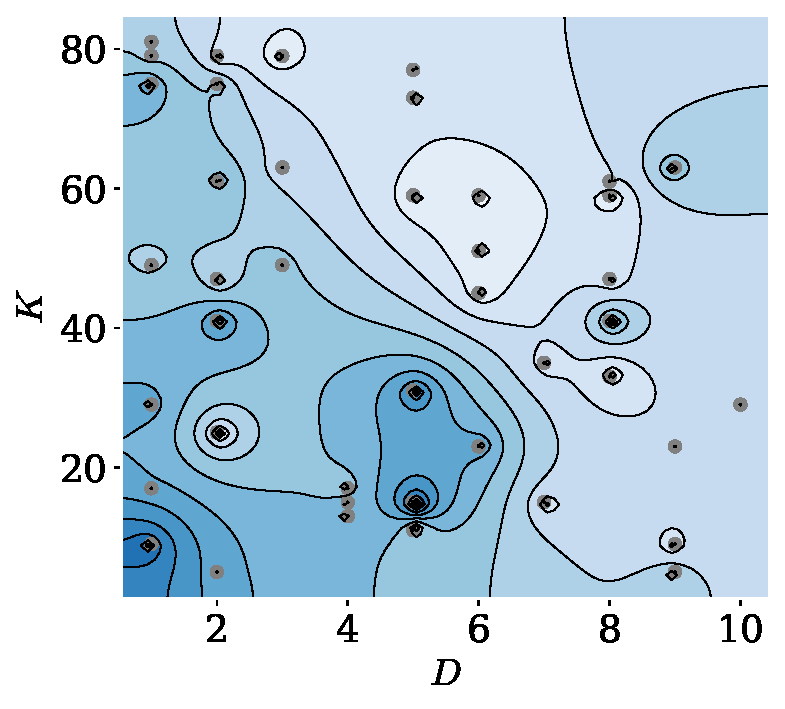
\includegraphics[width=\FW,height=\FH]{Figures/contour_D_vs_K-27.pdf}} 
\subfloat[$D'$ vs. $K$]{%
  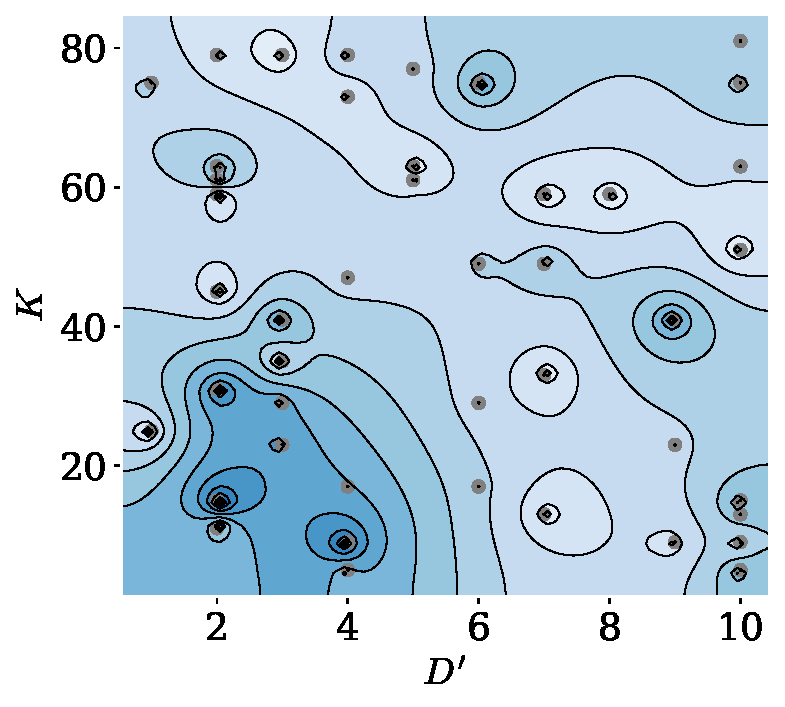
\includegraphics[width=\FW,height=\FH]{Figures/contour_Dprime_vs_K-27.pdf}} 
\subfloat[$D$ vs. $\mu$]{%
  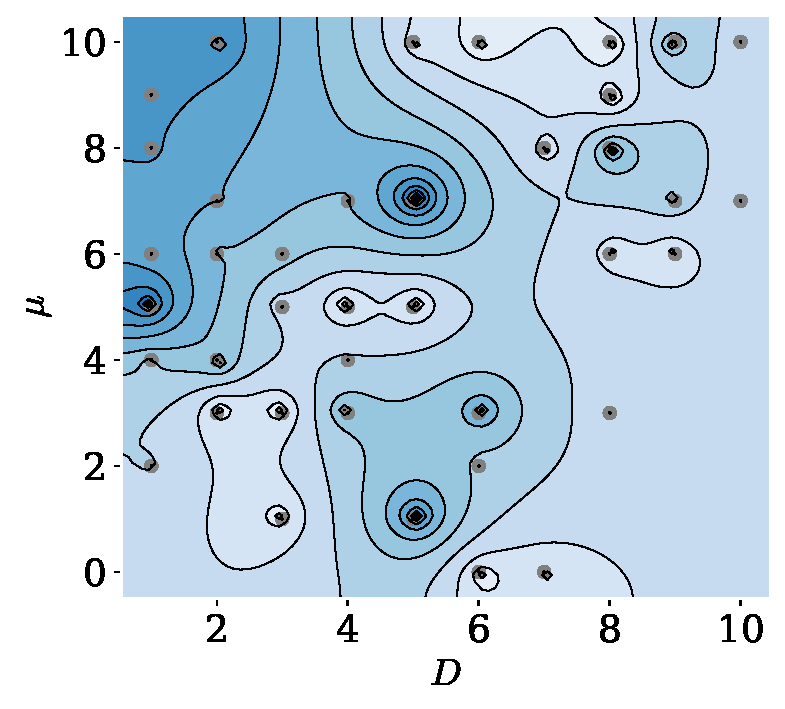
\includegraphics[width=\FW,height=\FH]{Figures/contour_D_vs_mu-27.pdf}} \\[0.6em]

% --------- FILA 2 ----------
\subfloat[$D'$ vs.$\mu$]{%
  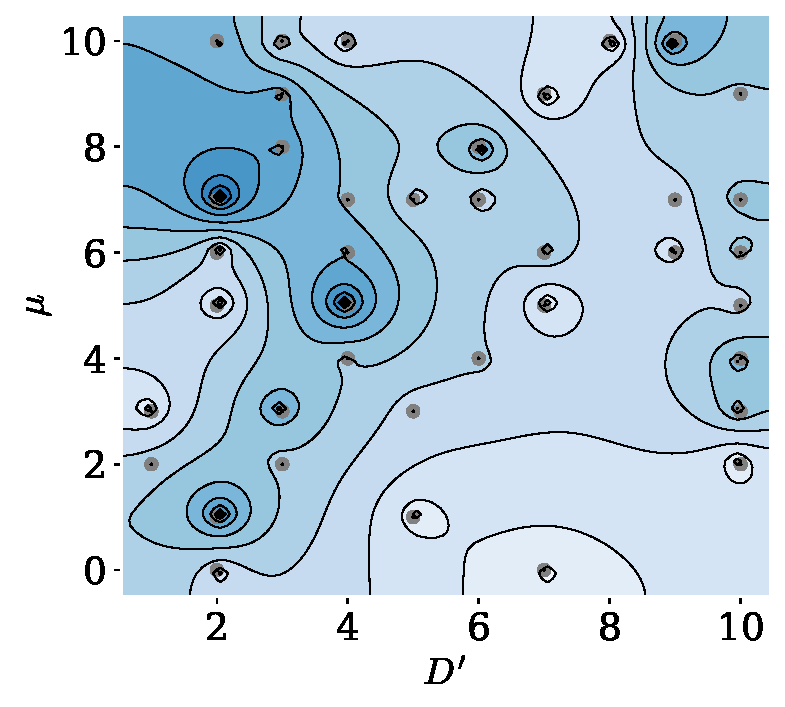
\includegraphics[width=\FW,height=\FH]{Figures/contour_Dprime_vs_mu-27.pdf}}
\subfloat[$\tau$vs. $\mu$]{%
  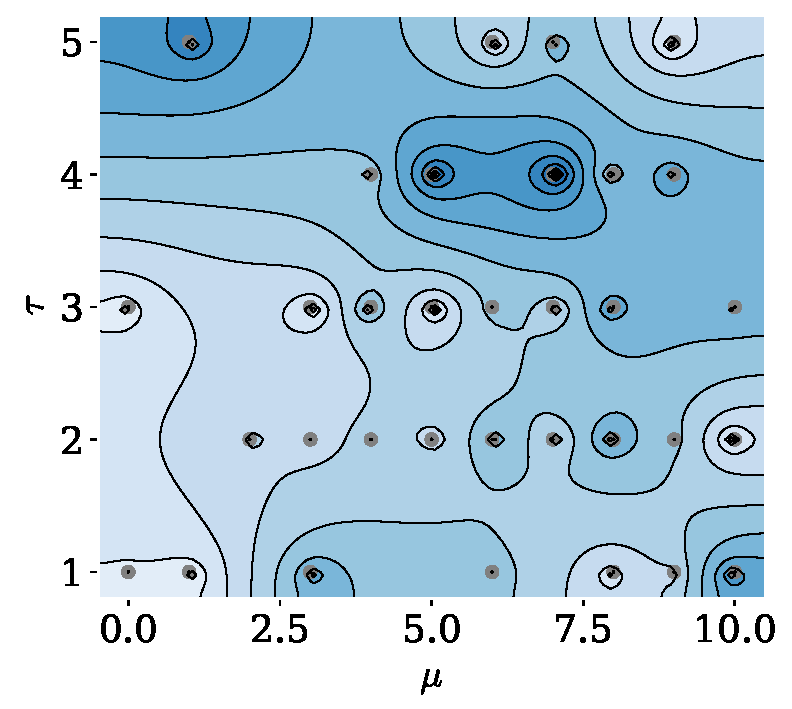
\includegraphics[width=\FW,height=\FH]{Figures/contour_mu_vs_tau-27.pdf}} 
\subfloat[$D'$ vs. $D$]{%
  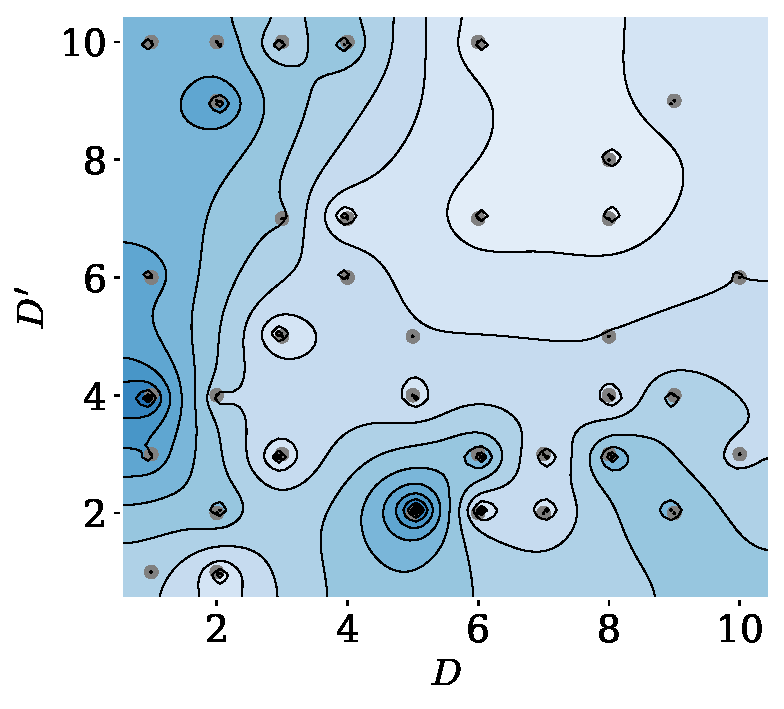
\includegraphics[width=\FW,height=\FH]{Figures/contour_D_vs_Dprime-27.pdf}} \\[0.8em]

% ================= COLORBAR HORIZONTAL (COMPARTIDO) =================
\begin{tikzpicture}
\begin{axis}[
  hide axis,
  scale only axis,
  width=\linewidth,
  height=0pt,
  colormap name=optunablues,
  colorbar horizontal,
  point meta min=51,
  point meta max=65,
  colorbar style={
    width=\linewidth,
    height=3mm,
    xtick={51, 53, 55, 57, 59, 61, 63, 65},
    xticklabel style={font=\scriptsize},
    xlabel={val accuracy (\%)},
    xlabel style={font=\scriptsize, yshift=2pt},
    scaled ticks=false,
    /pgf/number format/fixed,
    /pgf/number format/precision=1,
  },
]
\addplot [draw=none] coordinates {(0,0)};
\end{axis}
\end{tikzpicture}

\end{minipage}%
}

\caption{{Contour plots of validation accuracy (\%) for \gls{tektenet} as a function of selected hyperparameter pairs for Subject~27 from the GigaScience dataset. All panels share the same color scale, allowing direct visual comparison across hyperparameter pairs within the subject.}}
\label{fig:global_freq_giga27}
\end{figure}
%----------------------------------------------------
{To complement the subject-specific contour analysis, a global hyperparameter-importance analysis was conducted to quantify the relative contribution of each \gls{tektenet} hyperparameter to validation accuracy on the GigaScience dataset. As shown in Fig.~\ref{fig:GIGA_TE}, this analysis summarizes the influence of the temporal kernel size $K$, the stride $\tau$, the embedding orders $D$ and $D'$, and the interaction delay $\mu$ across the explored hyperparameter configurations.}

{The results show that the temporal kernel size $K$ and the stride $\tau$ are the most influential hyperparameters, with importance scores of $0.33$ and $0.31$, respectively. Together, these two parameters account for the largest proportion of the global importance, suggesting that \gls{tektenet} performance on the GigaScience dataset is mainly driven by the temporal receptive field and the stride-related sampling of the reconstructed dynamics. This result highlights the relevance of how temporal information is locally filtered and subsequently organized for Takens-based connectivity estimation~\cite{schreiber2000measuring}.}

{In contrast, the embedding order $D$ and the interaction delay $\mu$ exhibit moderate importance scores of $0.15$ and $0.14$, respectively, indicating that state-space reconstruction and delayed directed interactions also contribute to validation accuracy, although their influence is secondary compared with $K$ and $\tau$. Finally, $D'$ shows the lowest importance score ($0.07$), suggesting that, within the explored range, \gls{tektenet} is less sensitive to this embedding dimension. Overall, these findings indicate that temporal filtering and stride-related dynamics constitute the main drivers of performance, while the remaining Takens-based parameters provide complementary adjustments to the effective-connectivity representation.}
%----------------------------------------------------
\begin{figure}[H]
    \centering
    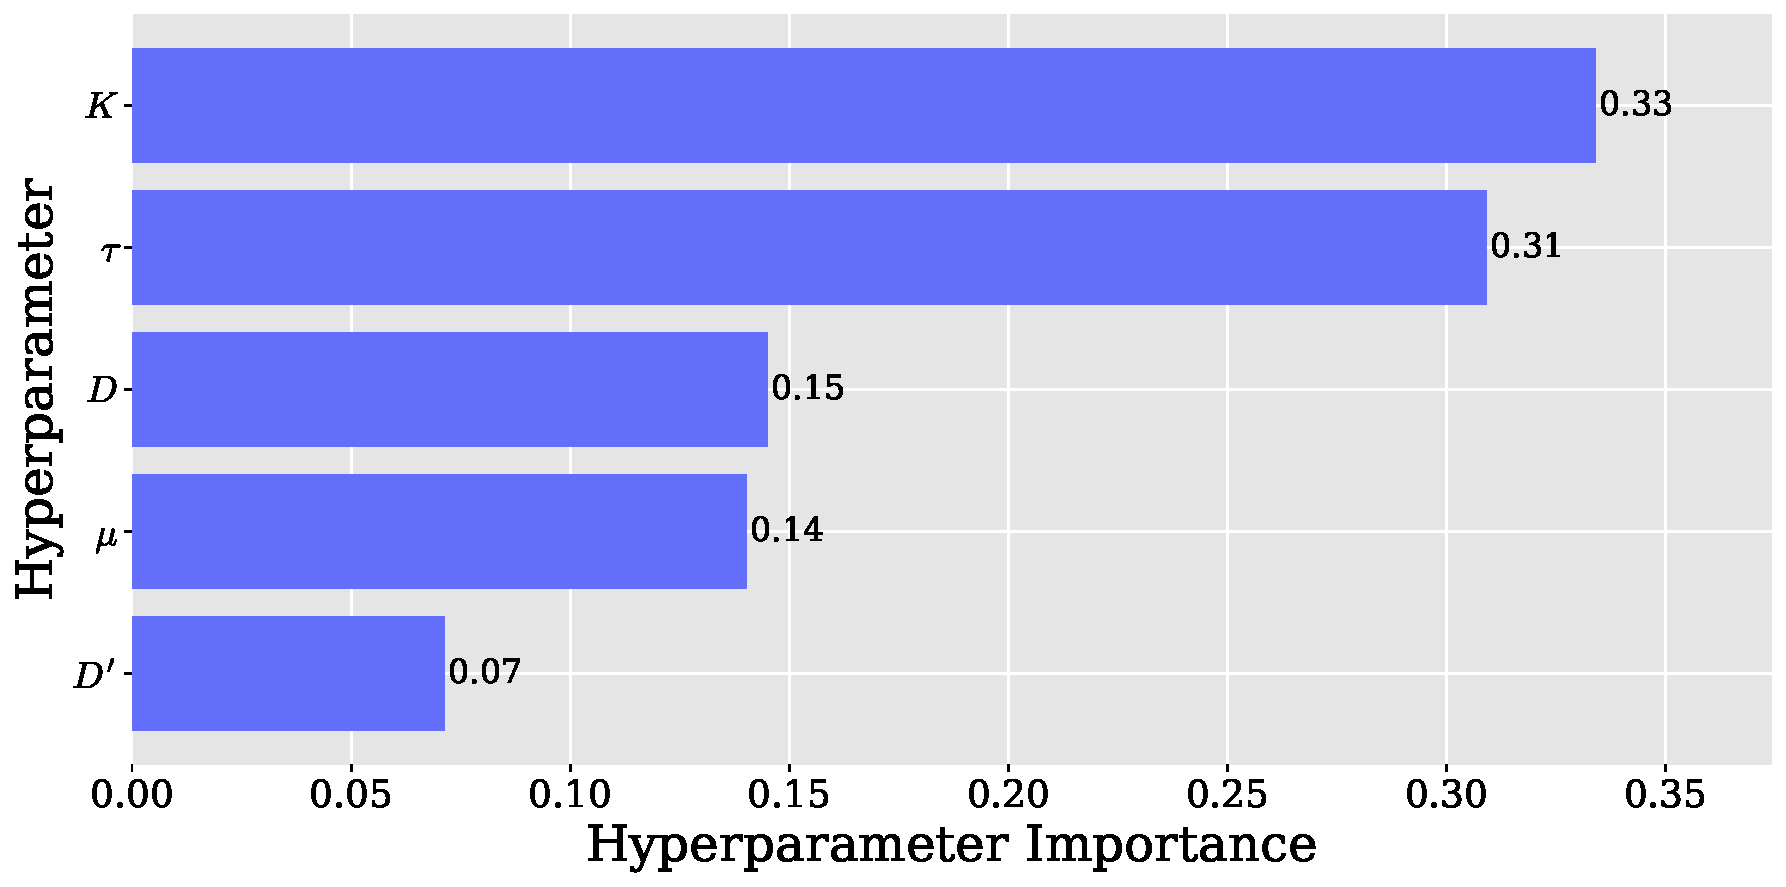
\includegraphics[width=0.8\linewidth]{Figures/optuna_fanova_param_importances_tekte-GIGA.pdf}
    \caption{{Global hyperparameter importance analysis for \gls{tektenet} on the GigaScience dataset. Importance scores quantify the relative contribution of the temporal kernel size $K$, stride $\tau$, embedding orders $D$ and $D'$, and interaction delay $\mu$ to validation accuracy.}}
    \label{fig:GIGA_TE}
\end{figure}
%----------------------------------------------------


\subsubsection{Validation on complex scenarios: Multi-class decoding on \gls{eegmmidb} collection}

To assess the scalability of the proposed framework beyond binary classification, its performance was evaluated on the \gls{eegmmidb} dataset, which poses a challenging five-class \gls{mi} decoding task. This scenario requires the model to disentangle multiple distinct neural patterns (Left Hand, Right Hand, Both Hands, Both Feet, and Rest), thereby significantly increasing the complexity of the decision boundaries compared to the binary BCI Competition IV-2a setting {evaluated within this contribution}.

Beyond the overall classification results, this experiment also enabled an analysis of the robustness and adaptability of the proposed framework under inter-subject variability by incorporating a systematic Bayesian hyperparameter optimization procedure. For each subject, the model's structural and temporal hyperparameters, namely the embedding orders $D$ and $D'$, the stride $\tau$, the interaction delay $\mu$, and the temporal kernel size $K$, were automatically tuned to maximize validation performance under a controlled evaluation protocol.

%---------------------------------------------------------------------------------
\begin{table}[htbp]
\centering
\caption{Subject-specific \gls{tektenet} hyperparameters selected through Bayesian optimization on the \gls{eegmmidb} dataset.}
\label{tab:hyperparameters_physionet}
\begin{tabular}{crrrrrr}
\toprule
\textbf{Subject} & \textbf{$D$} & \textbf{$D'$} & \textbf{$\tau$} & \textbf{$\mu$} & \textbf{$K$} & \textbf{Val. Acc. (\%)} \\
\midrule
3   & 3 & 1 & 3 & 16 & 16 & 76.19 \\
7   & 4 & 4 & 3 & 16 & 22 & 74.61 \\
8   & 1 & 1 & 4 & 13 & 32 & 77.78 \\
9   & 3 & 3 & 3 & 11 & 22 & 74.60 \\
12  & 4 & 4 & 4 & 12 & 16 & 77.77 \\
13  & 6 & 3 & 2 & 19 & 22 & 77.76 \\
40  & 5 & 1 & 5 & 18 & 22 & 74.59 \\
41  & 6 & 3 & 4 & 10 & 22 & 76.18 \\
49  & 1 & 4 & 4 & 17 & 16 & 77.75 \\
50  & 1 & 1 & 4 & 10 & 16 & 77.74 \\
\midrule
\textbf{Average} &  &  &  &  &  & \textbf{76.50} \\
\bottomrule
\end{tabular}
\end{table}
%---------------------------------------------------------------------------------
The results summarized in Table~\ref{tab:hyperparameters_physionet} show that \gls{tektenet} achieves stable validation performance across the evaluated subjects, with an average validation accuracy of $76.50\%$ in the five-class \gls{eegmmidb} scenario. Despite the increased complexity of multi-class decoding, the subject-wise validation accuracies remain within a relatively narrow range, from $74.59\%$ to $77.78\%$. This suggests that the Bayesian optimization procedure was able to identify subject-specific hyperparameter configurations that preserve consistent performance under heterogeneous \gls{eeg} conditions~\cite{snoek2012practical}.

The selected configurations also show variability across subjects, particularly in the embedding orders $D$ and $D'$, the interaction delay $\mu$, and the temporal kernel size $K$. This behavior indicates that different subjects may require different balances between state-space reconstruction, temporal filtering, and delayed directed-dependency modeling, which is consistent with the role of embedding-based reconstruction and transfer entropy in capturing nonlinear directed interactions~\cite{takens1981detecting,schreiber2000measuring}. Therefore, the results support the relevance of subject-adaptive hyperparameter tuning when scaling \gls{tektenet} from binary decoding scenarios to more complex multi-class \gls{mi} tasks.

Overall, these findings suggest that the joint integration of connectivity-driven representations and Bayesian hyperparameter optimization contributes to the scalability of \gls{tektenet} on the \gls{eegmmidb} dataset, allowing the proposed framework to adapt its temporal and embedding-related parameters while preserving stable inter-subject validation performance.

%--------------------------------------------------------
%% Contours 
%--------------------------------------------------------
{To further characterize the hyperparameter landscape in this multi-class scenario, contour plots were generated for two representative subjects from the \gls{eegmmidb} dataset: Subject~12 and Subject~41. These subjects were selected to maintain consistency with the previous EEG-GCIRNet analysis, where Subject~12 represented a high-performing case and Subject~41 corresponded to a comparatively more challenging subject in the same multi-class setting. Using the same subjects allows a coherent cross-method interpretation of how different connectivity-aware frameworks behave under favorable and difficult subject-specific conditions.}

{The plots show how validation accuracy varies across selected pairs of \gls{tektenet} hyperparameters based on the configurations evaluated during the Bayesian optimization process. Thus, the contour analysis provides a visual approximation of the explored hyperparameter performance landscape, allowing the identification of favorable regions, localized optima, and configurations in which the model becomes more sensitive to specific hyperparameter choices.}
%----------------------------------------------------------
%---------------------------------------------------------------------------------
\begin{figure}[H]
\centering

% ---------- Tamaños ----------
\setlength{\FW}{0.34\linewidth}
\setlength{\FH}{3.4cm}

\makebox[\textwidth][c]{%

% ================= PANEL 3x2 + COLORBAR =================
\begin{minipage}[c]{0.99\textwidth}
\centering

% --------- FILA 1 ----------
\subfloat[$D$ vs. $K$]{%
  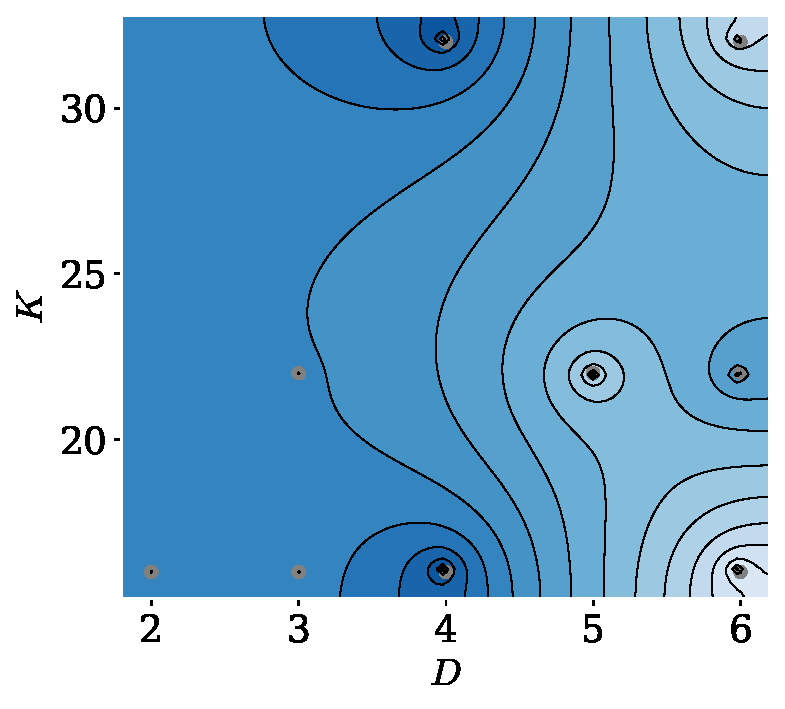
\includegraphics[width=\FW,height=\FH]{Figures/contour_D_vs_K-12.pdf}} 
\subfloat[$D'$ vs. $K$]{%
  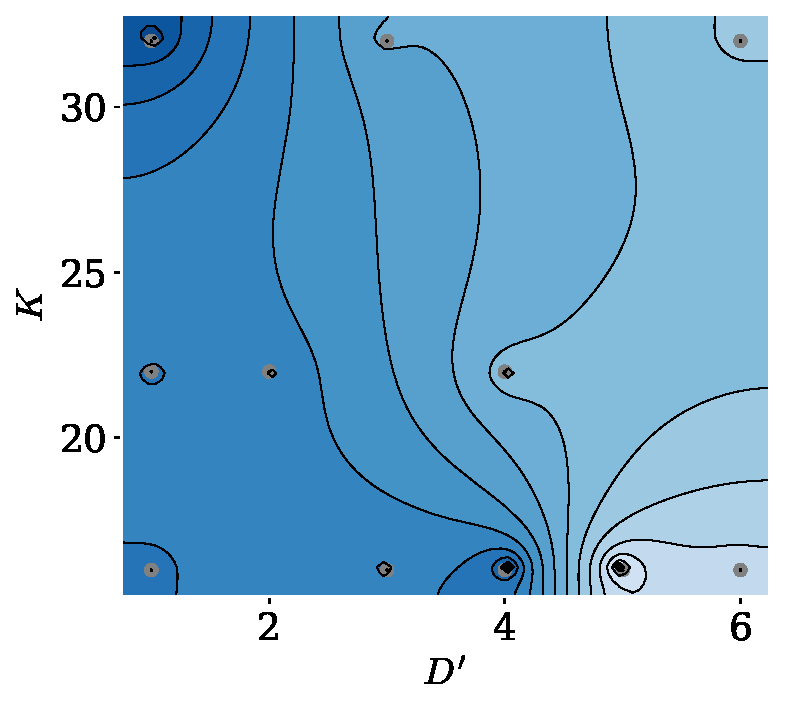
\includegraphics[width=\FW,height=\FH]{Figures/contour_Dprime_vs_K-12.pdf}} 
\subfloat[$D$vs. $\mu$]{%
  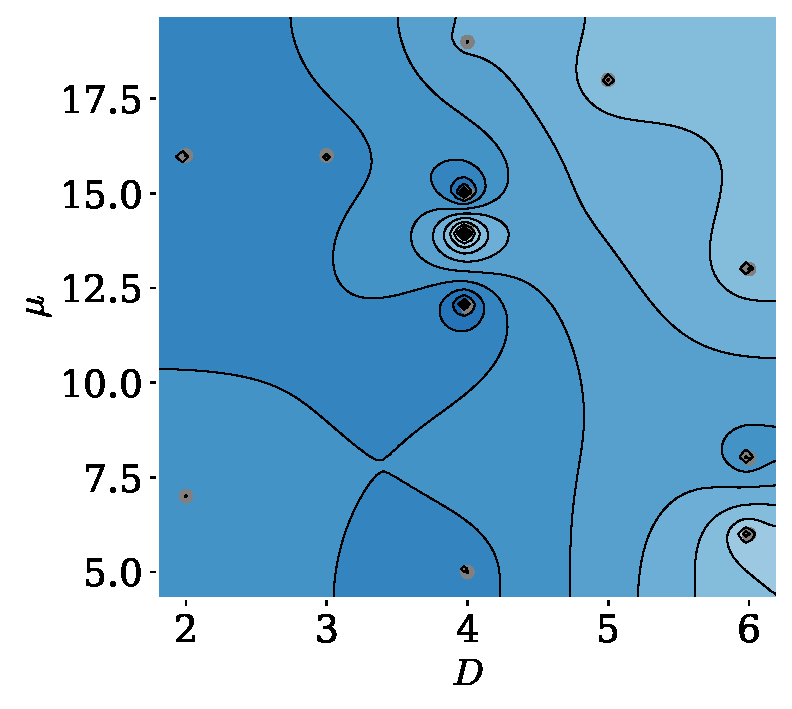
\includegraphics[width=\FW,height=\FH]{Figures/contour_D_vs_mu-12.pdf}} \\[0.6em]

% --------- FILA 2 ----------
\subfloat[$D'$ vs.$\mu$]{%
  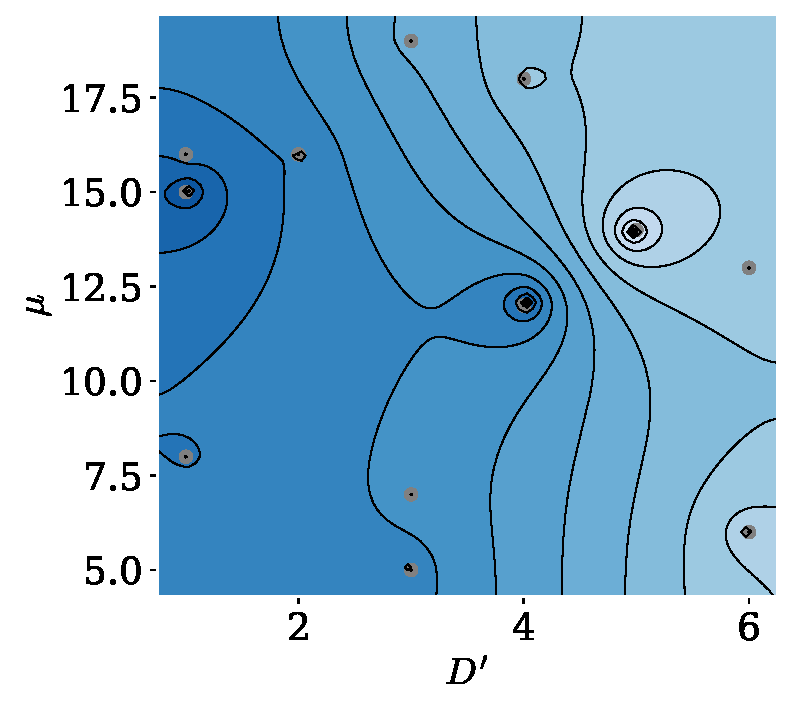
\includegraphics[width=\FW,height=\FH]{Figures/contour_Dprime_vs_mu-12.pdf}} 
\subfloat[$\tau$vs. $\mu$]{%
  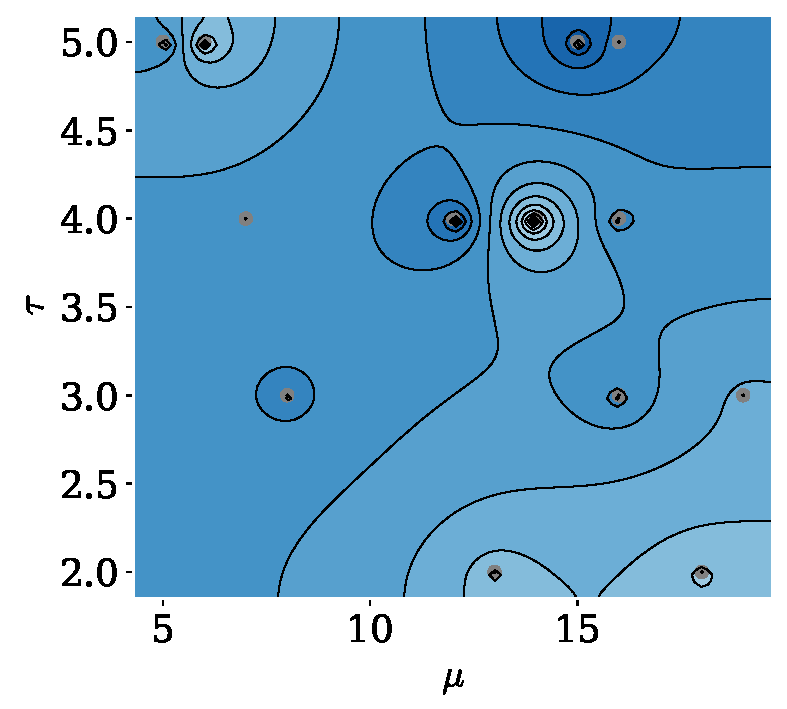
\includegraphics[width=\FW,height=\FH]{Figures/contour_mu_vs_tau-12.pdf}}
\subfloat[$D'$ vs. $D$]{%
  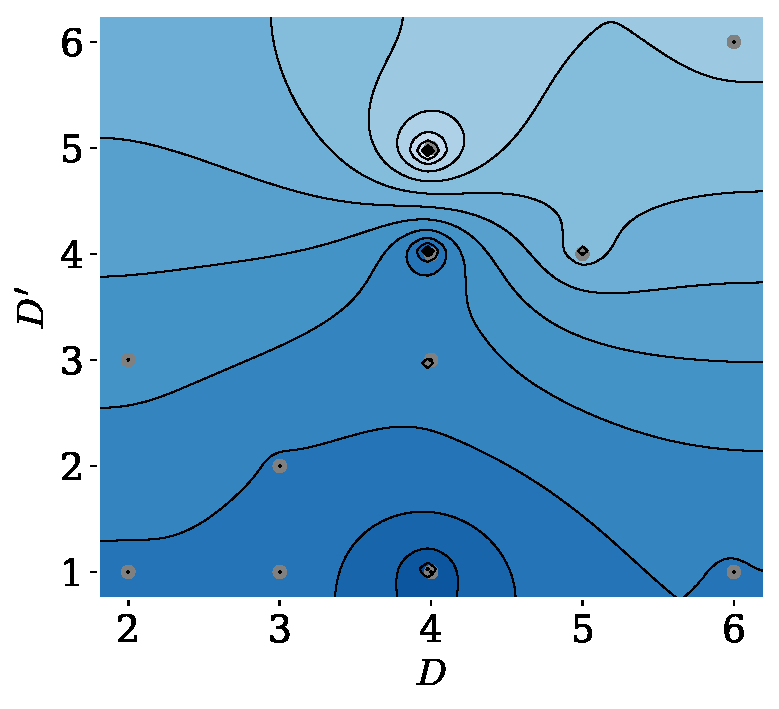
\includegraphics[width=\FW,height=\FH]{Figures/contour_D_vs_Dprime-12.pdf}} \\[0.8em]

% ================= COLORBAR HORIZONTAL (COMPARTIDO) =================
\begin{tikzpicture}
\begin{axis}[
  hide axis,
  scale only axis,
  width=\linewidth,
  height=0pt,
  colormap name=optunablues,
  colorbar horizontal,
  point meta min=64.8,
  point meta max=77.6,
  colorbar style={
    width=\linewidth,
    height=3mm,
    xtick={64.8,66.4,68.0,69.6,71.2,72.8,74.4,76.0,77.6},
    xticklabel style={font=\scriptsize},
    xlabel={val accuracy (\%)},
    xlabel style={font=\scriptsize, yshift=2pt},
    scaled ticks=false,
    /pgf/number format/fixed,
    /pgf/number format/precision=1,
  },
]
\addplot [draw=none] coordinates {(0,0)};
\end{axis}
\end{tikzpicture}

\end{minipage}%
}

\caption{{Contour plots of validation accuracy (\%) for \gls{tektenet} as a function of selected hyperparameter pairs for Subject~12 from the \gls{eegmmidb} dataset. All panels share the same color scale, allowing direct visual comparison across hyperparameter pairs within the subject.}}
\label{fig:global_freq_Phy12}
\end{figure}

%---------------------------------------------------------------------------------
{For the high-performing subject (Subject~12), the contour plots in Fig.~\ref{fig:global_freq_Phy12} reveal a relatively organized and structured optimization landscape, with well-defined high-performance regions rather than highly fragmented optima. In particular, the projections involving the temporal kernel size $K$ suggest that better validation accuracy is generally associated with larger receptive fields combined with low-to-moderate embedding orders. Likewise, the $\mu$-based projections show organized and interpretable trends, with favorable regions concentrated around intermediate values of $\mu$ and only localized performance drops for specific hyperparameter combinations. The $\mu$--$\tau$ interaction also remains relatively coherent, indicating that the alignment between interaction delay and stride is reasonably stable for this subject, which is consistent with the role of temporal embedding choices in nonlinear directed-dependency estimation~\cite{takens1981detecting, schreiber2000measuring}. Finally, the $D$--$D'$ interaction exhibits a structured surface with several competitive configurations, although jointly large embedding orders appear less favorable. Overall, these patterns suggest that, even in this more challenging multi-class setting, \gls{tektenet} operates under a relatively favorable hyperparameter regime for high-performing subjects, where performance depends on structured parameter interactions rather than on isolated sharp optima.}

%---------------------------------------------------------------------------------
\begin{figure}[H]
\centering

% ---------- Tamaños ----------
\setlength{\FW}{0.34\linewidth}
\setlength{\FH}{3.4cm}

\makebox[\textwidth][c]{%

% ================= PANEL 3x2 + COLORBAR =================
\begin{minipage}[c]{0.99\textwidth}
\centering

% --------- FILA 1 ----------
\subfloat[$D$ vs. $K$]{%
  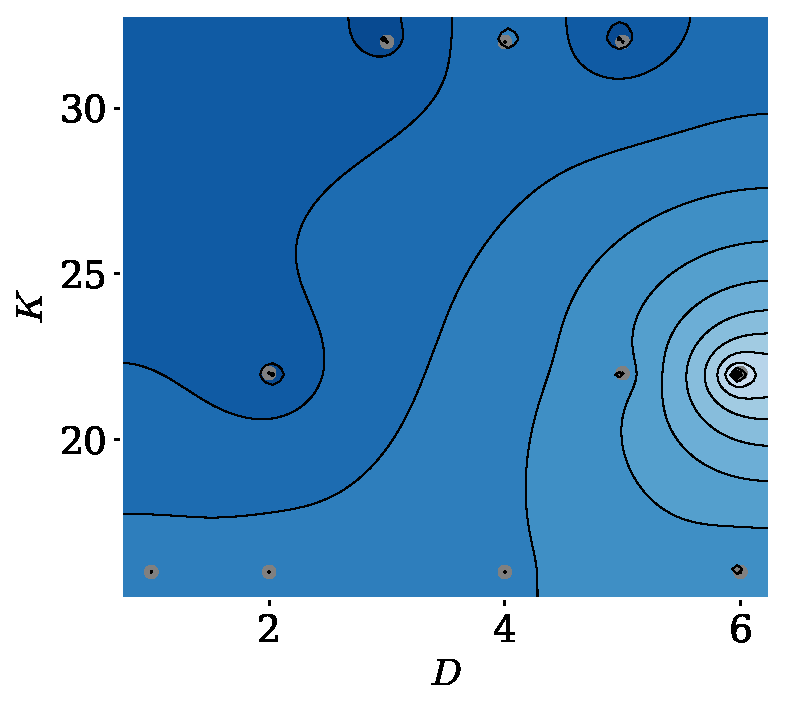
\includegraphics[width=\FW,height=\FH]{Figures/contour_D_vs_K-41.pdf}} 
\subfloat[$D'$ vs. $K$]{%
  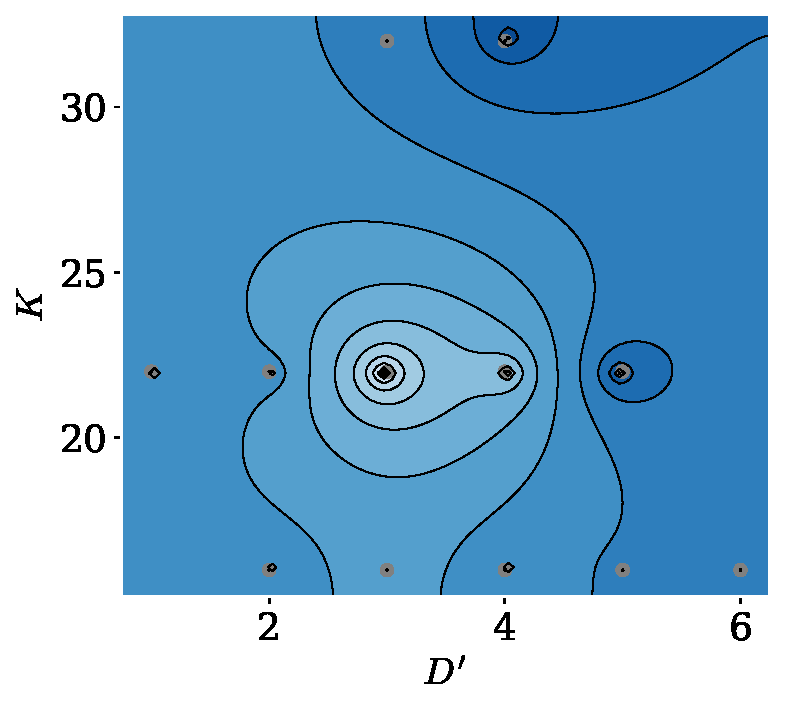
\includegraphics[width=\FW,height=\FH]{Figures/contour_Dprime_vs_K-41.pdf}} 
\subfloat[$D$vs. $\mu$]{%
  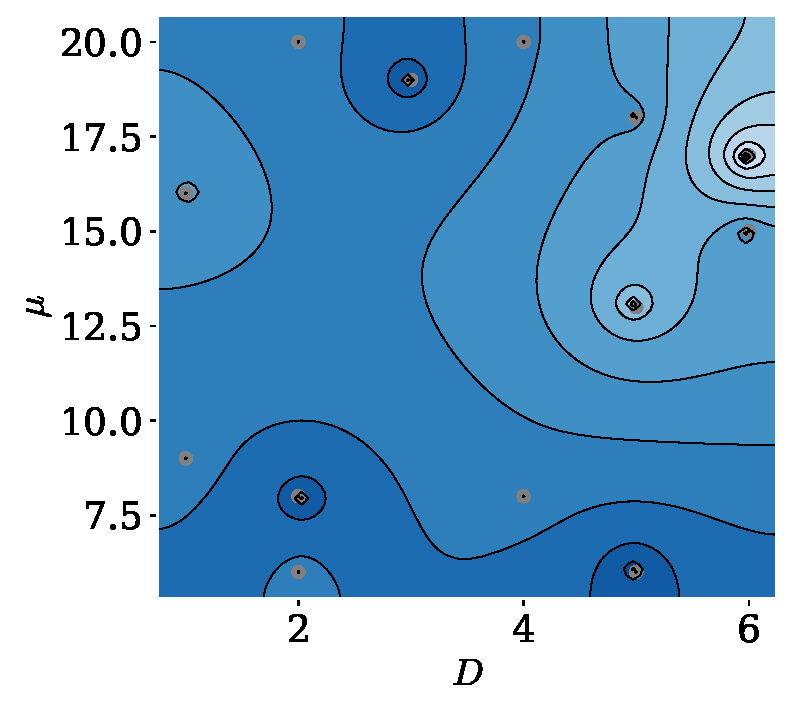
\includegraphics[width=\FW,height=\FH]{Figures/contour_D_vs_mu-41.pdf}} \\[0.6em]

% --------- FILA 2 ----------
\subfloat[$D'$ vs.$\mu$]{%
  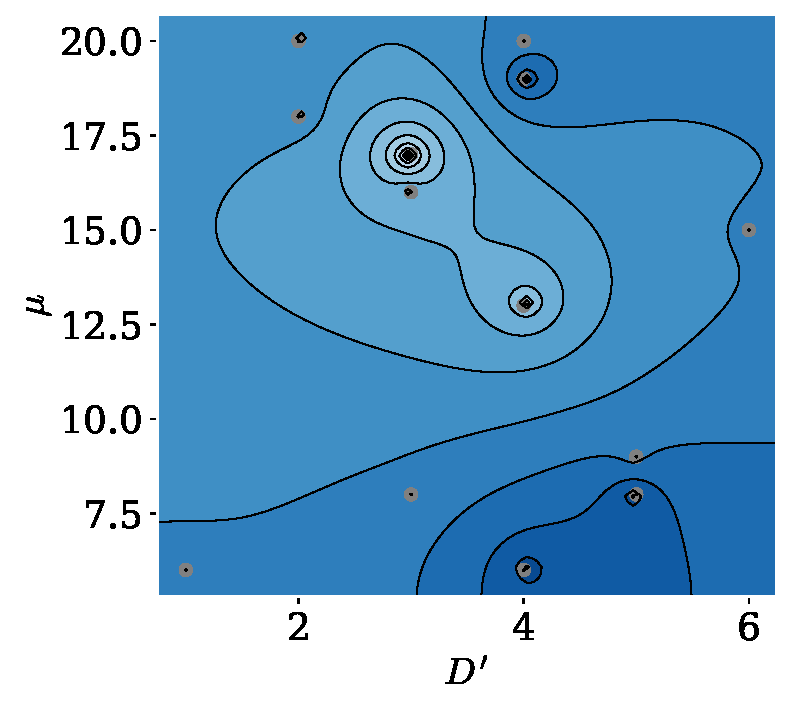
\includegraphics[width=\FW,height=\FH]{Figures/contour_Dprime_vs_mu-41.pdf}}
\subfloat[$\tau$vs. $\mu$]{%
  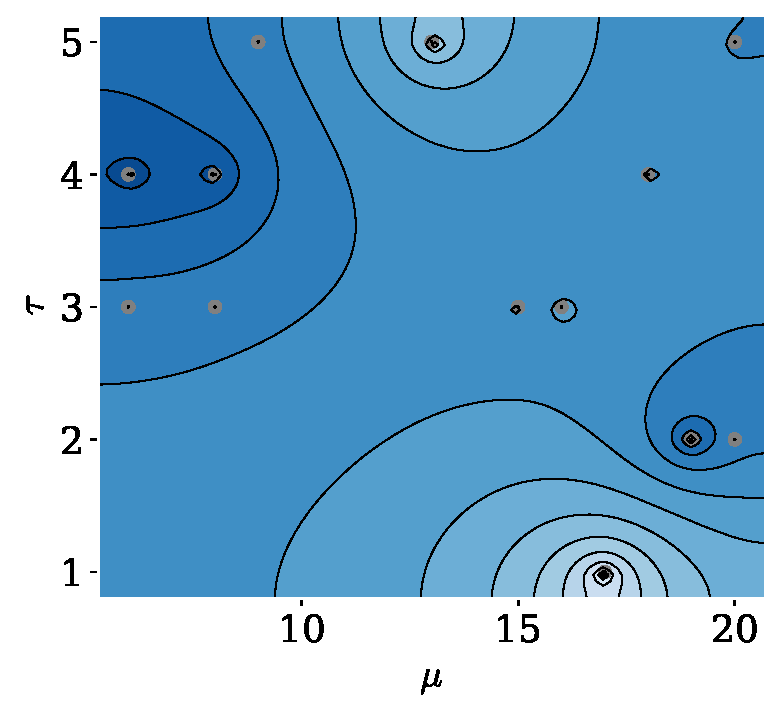
\includegraphics[width=\FW,height=\FH]{Figures/contour_mu_vs_tau-41.pdf}} 
\subfloat[$D'$ vs. $D$]{%
  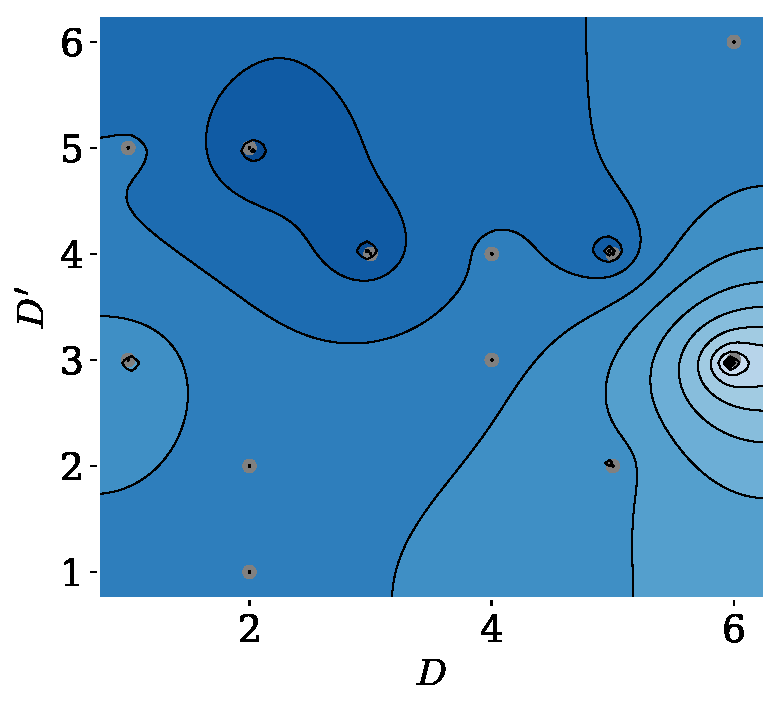
\includegraphics[width=\FW,height=\FH]{Figures/contour_D_vs_Dprime-41.pdf}} \\[0.8em]

% ================= COLORBAR HORIZONTAL (COMPARTIDO) =================
\begin{tikzpicture}
\begin{axis}[
  hide axis,
  scale only axis,
  width=\linewidth,
  height=0pt,
  colormap name=optunablues,
  colorbar horizontal,
  point meta min=64.8,
  point meta max=76.2,
  colorbar style={
    width=\linewidth,
    height=3mm,
    xtick={64.8,66.4,68.0,69.6,71.2,72.8,74.4,76.2},
    xticklabel style={font=\scriptsize},
    xlabel={val accuracy (\%)},
    xlabel style={font=\scriptsize, yshift=2pt},
    scaled ticks=false,
    /pgf/number format/fixed,
    /pgf/number format/precision=1,
  },
]
\addplot [draw=none] coordinates {(0,0)};
\end{axis}
\end{tikzpicture}

\end{minipage}%
}

\caption{{Contour plots of validation accuracy (\%) for \gls{tektenet} as a function of selected hyperparameter pairs for Subject~41 from the \gls{eegmmidb} dataset. The shared color scale enables direct comparison across hyperparameter interactions within this subject.}}
\label{fig:global_freq_Phy41}
\end{figure}
%----------------------------------------------------
{In contrast, for Subject~41, the contour plots in Fig.~\ref{fig:global_freq_Phy41} reveal a less homogeneous and more subject-sensitive optimization landscape, with favorable regions interrupted by localized performance drops. In the projections involving the temporal kernel size $K$, performance appears more sensitive to its interaction with the embedding orders, particularly around intermediate regions where narrower low-performance valleys emerge. A similar behavior is observed in the $\mu$-based projections, which show stronger fluctuations and less uniformly structured favorable regions than those observed for Subject~12.}

{The $\mu$--$\tau$ interaction is especially indicative of this behavior, with more pronounced transitions between favorable and less favorable zones. This suggests that the alignment between interaction delay and stride must be more carefully adjusted for this subject, which is consistent with the role of temporal embedding choices in nonlinear directed-dependency estimation~\cite{takens1981detecting, schreiber2000measuring}. The $D$--$D'$ interaction also lacks a single broad dominant regime, instead exhibiting multiple localized configurations with comparable performance. Overall, these patterns suggest that, in this multi-class setting, \gls{tektenet} operates under a sharper and more subject-sensitive hyperparameter regime for comparatively more challenging subjects, where performance depends more critically on the coordination among temporal filtering, state-space reconstruction, and delay-related parameters.}

{To complement the subject-specific contour analysis, a global hyperparameter-importance analysis was conducted to quantify the relative contribution of each \gls{tektenet} hyperparameter to validation accuracy on the \gls{eegmmidb} dataset. As shown in Fig.~\ref{fig:PHYSIONET_TE}, this analysis summarizes the influence of the embedding orders $D$ and $D'$, the interaction delay $\mu$, the stride $\tau$, and the temporal kernel size $K$ across the explored hyperparameter configurations.}

{The results show that the embedding orders $D'$ and $D$ are the most influential hyperparameters, with importance scores of $0.40$ and $0.27$, respectively. Together, these parameters account for the largest proportion of the global importance, suggesting that \gls{tektenet} performance on the \gls{eegmmidb} dataset is mainly driven by the configuration of the reconstructed state-space representation. This result indicates that, in the five-class decoding scenario, the ability to organize temporal information through suitable embedding orders plays a central role in separating multiple motor-imagery-related neural patterns.}

{The interaction delay $\mu$ also exhibits a relevant contribution, with an importance score of $0.19$, indicating that delayed directed dependencies remain important for modeling nonlinear temporal interactions across \gls{eeg} channels. This behavior is consistent with the role of state-space reconstruction and transfer entropy in capturing nonlinear directed interactions between time series~\cite{takens1981detecting, schreiber2000measuring}. In contrast, the stride $\tau$ and the temporal kernel size $K$ show lower importance scores of $0.09$ and $0.05$, respectively, suggesting that, within the explored range, \gls{tektenet} is less sensitive to temporal sampling and local temporal filtering than to the embedding-related parameters. Overall, these findings indicate that \gls{tektenet} performance on the \gls{eegmmidb} dataset is primarily governed by the structure of the reconstructed embedding space, while delay-related and temporal-filtering parameters provide complementary adjustments to the effective-connectivity representation.}

%----------------------------------------------------
\begin{figure}[H]
    \centering
    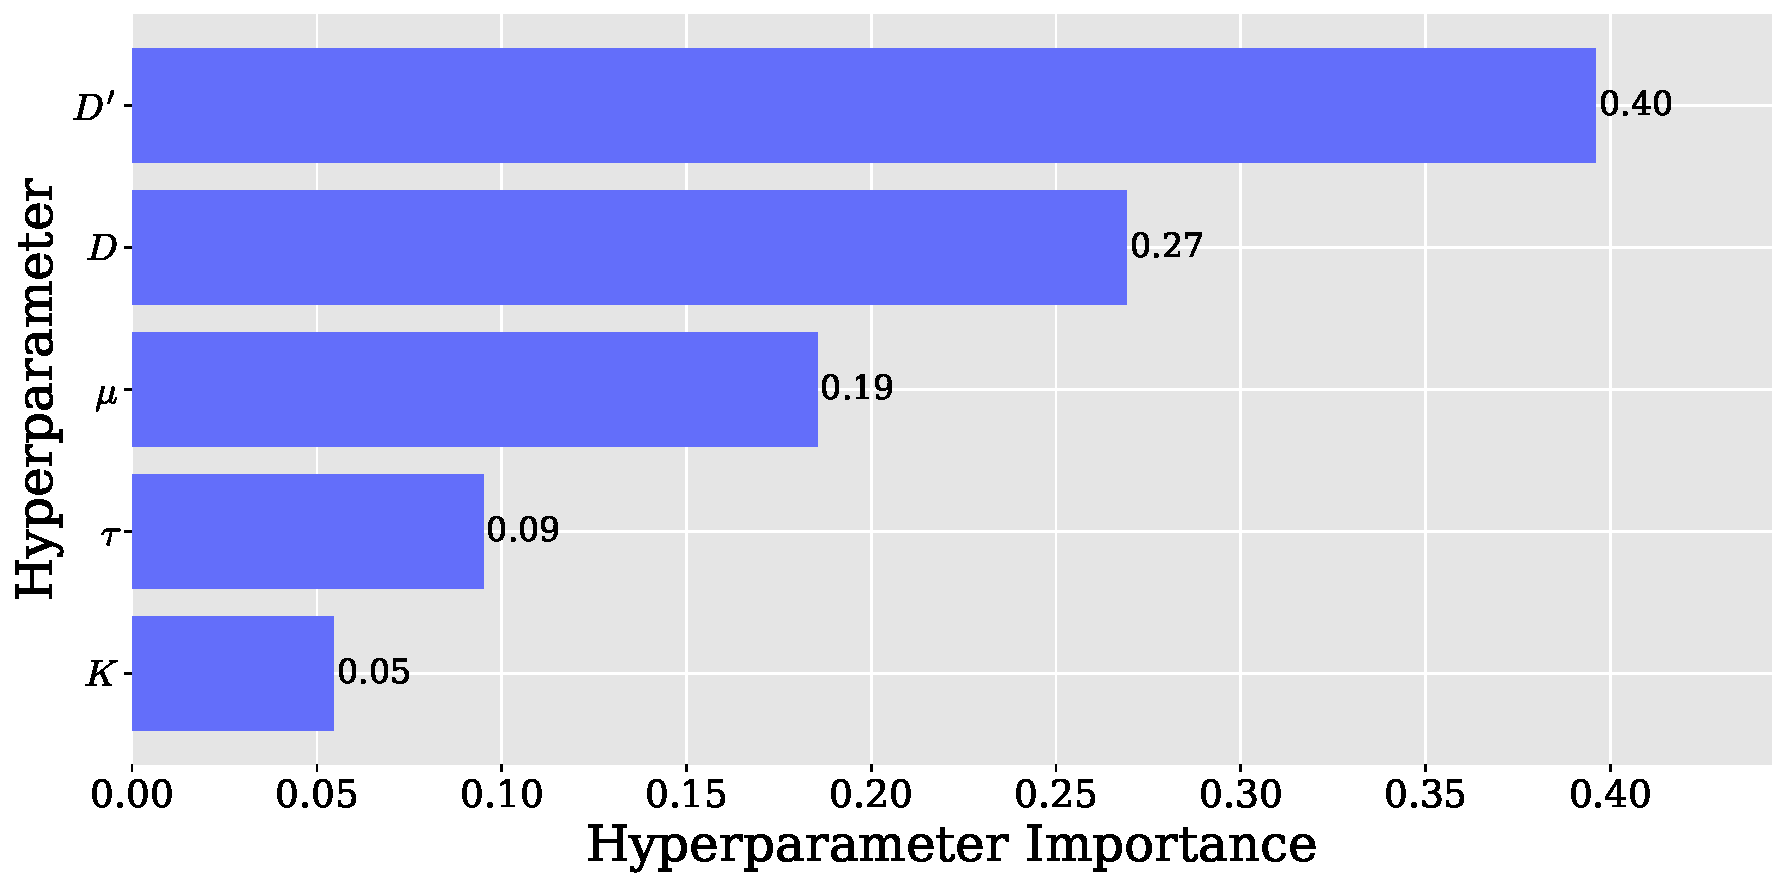
\includegraphics[width=0.8\linewidth]{Figures/optuna_fanova_param_importances_tekte-PHYSIONET.pdf}
    \caption{{Global hyperparameter importance analysis for \gls{tektenet} on the \gls{eegmmidb} dataset. Importance scores quantify the relative contribution of the embedding orders $D$ and $D'$, interaction delay $\mu$, stride $\tau$, and temporal kernel size $K$ to validation accuracy.}}
    \label{fig:PHYSIONET_TE}
\end{figure}
%----------------------------------------------------
\subsubsection{Subject-Group Validation on \gls{adhd}/control children Following SGKF-CV Protocol}

To further evaluate the generalization capability of the proposed framework under realistic and heterogeneous conditions, experiments were conducted on the \gls{adhd}/control children dataset using a Stratified Group k-Fold Cross-Validation (SGKF-CV) protocol. This validation strategy enforces subject-group separation across folds, reducing the risk of information leakage and providing a more realistic estimate of subject-independent generalization~\cite{saha2020intra}. Compared with controlled \gls{mi} benchmarks, the \gls{adhd}/control children dataset represents a more challenging scenario due to pronounced inter-subject variability, heterogeneous neurodevelopmental profiles, and less structured task-related neural patterns~\cite{lenartowicz2018adhd}.

Bayesian hyperparameter optimization identified a compact yet expressive \gls{tektenet} configuration, defined by embedding orders $D=4$ and $D'=3$, stride $\tau=1$, interaction delay $\mu=4$, and temporal kernel size $K=40$. This configuration suggests that, for the \gls{adhd}/control children dataset, discriminative information is mainly supported by short stride-based temporal sampling and moderate interaction-delay modeling, while broader temporal dependencies are captured through a relatively large temporal kernel. The best validation accuracy achieved during the optimization process was $69.95\%$, indicating that the proposed framework can extract meaningful discriminative representations even under group-based validation constraints~\cite{snoek2012practical}.

\begin{table}[H]
\centering
\caption{Fold-wise performance of \gls{tektenet} on the \gls{adhd}/control children dataset under the SGKF-CV protocol.}
\label{tab:tdha_folds}
\begin{tabular}{ccccc}
\toprule
\textbf{Fold} & \textbf{Accuracy (\%)} & \textbf{F1-score (\%)} & \textbf{Sensitivity (\%)} & \textbf{Specificity (\%)} \\
\midrule
1 & 56.64 & 63.44 & 64.85 & 45.30 \\
2 & 62.39 & 71.63 & 73.46 & 42.18 \\
3 & 61.58 & 64.12 & 69.61 & 53.78 \\
4 & 65.31 & 70.81 & 78.69 & 49.93 \\
5 & 51.60 & 56.07 & 57.89 & 44.40 \\
\midrule
\textbf{Average} & \textbf{59.50} & \textbf{65.21} & \textbf{68.90} & \textbf{47.12} \\
\bottomrule
\end{tabular}
\end{table}

Performance across the five SGKF-CV folds, reported in Table~\ref{tab:tdha_folds}, reveals moderate but meaningful generalization behavior under subject-group validation. Classification accuracy ranges from $51.60\%$ to $65.31\%$, with corresponding F1-scores between $56.07\%$ and $71.63\%$, indicating that the model retains discriminative capacity despite the strong inter-subject variability of the dataset. Notably, folds achieving higher accuracy also exhibit increased sensitivity, reaching up to $78.69\%$, suggesting that the model is able to capture neural patterns associated with the positive class for certain subject groups.

In contrast, specificity remains comparatively lower and more variable, with an average value of $47.12\%$. This behavior indicates that the model has greater difficulty correctly identifying the negative class under the SGKF-CV setting, which is consistent with the challenging nature of \gls{adhd}/control discrimination using heterogeneous pediatric \gls{eeg} recordings. The difference between sensitivity and specificity also suggests a tendency toward higher detection of the positive class, at the expense of increased confusion in the control group.

The observed inter-fold variability is consistent with the heterogeneous nature of the \gls{adhd}/control children dataset and reinforces the importance of subject-group validation protocols when assessing real-world applicability~\cite{saha2020intra}. Although the absolute performance metrics are lower than those obtained on more controlled \gls{mi} datasets, the results demonstrate that the proposed connectivity-driven representation retains meaningful discriminative power under adverse conditions. Overall, these findings suggest that the integration of nonlinear connectivity modeling, temporal encoding, and Bayesian hyperparameter optimization enables \gls{tektenet} to be extended to complex neurodevelopmental \gls{eeg} decoding scenarios, while preserving a moderate level of inter-subject generalization~\cite{schreiber2000measuring}.

{To further interpret the hyperparameter behavior under SGKF-CV, contour plots were generated from the evaluated configurations obtained during Bayesian optimization. These plots provide a global view of how validation accuracy varies across selected pairs of \gls{tektenet} hyperparameters. In contrast to the subject-wise analyses presented for the \gls{mi} datasets, these surfaces reflect the aggregated optimization behavior induced by group-based validation, where inter-fold and inter-subject variability jointly shape the hyperparameter--performance landscape.}

{Overall, the contour plots in Fig.~\ref{fig:global_freq_tdha} reveal a moderately structured but heterogeneous optimization landscape under the SGKF-CV protocol. The projections involving the temporal kernel size $K$ suggest that better validation accuracy is generally associated with moderate-to-relatively large receptive fields, particularly when combined with low-to-moderate embedding orders. This behavior is consistent with the selected configuration ($D=4$, $D'=3$, $K=40$), indicating that the model benefits from a sufficiently broad temporal kernel without relying on the largest explored values of $K$.}

{Likewise, the $\mu$-based projections indicate that favorable regions tend to appear around small-to-intermediate interaction-delay values, although with localized performance variations across embedding configurations. The $\mu$--$\tau$ interaction further suggests that compact stride-based temporal encoding, particularly with low values of $\tau$, can support favorable validation performance when paired with an appropriate interaction delay. This behavior is consistent with the role of temporal embedding choices in nonlinear directed-dependency estimation~\cite{takens1981detecting,schreiber2000measuring}. Finally, the $D$--$D'$ interaction suggests that competitive solutions are concentrated in moderate embedding-order regimes rather than at the largest explored values. Altogether, these patterns indicate that, even under the more challenging subject-group validation setting, \gls{tektenet} operates within a coherent but heterogeneous hyperparameter region characterized by compact-to-moderate embeddings, short stride-based temporal encoding, moderate interaction-delay modeling, and relatively broad temporal kernel support.}

%----------------------------------------------------
\begin{figure}[H]
\centering

% ---------- Tamaños ----------
\setlength{\FW}{0.34\linewidth}
\setlength{\FH}{3.4cm}

\makebox[\textwidth][c]{%

% ================= PANEL 3x2 + COLORBAR =================
\begin{minipage}[c]{0.99\textwidth}
\centering

% --------- FILA 1 ----------
\subfloat[$D$ vs. $K$]{%
  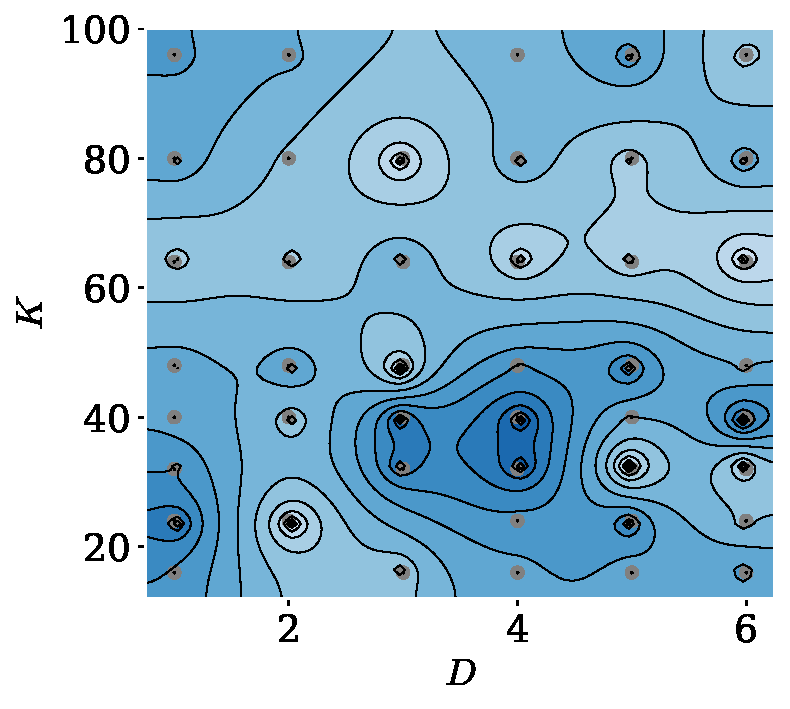
\includegraphics[width=\FW,height=\FH]{Figures/contour_D_vs_K-TDHA.pdf}}
\subfloat[$D'$ vs. $K$]{%
  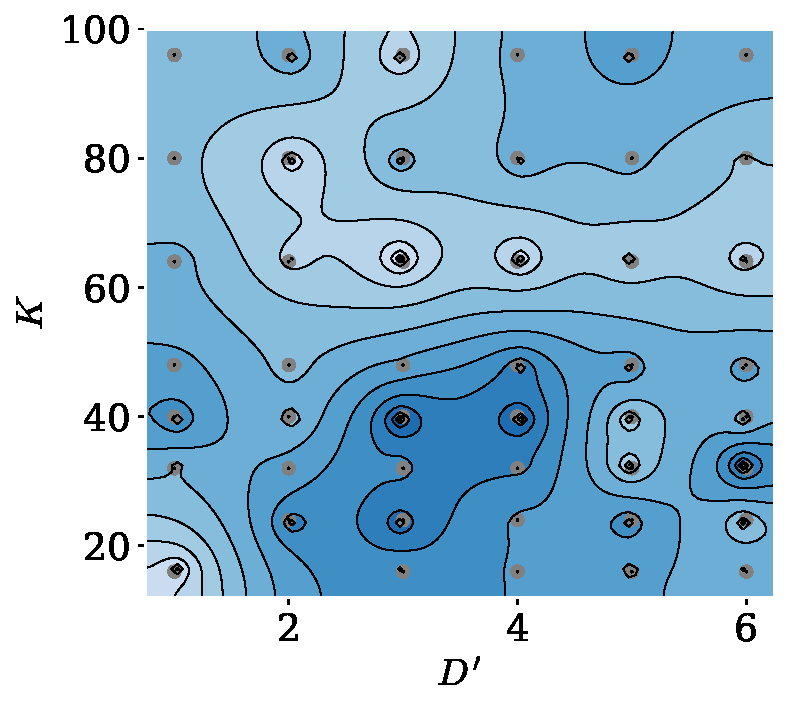
\includegraphics[width=\FW,height=\FH]{Figures/contour_Dprime_vs_K-TDHA.pdf}} 
\subfloat[$D$vs. $\mu$]{%
  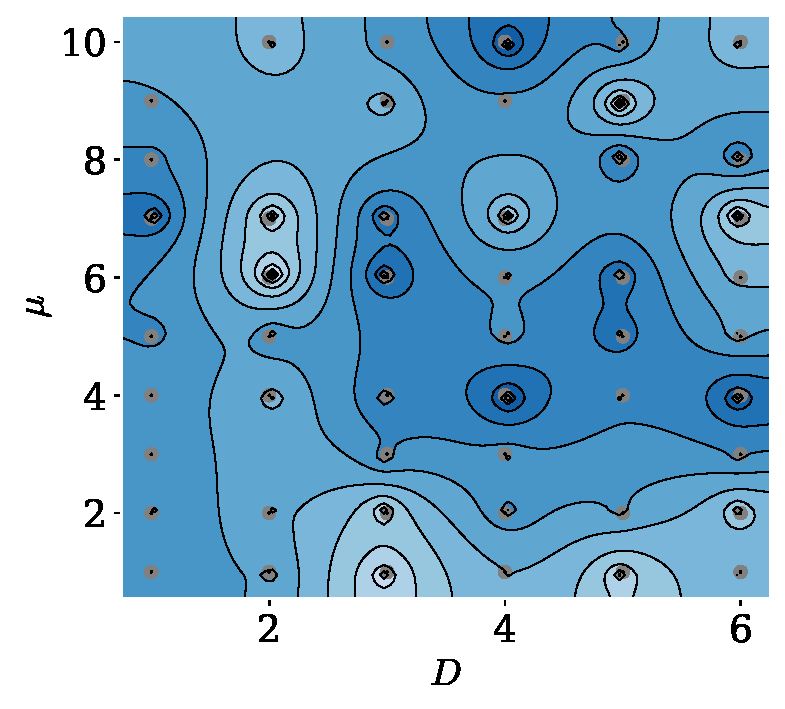
\includegraphics[width=\FW,height=\FH]{Figures/contour_D_vs_mu-TDHA.pdf}} \\[0.6em]

% --------- FILA 2 ----------
\subfloat[$D'$ vs.$\mu$]{%
  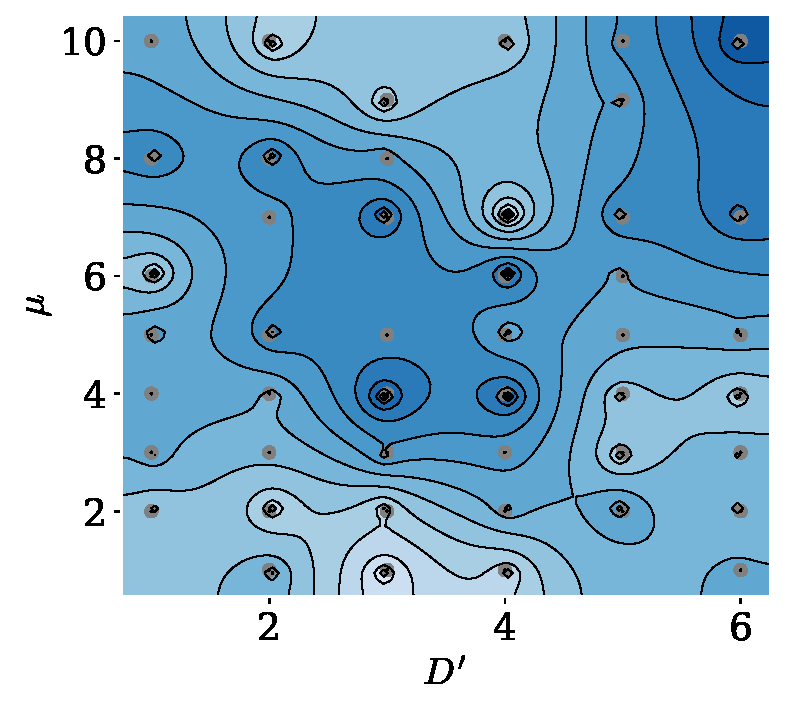
\includegraphics[width=\FW,height=\FH]{Figures/contour_Dprime_vs_mu-TDHA.pdf}} 
\subfloat[$\tau$vs. $\mu$]{%
  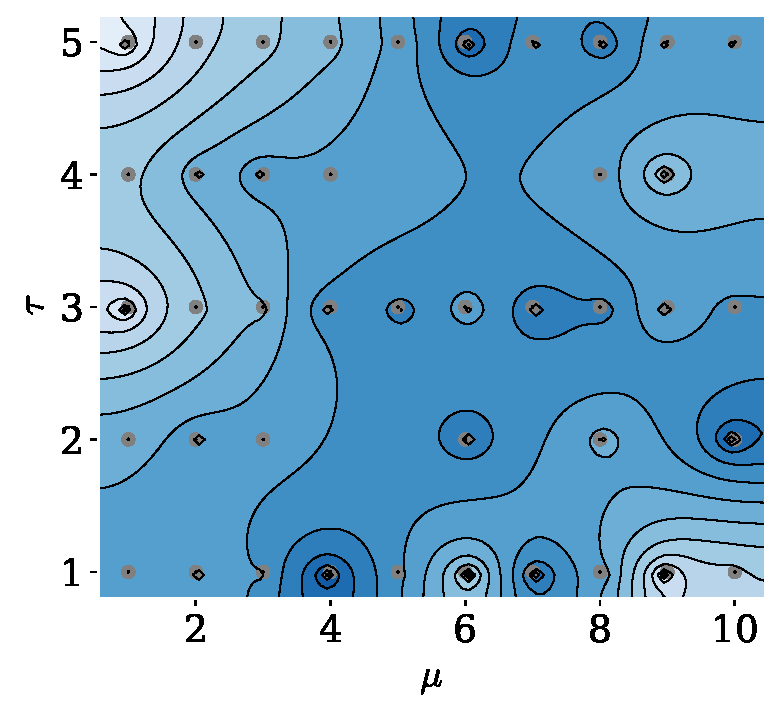
\includegraphics[width=\FW,height=\FH]{Figures/contour_mu_vs_tau-TDHA.pdf}} 
\subfloat[$D'$ vs. $D$]{%
  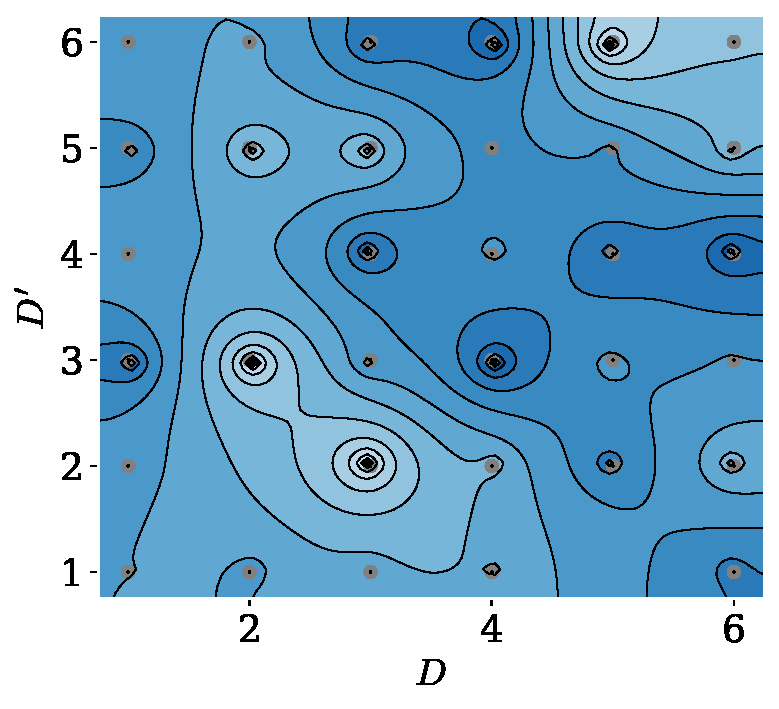
\includegraphics[width=\FW,height=\FH]{Figures/contour_D_vs_Dprime-TDHA.pdf}} \\[0.8em]

% ================= COLORBAR HORIZONTAL (COMPARTIDO) =================
\begin{tikzpicture}
\begin{axis}[
  hide axis,
  scale only axis,
  width=\linewidth,
  height=0pt,
  colormap name=optunablues,
  colorbar horizontal,
  point meta min=57.6,
  point meta max=70.4,
  colorbar style={
    width=\linewidth,
    height=3mm,
    xtick={57.6, 59.2, 60.8, 62.4, 64.0, 65.6, 67.2, 68.8, 70.4},
    xticklabel style={font=\scriptsize},
    xlabel={val accuracy (\%)},
    xlabel style={font=\scriptsize, yshift=2pt},
    scaled ticks=false,
    /pgf/number format/fixed,
    /pgf/number format/precision=1,
  },
]
\addplot [draw=none] coordinates {(0,0)};
\end{axis}
\end{tikzpicture}

\end{minipage}%
}

\caption{{Contour plots of validation accuracy (\%) for \gls{tektenet} as a function of selected hyperparameter pairs under SGKF-CV on the \gls{adhd}/control children dataset. The shared color scale enables direct comparison across hyperparameter interactions within the group-based validation setting.}}
\label{fig:global_freq_tdha}
\end{figure}
%----------------------------------------------------

{To complement the SGKF-CV contour analysis, a global hyperparameter-importance analysis was conducted to quantify the relative contribution of each \gls{tektenet} hyperparameter to validation accuracy on the \gls{adhd}/control children dataset. As shown in Fig.~\ref{fig:TDHA_TE}, this analysis summarizes the influence of the temporal kernel size $K$, the stride $\tau$, the embedding orders $D$ and $D'$, and the interaction delay $\mu$ across the explored hyperparameter configurations, following a functional analysis of variance-based importance estimation strategy~\cite{hutter2014efficient}.}

{The results show that the temporal kernel size $K$ is the most influential hyperparameter, with an importance score of $0.40$, followed by the stride $\tau$ with an importance score of $0.26$. Together, these two parameters account for the largest proportion of the global importance, suggesting that \gls{tektenet} performance on the \gls{adhd}/control children dataset is mainly driven by temporal filtering and stride-related dynamics. This result indicates that, under SGKF-CV, the model depends strongly on how local temporal information is extracted and organized before estimating nonlinear directed interactions.}

{In contrast, the embedding orders $D$ and $D'$ show lower and similar importance scores of $0.12$ and $0.11$, respectively, while the interaction delay $\mu$ also exhibits an importance score of $0.11$. This suggests that state-space reconstruction and delayed directed-dependency modeling still contribute to the validation accuracy, but their influence is secondary compared with the temporal kernel and stride parameters. Overall, these findings indicate that, in the \gls{adhd}/control children dataset, \gls{tektenet} is primarily governed by temporal filtering and compact stride-based temporal encoding, whereas the remaining Takens-based parameters provide complementary adjustments to the effective-connectivity representation~\cite{takens1981detecting,schreiber2000measuring}.}

%------------------------------------------------
\begin{figure}[H]
    \centering
    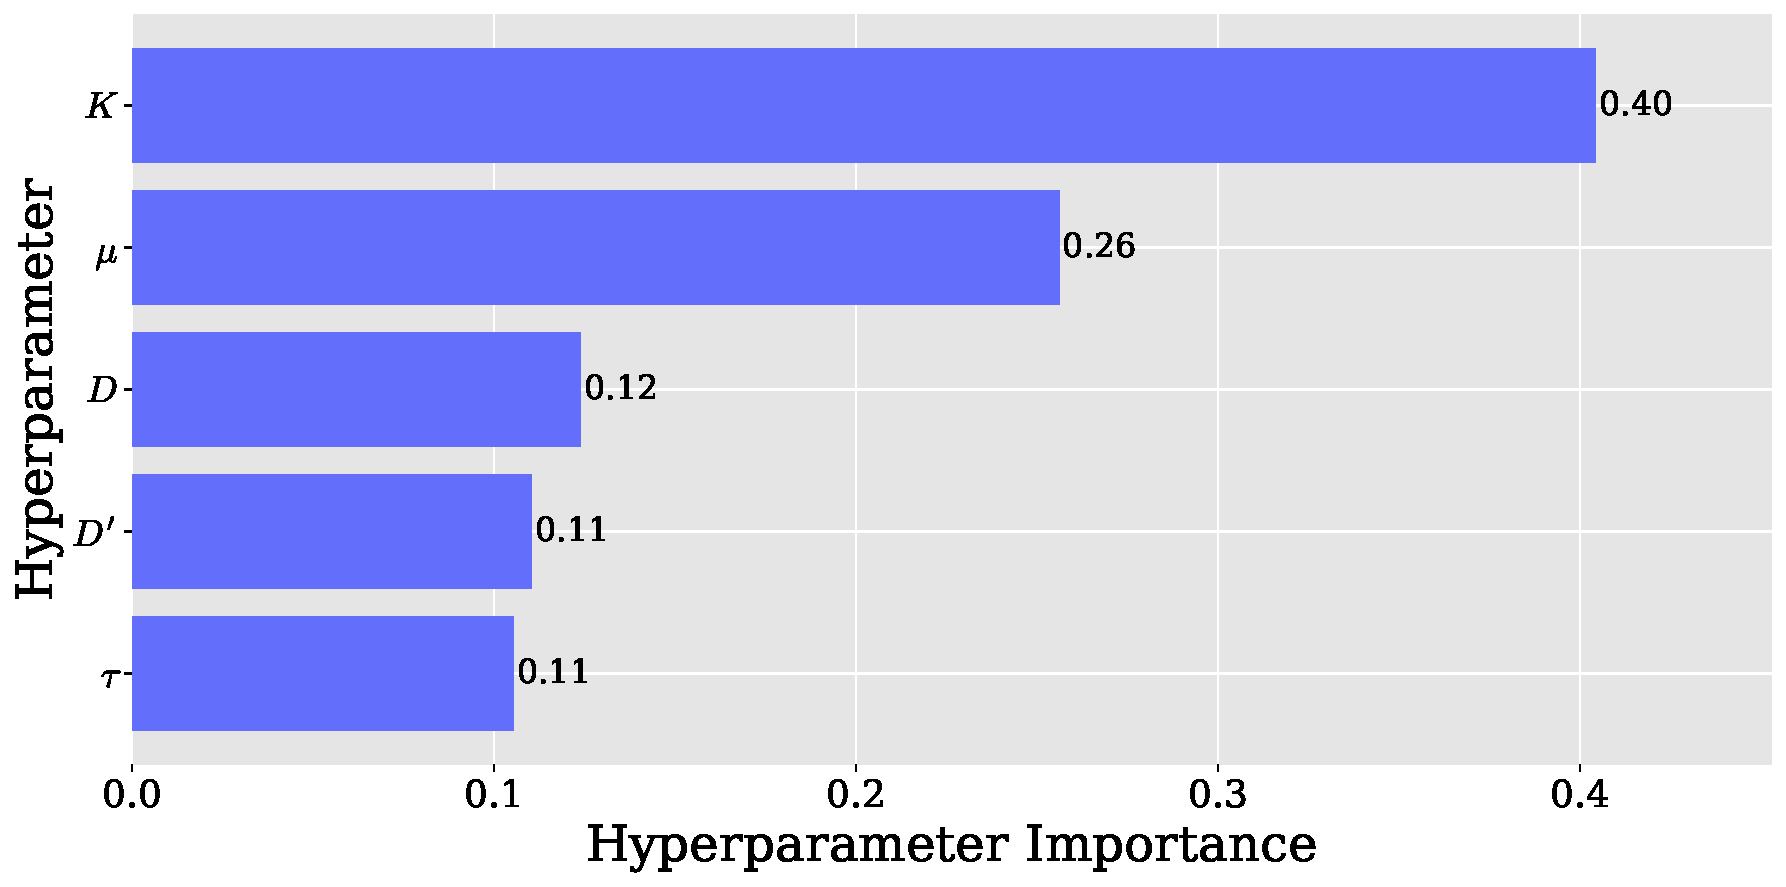
\includegraphics[width=0.8\linewidth]{Figures/optuna_fanova_param_importances_tekte-tdha.pdf}
    \caption{{Global hyperparameter importance analysis for \gls{tektenet} on the \gls{adhd}/control children dataset. Importance scores quantify the relative contribution of the temporal kernel size $K$, stride $\tau$, embedding orders $D$ and $D'$, and interaction delay $\mu$ to validation accuracy under the SGKF-CV protocol.}}
    \label{fig:TDHA_TE}
\end{figure}
%----------------------------------------------------


\subsection{Summary}
\label{sec:Conclu2}

In this chapter, we propose \gls{tektenet}, an end-to-end deep learning model integrating directed \gls{eeg} functional connectivity for \gls{eeg} discrimination. \gls{tektenet} develops an information-theoretic kernelization of \gls{te} within a channel-wise convolutional architecture, enabling the joint modeling of nonlinear delayed and directional neural dependencies. The proposed approach combines five key components. Firstly, a channel-wise convolutional block specializes spectral filters to keep discriminative frequency components. Secondly, a kernelized \gls{te} captures time-delayed signal interactions while preserving causal structure. Third, a Bayesian optimization strategy tunes the architectural hyperparameters to maximize decoding accuracy and to support model interpretability. Fourth, a quadratic kernel formulation enhances robustness to low signal-to-noise ratios, a key characteristic of real-world \gls{eeg} data. Finally, unlike conventional feature engineering or other hybrid approaches, \gls{tektenet} operates in a fully differentiable and end-to-end fashion, without requiring handcrafted features, explicit causality priors, or manual preprocessing steps.

Experimental results across both semi-synthetic causal benchmarks and a real MI-\gls{eeg} dataset demonstrated that \gls{tektenet} accurately recovered the intended causal structures and achieved competitive decoding performance. On semi-synthetic \gls{eeg} data, the model successfully inferred predefined directed interactions, achieving an average validation accuracy above $97\%$. The resulting \gls{te} matrices reproduced the imposed topologies even under Gaussian noise, confirming the framework's ability to identify true directed interactions. The noise analysis revealed that the quadratic kernel variant degrades more slowly as noise levels increase, validating its robustness under varying SNR.

The temporal, spatial, and spectral analyses provided critical insights into both decoding dynamics and underlying neurophysiological processes. Sliding-window experiments confirmed that the 2-4 s post-cue interval consistently yielded the highest decoding performance, aligning with known sensorimotor activation phases during MI. Connectivity visualizations demonstrated clear distinctions between high, medium, and low performing: high-performing subjects exhibited contralaterally organized, sensorimotor-coherent networks, whereas low-performing users showed diffuse, vertically distributed connections lacking lateralization. Spectral analysis of the learned filters further revealed that filters for high-performing subjects preserved power in the $\beta$ ($\approx$20 Hz) and $\gamma$ ($\approx$40 Hz) bands, associated with motor coordination and cognitive engagement, respectively. Conversely, widespread attenuation in low performing reflected diminished task-related activity. These findings provide a direct neurophysiological rationale for the observed decoding variability, 
validates the extraction of neurophysiologically meaningful patterns, and demonstrates the model's interpretability at the network level. 

From an implementation standpoint, \gls{tektenet} maintains a modular and interpretable structure that allows seamless integration into existing BCI pipelines. Its information-theoretic regularization improves robustness to noise, while the kernelized architecture ensures flexibility across subjects and recording conditions. Moreover, the model’s differentiable formulation enables direct gradient-based optimization, fostering explainability and traceability—two features often absent in black-box \gls{eeg} decoders. Nevertheless, estimating pairwise \gls{te} across channels using kernel matrices introduces a computational cost that depends on the number of channels and the lag configuration. Such a cost grows faster for \gls{tektenet} than for standard CNNs. In practice, channel selection strategies may reduce this overhead without degrading performance, thereby facilitating real-time deployment or operation in resource-constrained settings~\cite{Maksimenko}.

In the \gls{adhd}/control classification scenario, the proposed connectivity-based framework exhibited more limited performance compared to the motor imagery experiments. This behavior can be attributed to the increased heterogeneity and complexity of \gls{eeg} patterns associated with \gls{adhd}, which are strongly influenced by developmental variability, attentional fluctuations, and residual nonstationarity, even after extensive preprocessing. Although the kernel-based transfer entropy representations combined with Takens state-space reconstruction enabled the modeling of directed and nonlinear interactions related to altered brain information flow, the obtained results suggest that the current model configuration does not fully exploit the richness of these connectivity representations. In particular, the absence of an extensive hyperparameter tuning process, together with the use of fixed architectural and embedding configurations, may have constrained the discriminative capacity of the model. These findings indicate that further performance improvements could be achieved through more expressive representation learning strategies, including attention-enhanced connectivity models, adaptive hyperparameter optimization, and task-specific architectural refinements. Consequently, the \gls{adhd} results should not be interpreted as a limitation of the connectivity-based approach itself, but rather as evidence of the need for more powerful and adaptive models to address the high variability and complexity inherent to \gls{eeg} data in neurodevelopmental contexts.

